\documentclass{mimosis}

\usepackage{metalogo}

%%%%%%%%%%%%%%%%%%%%%%%%%%%%%%%%%%%%%%%%%%%%%%%%%%%%%%%%%%%%%%%%%%%%%%%%
% Some of my favourite personal adjustments
%%%%%%%%%%%%%%%%%%%%%%%%%%%%%%%%%%%%%%%%%%%%%%%%%%%%%%%%%%%%%%%%%%%%%%%%
%
% These are the adjustments that I consider necessary for typesetting
% a nice thesis. However, they are *not* included in the template, as
% I do not want to force you to use them.

% This ensures that I am able to typeset bold font in table while still aligning the numbers
% correctly.
\usepackage{etoolbox}

\usepackage[binary-units=true]{siunitx}
\DeclareSIUnit\px{px}

\sisetup{%
  detect-all           = true,
  detect-family        = true,
  detect-mode          = true,
  detect-shape         = true,
  detect-weight        = true,
  detect-inline-weight = math,
}

%%%%%%%%%%%%%%%%%%%%%%%%%%%%%%%%%%%%%%%%%%%%%%%%%%%%%%%%%%%%%%%%%%%%%%%%
% Hyperlinks & bookmarks
%%%%%%%%%%%%%%%%%%%%%%%%%%%%%%%%%%%%%%%%%%%%%%%%%%%%%%%%%%%%%%%%%%%%%%%%

\usepackage[%
  colorlinks = true,
  citecolor  = Blue,
  linkcolor  = Blue,
  urlcolor   = Blue,
  ]{hyperref}

\usepackage{bookmark}
\usepackage{braket}
\usepackage[utf8]{inputenc}
\DeclareUnicodeCharacter{2217}{*}

%%%%%%%%%%%%%%%%%%%%%%%%%%%%%%%%%%%%%%%%%%%%%%%%%%%%%%%%%%%%%%%%%%%%%%%%
% Bibliography
%%%%%%%%%%%%%%%%%%%%%%%%%%%%%%%%%%%%%%%%%%%%%%%%%%%%%%%%%%%%%%%%%%%%%%%%
%
% I like the bibliography to be extremely plain, showing only a numeric
% identifier and citing everything in simple brackets. The first names,
% if present, will be initialized. DOIs and URLs will be preserved.

\usepackage[%
  autocite     = plain,
  backend      = bibtex,
  doi          = true,
  url          = true,
  giveninits   = true,
  hyperref     = true,
  maxbibnames  = 3,
  maxcitenames = 3,
  sortcites    = true,
  style        = numeric,
  ]{biblatex}

%%%%%%%%%%%%%%%%%%%%%%%%%%%%%%%%%%%%%%%%%%%%%%%%%%%%%%%%%%%%%%%%%%%%%%%%
% Some adjustments to make the bibliography more clean
%%%%%%%%%%%%%%%%%%%%%%%%%%%%%%%%%%%%%%%%%%%%%%%%%%%%%%%%%%%%%%%%%%%%%%%%
%
% The subsequent commands do the following:
%  - Removing the month field from the bibliography
%  - Fixing the Oxford commma
%  - Suppress the "in" for journal articles
%  - Remove the parentheses of the year in an article
%  - Delimit volume and issue of an article by a colon ":" instead of
%    a dot ""
%  - Use commas to separate the location of publishers from their name
%  - Remove the abbreviation for technical reports
%  - Display the label of bibliographic entries without brackets in the
%    bibliography
%  - Ensure that DOIs are followed by a non-breakable space
%  - Use hair spaces between initials of authors
%  - Make the font size of citations smaller
%  - Fixing ordinal numbers (1st, 2nd, 3rd, and so) on by using
%    superscripts

% Remove the month field from the bibliography. It does not serve a good
% purpose, I guess. And often, it cannot be used because the journals
% have some crazy issue policies.
\AtEveryBibitem{\clearfield{month}}
\AtEveryCitekey{\clearfield{month}}

% Fixing the Oxford comma. Not sure whether this is the proper solution.
% More information is available under [1] and [2].
%
% [1] http://tex.stackexchange.com/questions/97712/biblatex-apa-style-is-missing-a-comma-in-the-references-why
% [2] http://tex.stackexchange.com/questions/44048/use-et-al-in-biblatex-custom-style
%
\AtBeginBibliography{%
  \renewcommand*{\finalnamedelim}{%
    \ifthenelse{\value{listcount} > 2}{%
      \addcomma
      \addspace
      \bibstring{and}%
    }{%
      \addspace
      \bibstring{and}%
    }
  }
}

% Suppress "in" for journal articles. This is unnecessary in my opinion
% because the journal title is typeset in italics anyway.
\renewbibmacro{in:}{%
  \ifentrytype{article}
  {%
  }%
  % else
  {%
    \printtext{\bibstring{in}\intitlepunct}%
  }%
}

% Remove the parentheses for the year in an article. This removes a lot
% of undesired parentheses in the bibliography, thereby improving the
% readability. Moreover, it makes the look of the bibliography more
% consistent.
\renewbibmacro*{issue+date}{%
  \setunit{\addcomma\space}
    \iffieldundef{issue}
      {\usebibmacro{date}}
      {\printfield{issue}%
       \setunit*{\addspace}%
       \usebibmacro{date}}%
  \newunit}

% Delimit the volume and the number of an article by a colon instead of
% by a dot, which I consider to be more readable.
\renewbibmacro*{volume+number+eid}{%
  \printfield{volume}%
  \setunit*{\addcolon}%
  \printfield{number}%
  \setunit{\addcomma\space}%
  \printfield{eid}%
}

% Do not use a colon for the publisher location. Instead, connect
% publisher, location, and date via commas.
\renewbibmacro*{publisher+location+date}{%
  \printlist{publisher}%
  \setunit*{\addcomma\space}%
  \printlist{location}%
  \setunit*{\addcomma\space}%
  \usebibmacro{date}%
  \newunit%
}

% Ditto for other entry types.
\renewbibmacro*{organization+location+date}{%
  \printlist{location}%
  \setunit*{\addcomma\space}%
  \printlist{organization}%
  \setunit*{\addcomma\space}%
  \usebibmacro{date}%
  \newunit%
}

% Do not abbreviate "technical report".
\DefineBibliographyStrings{english}{%
  techreport = {technical report},
}

% Display the label of a bibliographic entry in bare style, without any
% brackets. I like this more than the default.
%
% Note that this is *really* the proper and official way of doing this.
\DeclareFieldFormat{labelnumberwidth}{#1\adddot}

% Ensure that DOIs are followed by a non-breakable space.
\DeclareFieldFormat{doi}{%
  \mkbibacro{DOI}\addcolon\addnbspace
    \ifhyperref
      {\href{http://dx.doi.org/#1}{\nolinkurl{#1}}}
      %
      {\nolinkurl{#1}}
}

% Use proper hair spaces between initials as suggested by Bringhurst and
% others.
\renewcommand*\bibinitdelim {\addnbthinspace}
\renewcommand*\bibnamedelima{\addnbthinspace}
\renewcommand*\bibnamedelimb{\addnbthinspace}
\renewcommand*\bibnamedelimi{\addnbthinspace}

% Make the font size of citations smaller. Depending on your selected
% font, you might not need this.
\renewcommand*{\citesetup}{%
  \biburlsetup
  \small
}

\DeclareLanguageMapping{british}{bibliography-correct-ordinals}
\DeclareLanguageMapping{english}{bibliography-correct-ordinals}

\bibliography{library.bib}

%%%%%%%%%%%%%%%%%%%%%%%%%%%%%%%%%%%%%%%%%%%%%%%%%%%%%%%%%%%%%%%%%%%%%%%%
% Fonts
%%%%%%%%%%%%%%%%%%%%%%%%%%%%%%%%%%%%%%%%%%%%%%%%%%%%%%%%%%%%%%%%%%%%%%%%

\ifxetexorluatex
  \setmainfont{Minion Pro}
\else
  \usepackage[lf]{ebgaramond}
  \usepackage[oldstyle,scale=0.7]{sourcecodepro}
  \singlespacing
\fi


\makeindex
\makeglossaries

%%%%%%%%%%%%%%%%%%%%%%%%%%%%%%%%%%%%%%%%%%%%%%%%%%%%%%%%%%%%%%%%%%%%%%%%
% Incipit
%%%%%%%%%%%%%%%%%%%%%%%%%%%%%%%%%%%%%%%%%%%%%%%%%%%%%%%%%%%%%%%%%%%%%%%%

\bibliography{library.bib}
\begin{document}

\frontmatter
  % !TEX root = ./upgradeReport.tex
\begin{titlepage}
%\vspace*{-1.5in}\hspace*{-9.7in}\includegraphics[width=2\paperwidth]{uclbannerblack}
\vspace*{-1in}\hspace*{-1.5in}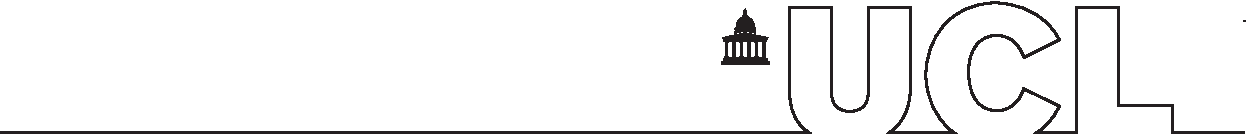
\includegraphics[width=1.02\paperwidth]{UCLlogo}
\newcommand{\HRule}{\rule{\linewidth}{0.5mm}} % Defines a new command for the
% horizontal lines, change thickness here
\null\vfil
\center % Center everything on the page
 \textsc{\LARGE University College London}
 % Name of your
% university/college
\\[1cm]
\textsc{\Large UCL PhD Upgrade Report}\\[0.5cm] % Major
% heading such as course name \textsc{\large Literature Review}\\[0.5cm] % Minor heading such as course title


\HRule \\[0.2cm]
{\LARGE \bfseries Towards an interface between an optically addressed, mechanically mobile probe qubit and data qubits in silicon}\\[-0.2cm]
% Title of your document
\HRule \\[1.2cm]

\begin{minipage}[t]{0.4\textwidth}
\begin{flushleft} \large
\emph{Author:}\\
David F. \textsc{Wise}% Your name
\end{flushleft}
\end{minipage}
\begin{minipage}[t]{0.4\textwidth}
\begin{flushright} \large
\emph{Supervisor:} \\
Prof. John \textsc{Morton} \\% Supervisor's Name
\end{flushright}
\end{minipage}\\[2cm]

{\large \today}\\% Date, change the \today to a set date if you want to
% be precise

%\includegraphics{Logo}\\[1cm] % Include a department/university logo - this
% will require the graphicx package

\null\vfil % Fill the rest of the page with whitespace
\end{titlepage}

  \begin{center}
  \textsc{Abstract}
\end{center}
%
\noindent
%
Scientific documents often use \LaTeX{} for typesetting. While numerous
packages and templates exist, it makes sense to create a new one. Just
because.


  \tableofcontents

\mainmatter
  % !TEX root = Thesis.tex
% \listoffigures
% !TEX root = ../Thesis.tex

\chapter{Introduction}
% \begin{center}
% \begin{minipage}{0.5\textwidth}
% \begin{small}
% \emph{At midnight all the agents and superhuman crew come out and round up everyone who knows more than they do}
% \end{small}
% \end{minipage}
% \vspace{0.5cm}
% \end{center}
Quantum computing has been an active field of research since the concept was first suggested by Richard Feynman in the early 1980s \cite{Feynman1982}.
Originally proposed as an efficient method for simulating chemical processes (something that traditional computers find extremely taxing) the discovery of several algorithms offering significant speed increases over classical computers has further fuelled research \cite{Shor1994,Shor1997}.
Strong initial scepticism abounded regarding the potential for quantum computers to exist in the real world, primarily due to the concerns that error correction with such a complex device would be impossible\cite{Preskill1997}.
This pessimism gave way with the identification of an error threshold for quantum computation.
Given an error rate below a critical threshold it was possible to perform an arbitrarily long computation with negligible possibility of significant error \cite{Shor1996,Aharonov1997}.
Following these discoveries serious attention has been given to the development of error correcting codes that might be implemented to allow a physical quantum computer to be \emph{fault tolerant}.
\\
Gottesman identified the class of error correcting codes known as \emph{stabilizer codes}, defined by the group of logical operators that leave the code unchanged \cite{Gottesman1997a}.
This class of quantum error correcting codes has become the dominant form in theoretical research.
Of these \emph{the surface code}, developed by Bravyi and Kitaev \cite{Bravyi1998}, has become pre-eminent in experimental efforts.
Although other quantum error correcting codes (such as colour codes \cite{Vasmer2018}) exist, the surface code has become the focus for experimental implementations. This is due mainly to the relatively high error threshold, $\sim0.5\%$, and the simple architecture of a planar grid of qubits.
\\
In recent years there has been rapid progress in the development of physical qubits.
Groups in both the academic and private sectors have shown small numbers of qubits functioning with error rates above the fault tolerant threshold \cite{Barends2015,Reagor2017}.
The successful recent approaches have tended to focus on superconducting circuits to produce their qubits.
Whilst these have proved excellent for the small numbers of qubits currently in use, it is likely that they will present significant additional challenges when scaling to numbers sufficient for useful, fault-tolerant quantum computation.
With the numbers required likely to be close to $100 \times 10^6$ and the current size of these qubits close to 1~mm$^2$, it will likely be impossible to use these qubits in their current form in a fault-tolerant quantum computer.
\\
Although there are many alternative systems that could provide a qubit, this paper will focus on the use of the spins of nuclei and electrons bound to donors in semiconductors, particularly silicon.
A seminal paper by Kane \cite{Kane1998} stimulated much of the research interest in this field.
He proposed using the spin of phosphorus nuclei in silicon as qubits with the ability to mediate interactions between neighbouring donor nuclei using the interaction between the electrons bound to each.
These types of qubit are attractive due to their exceptionally long coherence times: the time that the qubit reliably stores quantum information for. 
A long coherence time relative to qubit gate times is essential, as this determines the error rate of the qubits.
Coherence times as long as several seconds have been reported for donor spin qubits in silicon, whilst gate times can be as short as several nanoseconds \cite{Wolfowicz2013}. 
Despite these advantages, development of these types of qubits for quantum computers has lagged behind the superconducting and ion trap versions \cite{Ballance2015}. 
This is due to the difficulty of isolating and addressing single donors in a silicon lattice. 
Kane's proposal required sub nano-metre precision in qubit placement to facilitate inter-qubit interactions. 
Even if this precision were achieved there remains the issue of how the requisite control circuitry could be integrated into such a dense design.
This has lead to the development of more modern proposals to both overcome these difficulties and also to implement surface code based error correction.
\\
\\
One such proposal is from O'Gormann et al \cite{OGorman2014}. 
This proposal takes a similar approach to Kane, with qubits being donor spins in a silicon lattice. 
Where it differs significantly is in its use of two lattices of qubits. 
One of these is for the storage of data, whilst the other performs measurements on these data qubits. 
This measurement stage is placed above the data stage and held close, within 40~nm, and moved in a repeating cycle over the data qubits.
This allows each measurement qubit to perform $\hat{X}$ or $\hat{Z}$ measurement on groups of four data qubits, the stabilizer measurements that make up the fundamental units of surface code.
This architecture allows for data qubits to be placed much farther apart - since no direct interaction between them is required.
Several key research questions remain:
\begin{enumerate}
	\item{What donor species should be used for both types of qubit?}
	\item{How are the measurement qubits to be read out?}
	\item{How are the qubits to be controlled?}
\end{enumerate}
Whilst donors in silicon make excellent choices for the data qubits due to the properties stated above, a different qubit species is required for the measurement qubits to avoid an unwanted exchange interaction between the two lattices.
Optical qubit readout is suggested in the proposal by O'Gormann et al and is a well studied means of reading the state of spin qubits, particularly in nitrogen-vacancy (NV) centres in diamond \cite{Liu2017}.
A concern with optical readout is the impact that illumination can have on the coherence times of donors in silicon. 
Silicon has a band gap energy equivalent to approximately 1058~nm or photon energy of 1.17~eV. 
Illumination at shorter wavelengths than this will create free electrons in the silicon conduction band.
These can scatter off the electrons bound to donors, causing them to relax and shortening the $T_1$ time of the qubits as a whole \cite{Ross2017a}.
NV centres are read out at between 500~nm and 600~nm, illumination that would reduce data qubit coherence times and increase the qubit error rate. 
Alternative optically addressed spin qubits at higher wavelengths exist, such as the di-vacancy centre in silicon carbide \cite{Christle2014}, but a vital question is what wavelengths can be used for read-out without compromising data qubit coherence times.
This report addresses this question by examining the effect of various laser wavelengths close to the silicon band gap on the coherence times of electrons bound to phosphorus donors in silicon.
\\
Another key question presented by the O'Gormann proposal is what data qubits to select and how to control them.
The frequencies traditionally used for electron spin resonance are between 8~GHz and 10~GHz. 
Electromagnetic radiation at these frequencies require large coaxial cables and cavities for transmission. 
This makes it almost impossible to individually address qubits using microwaves. 
Instead the solution proposed by Kane is to use global microwave pulses, addressing all qubits at once.
To selectively control qubits the DC Stark shift can be employed - DC electric fields can be used to shift the electron spin transition frequency meaning that a global microwave field will not effect them. 
Unlike RF radiation, DC signals are easily multiplexed and the commercial electronics industry has achieved fabrication precision well within that required by the O'Gormann proposal.
In addition to the potential control benefits provided by the Stark shift, it can bring problems. 
Inhomogeneous electric fields near spin qubits would alter the energy of their transition, potentially leading to decoherence.
It is also beneficial, therefore, to identify systems that only experience a small Stark shift, as this would render them much more resistant to electric field noise and make them potentially ideal data qubits.
One such system is explored in this report, the unpaired electron bound to a selenium$+$ donor in silicon.
One further area of interest is the potential integration of a quantum memory into the data qubit lattice.
The spin-$\frac{1}{2}$ $^{29}$Si nuclei are normally viewed as a nuisance due to their reducing the coherence times of electrons bound to donors in silicon.
They have, however, been shown as a potential quantum register for these donor qubits, due to their long coherence times.
The Stark shift offers a potential means to control the interaction between data qubits and a $^{29}$Si based quantum memory in natural silicon.
As such a final focus of this paper will be an attempt to measure the Stark shift of the interaction between the $^{29}$Si nuclei and the electrons bound to phosphorus donors in silicon.






% !TEX root = ../Thesis.tex

\chapter{Spin Defects}

\section{Electron Spin Resonance}
\subsection{Spin States}

Paramagnetic defects in crystals are one of the major experimental areas under investigation as potential qubit platforms. This thesis will focus on the paramagnetic defects found in two semiconductor crystals: silicon and diamond. In silicon, neutrally charged group V donors offer a system analogous to a Hydrogen atom: a single unpaired electron bound to a nucleus with a net positive charge. Both electron and nucleus in this system have the property of intrinsic angular momentum or \emph{spin}, $\mathbf{S}$, a vector property of the system with components $S_x, S_y, S_z$. The projection of the particle's spin along any given axis is one of a series of discrete values dependent on the total spin of the system and spaced by integer values of $\hbar$. Typically and from here $\hbar$ is treated as being equal to 1 for ease of calculations. The electron is a spin-$\frac{1}{2}$ particle and can take only the values (or eignestates) $-\frac{1}{2},\frac{1}{2}$. A nucleus, however, may have a variety of different spin values. Phosphorus donors in silicon have a spin-$\frac{1}{2}$ nucleus whilst Bismuth donors have a spin-$\frac{9}{2}$ nucleus. As the $S_{x,y,z}$ operators are non-commuting, the spin can have a defined value in only one cartesian dimension, usually defined as $S_z$. For a free electron, not in the presence of a magnetic field, space is isotropic, meaning any axis can be specified as $S_z$ and the two eigenstates $\pm\frac{1}{2}$ are degenerate in energy.

Associated with the spin of a particle is a magnetic dipole moment, $\mathbf{\mu}$, that determines the degree of interaction between the particle and a magnetic field, known as the Zeeman interaction \cite{10003989896}. For an electron, this moment, $\mu_e$, is equal to $-g\mu_b\mathbf{S}$ where $\mu_b$ = $\frac{e\hbar}{2m_e}$. The energy of this dipole interacting with a magnetic field, $\mathbf{B}$, is then equal to $-g\mu_b\mathbf{S}\cdot\mathbf{B}$. In practice the $S_z$-axis of the spin is defined as being aligned with the magnetic field giving two spin eigenstates. The Hamiltonian governing the electron spin can then be written:

\begin{equation}
H = -g\mu_bB_0S_z
\label{eq:freeelecham}
\end{equation}

Where $B_0$ is the magnitude of the magnetic field $|\mathbf{B}|$. This Hamiltonian then gives two spin eigenstates, designated as $\ket{0}$ and $\ket{1}$ or $\ket{\uparrow}$ and $\ket{\downarrow}$, corresponding to the spin being aligned and anti-aligned with the magnetic field. The energy difference between these states is:

\begin{equation}
\Delta E = g_e\mu_bB,
\label{eq:enSplit}
\end{equation}

This results in an energy splitting as seen in figure \ref{fig:elecSplit} a. Typically, the energy level splittings are referred to by their frequency, according to the equation $E = h\nu$, as this gives the frequency of a microwave pulse resonant with the transition.

In practice, electrons bound to defects in semiconductors are not free, and cannot be described fully by the simple Hamiltonian shown in \ref{eq:freeelecham}. The chief reason for this is that the electron will be bound to a nucleus with its own spin state, $\mathbf{I}$. To account for the nucleus, the Hamiltonian requires the addition of two further terms: one to account for the hyperfine interaction and one to account for the nuclear spin's interaction with the magnetic field. The hyperfine interaction refers to the effect of the magnetic fields from electron and nucleus interacting with each other. This interaction leads to two possible energy states, where electron and nuclear spin are aligned (higher energy) and where they are anti-aligned (lower energy). Due to the small nuclear magneton, $\mu_N$ of the nucleus, the hyperfine interaction is typically a significantly greater energy effect than that of the nuclear Zeeman term, except at very high magnetic fields (>1~T). The full Hamiltonian of the electron-nuclear spin system can be written as follows \cite{landlifquantmech}:

\begin{equation}
  \hat{H} = -g\mu_b\mathbf{B}\cdot\mathbf{S} + g_I\mu_N\mathbf{B}\cdot\mathbf{I} + \hat{A}\mathbf{S}\cdot\mathbf{I}
  \label{eqn:phos-ham}
\end{equation}

The energy level structure of a phosphorus donor in silicon is described by this Hamiltonian. The phosphorus nucleus, like the electron, is a spin-$\frac{1}{2}$ system ($I = 1/2$), meaning that the joint system has a four level  structure shown in figure \ref{fig:elecSplit}b. At low magnetic fields, this has a singlet ($m_s = 0$) - triplet ($m_s = 1$) structure, due to the dominance of the hyperfine splitting term over the Zeeman terms. At these low fields the spin projection in the $B_0$ direction ($S_z$) of the electron and nucleus does not represent a good quantum number - meaning that the projection will \emph{not} remain constant under time evolution, instead it is their total spin that best represents the system state. At high magnetic fields, where the Zeeman term dominates, the degeneracy of the triplet state is lifted and four well defined energy levels emerge. At these high fields the spin states of electron and nucleus are isolated, meaning their $z$-projection is a good quantum number. Most experiments with phosphorus donors in silicon are performed at these high fields.

\begin{figure}
\centering
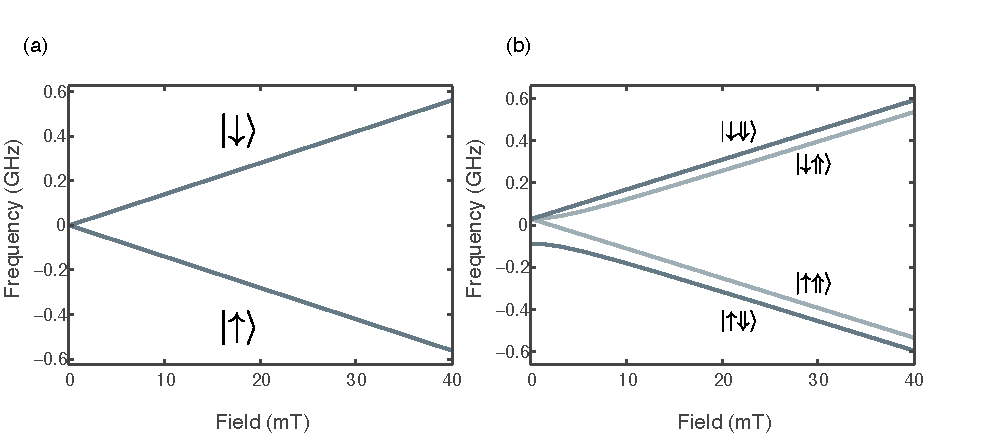
\includegraphics[width = \columnwidth]{Plotting/Figs/all-levels-fig.pdf}
\caption[Energy level splittings for a free electron and an electron bound to a phosphorus donor in silicon]{(a) the energy level splitting of a free electron in a magnetic field, showing how separation in energy increases with magnetic field. (b) the energy level splitting of the spin states of a phosphorus spin system in a magnetic field. $\ket{\uparrow}$ refers to the electron spin state and $\ket{\Uparrow}$ to the nuclear spin state. Note the lower energy state of the anti-aligned nuclear spin state for a given electron spin state, due to the dominance of the hyperfine coupling term over the nuclear Zeeman term in equation~\ref{eqn:phos-ham}.}
\label{fig:elecSplit}
\end{figure}

In addition to causing this level splitting, the magnetic field will also cause the electron spin to precess about the magnetic field at the Larmor frequency, given by:
\begin{equation}
  \omega_0 = \frac{g \mu_B}{\hbar}B_0
\end{equation}

\subsection{The Bloch Sphere}
\label{seq:blochSphere}

The eigenstates of the electron spin in a magnetic field allow the spin to be described as a two level system and represented on the \emph{Bloch Sphere} \cite{Bloch1946,Schweiger}. The Bloch sphere provides a convenient method for representing and visualising quantum states. The two spin states form a basis and are represented by the kets $\ket{0}$ and $\ket{1}$ corresponding to up and down spin or low and high energy levels. These form the North and South poles of the Bloch sphere resepectively. As well as these two spin eigenstates, any linear superposition of them is also a valid state of the system~\cite{Nielsen:2011:QCQ:1972505}:

\begin{equation}
  \ket{\psi} = \alpha\ket{0} + \beta\ket{1}
\end{equation}

If the condition that $\sqrt{|\alpha^2| + |\beta^2|}$ is met than this state is said to be `pure'. All of these pure states of the system are represented by points on the surface of the Bloch sphere. Mixed states, where some classical uncertainty is taken into account in the states representation, fall inside the sphere.

\begin{figure}
  \centering
  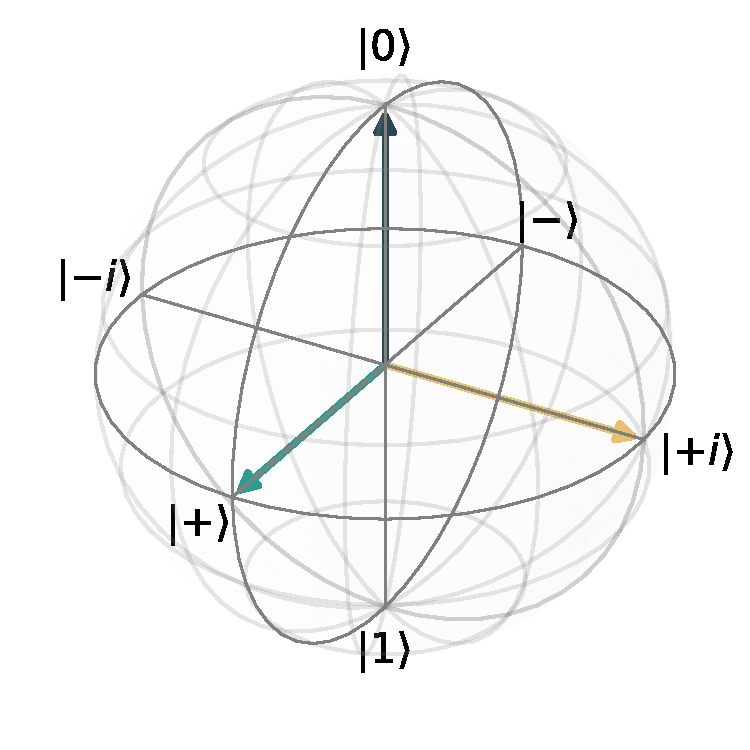
\includegraphics[width=0.5\columnwidth]{/Plotting/Figs/bloch_simple.pdf}
  \caption[The Bloch sphere and Pauli operator eigenstates]{Figure showing the Bloch sphere representation of qubit states. The states shown are the eigenstates of the 3 Pauli spin operators ($S_z \rightarrow [\ket{0}, \ket{1}], S_x \rightarrow [\ket{+}, \ket{-}], S_y \rightarrow [\ket{+i}, \ket{-i}])$, with the states associated with the positive eigenvalue marked by arrows.}
  \label{fig:bloch_simple}
\end{figure}

\subsection{Driving Spin Transitions}


A sufficiently strong static magnetic field, $B_0$, splits the electron energy states and gives the spin eigenstates $\ket{0}$ and $\ket{1}$ but gives no way of driving transitions to other states on the Bloch sphere. To achieve this, a second magnetic field, $B_1$, is typically applied perpendicular to the static field.  The spin will precess around this second magnetic field at the Larmor frequency determined by its field strength~\cite{Schweiger}. A static $B_1$ field can be used as long as the Larmor frequency of this field is significantly faster than that of the $B_0$ field, meaning that precession around $B_0$ can be disregarded whilst the $B_1$ field is applied. In reality, it is not practical to apply such a strong field, so instead a field is applied via an oscillating magnetic field. This will mean that the $B_1$ field will rotate in the $x-y$ plane of the Bloch sphere at $\omega$, the Hamiltonian of this process can then be written:

\begin{equation}
  H = g \mu_B B_0 S_z + g\mu_BB_1 \cos(\omega t)S_x
\end{equation}

For convenience of calculation and understanding, it is typical to perform a transformation on this Hamiltonian into the \emph{rotating frame} by applying the following transformation:
\begin{equation}
  U =
  \begin{pmatrix}
    e^{i \omega t} & 0 \\
    0 & e^{- i \omega t}
  \end{pmatrix}
\end{equation}

This results in the Hamiltonian in the rotating frame being:
\begin{equation}
  \tilde{H} =
  \begin{pmatrix}
    \frac{1}{2}(\omega - \omega_0) & \omega_1 \cos(\omega t) e^{-i \omega t} \\
    \omega_1 \cos(\omega t) e^{i \omega t} & \frac{1}{2}(\omega - \omega_0)
  \end{pmatrix}
\end{equation}

Where $\omega_0$ is the Larmor precession frequency of the $B_0$ field, $\omega_1$ is the precession frequency of the $B_1$ field and $\omega$ is the frequency of oscillation of the $B_1$ field. The counter-rotating terms in the off-diagonal elements of the Hamiltonian can be ignored, as they oscillate quickly relative the the spin (effectively, far off resonance) and so provide only a minor perturbation to its evolution. As such, the final Hamiltonian in the rotating frame can be written:

\begin{equation}
  \tilde{H} =
  \begin{pmatrix}
    \frac{1}{2}(\omega - \omega_0) & \frac{\omega_1}{2} \\
    \frac{\omega_1}{2} & \frac{1}{2}(\omega - \omega_0)
  \end{pmatrix}
\end{equation}

The diagonal elements of this Hamiltonian depend on the detuning between the Larmor precession frequency of the applied $B_0$ field and the frequency of the $B_1$ field and go to 0 when these are on resonance. So the Hamiltonian at resonance is effectively:

\begin{equation}
  \tilde{H} = \frac{\omega_1}{2} \sigma_x
\end{equation}


This allows the precession of the qubit in the static magnetic field to be disregarded, along with the precession of the oscillating $B_1$ field. The application of an on-resonance $B_1$ field will cause a $\ket{0}$ state to precess about the $x$-axis at the Larmor frequency of that field. Off-resonance dynamics are more complex, causing precession about an axis in the Bloch sphere determined by the detuning of the $B_1$ field. As detuning increases, the angle of rotation varies quickly relative to the spin vector, meaning that at large detunings the rotational effect averages out and can be ignored - except in cases where the $B_1$ field is comparable to $B_0$ in magnitude. In most experiments the $|B_1| \ll |B_0|$ requirement holds and the effect of a strongly detuned $B_1$ field can be disregarded. Figure \ref{fig:rabi-dynamics} shows the behaviour of the spin state on the Bloch sphere in the case of both on and off-resonance excitation. The frequency at which the spin rotates in the $B_1$ field when on-resonance is usually termed the \emph{rabi}-frequency and is often designated by $\Omega$. By varying the time the $B_1$ field is applied for, the spin can be rotated to any point on the $z-y$ plane of the Bloch sphere. To perform arbitrary rotations on the Bloch sphere, the phase of the applied $B_1$ field can be varied. This will cause the spin to precess about an axis in the $x-y$ plane, whose angle from the $x$-axis is determined by the phase of the $B_1$ field. By varying this phase and the time the field is applied for it can be used to rotate the qubit to any point on the Bloch sphere.



\begin{figure}
  \centering
  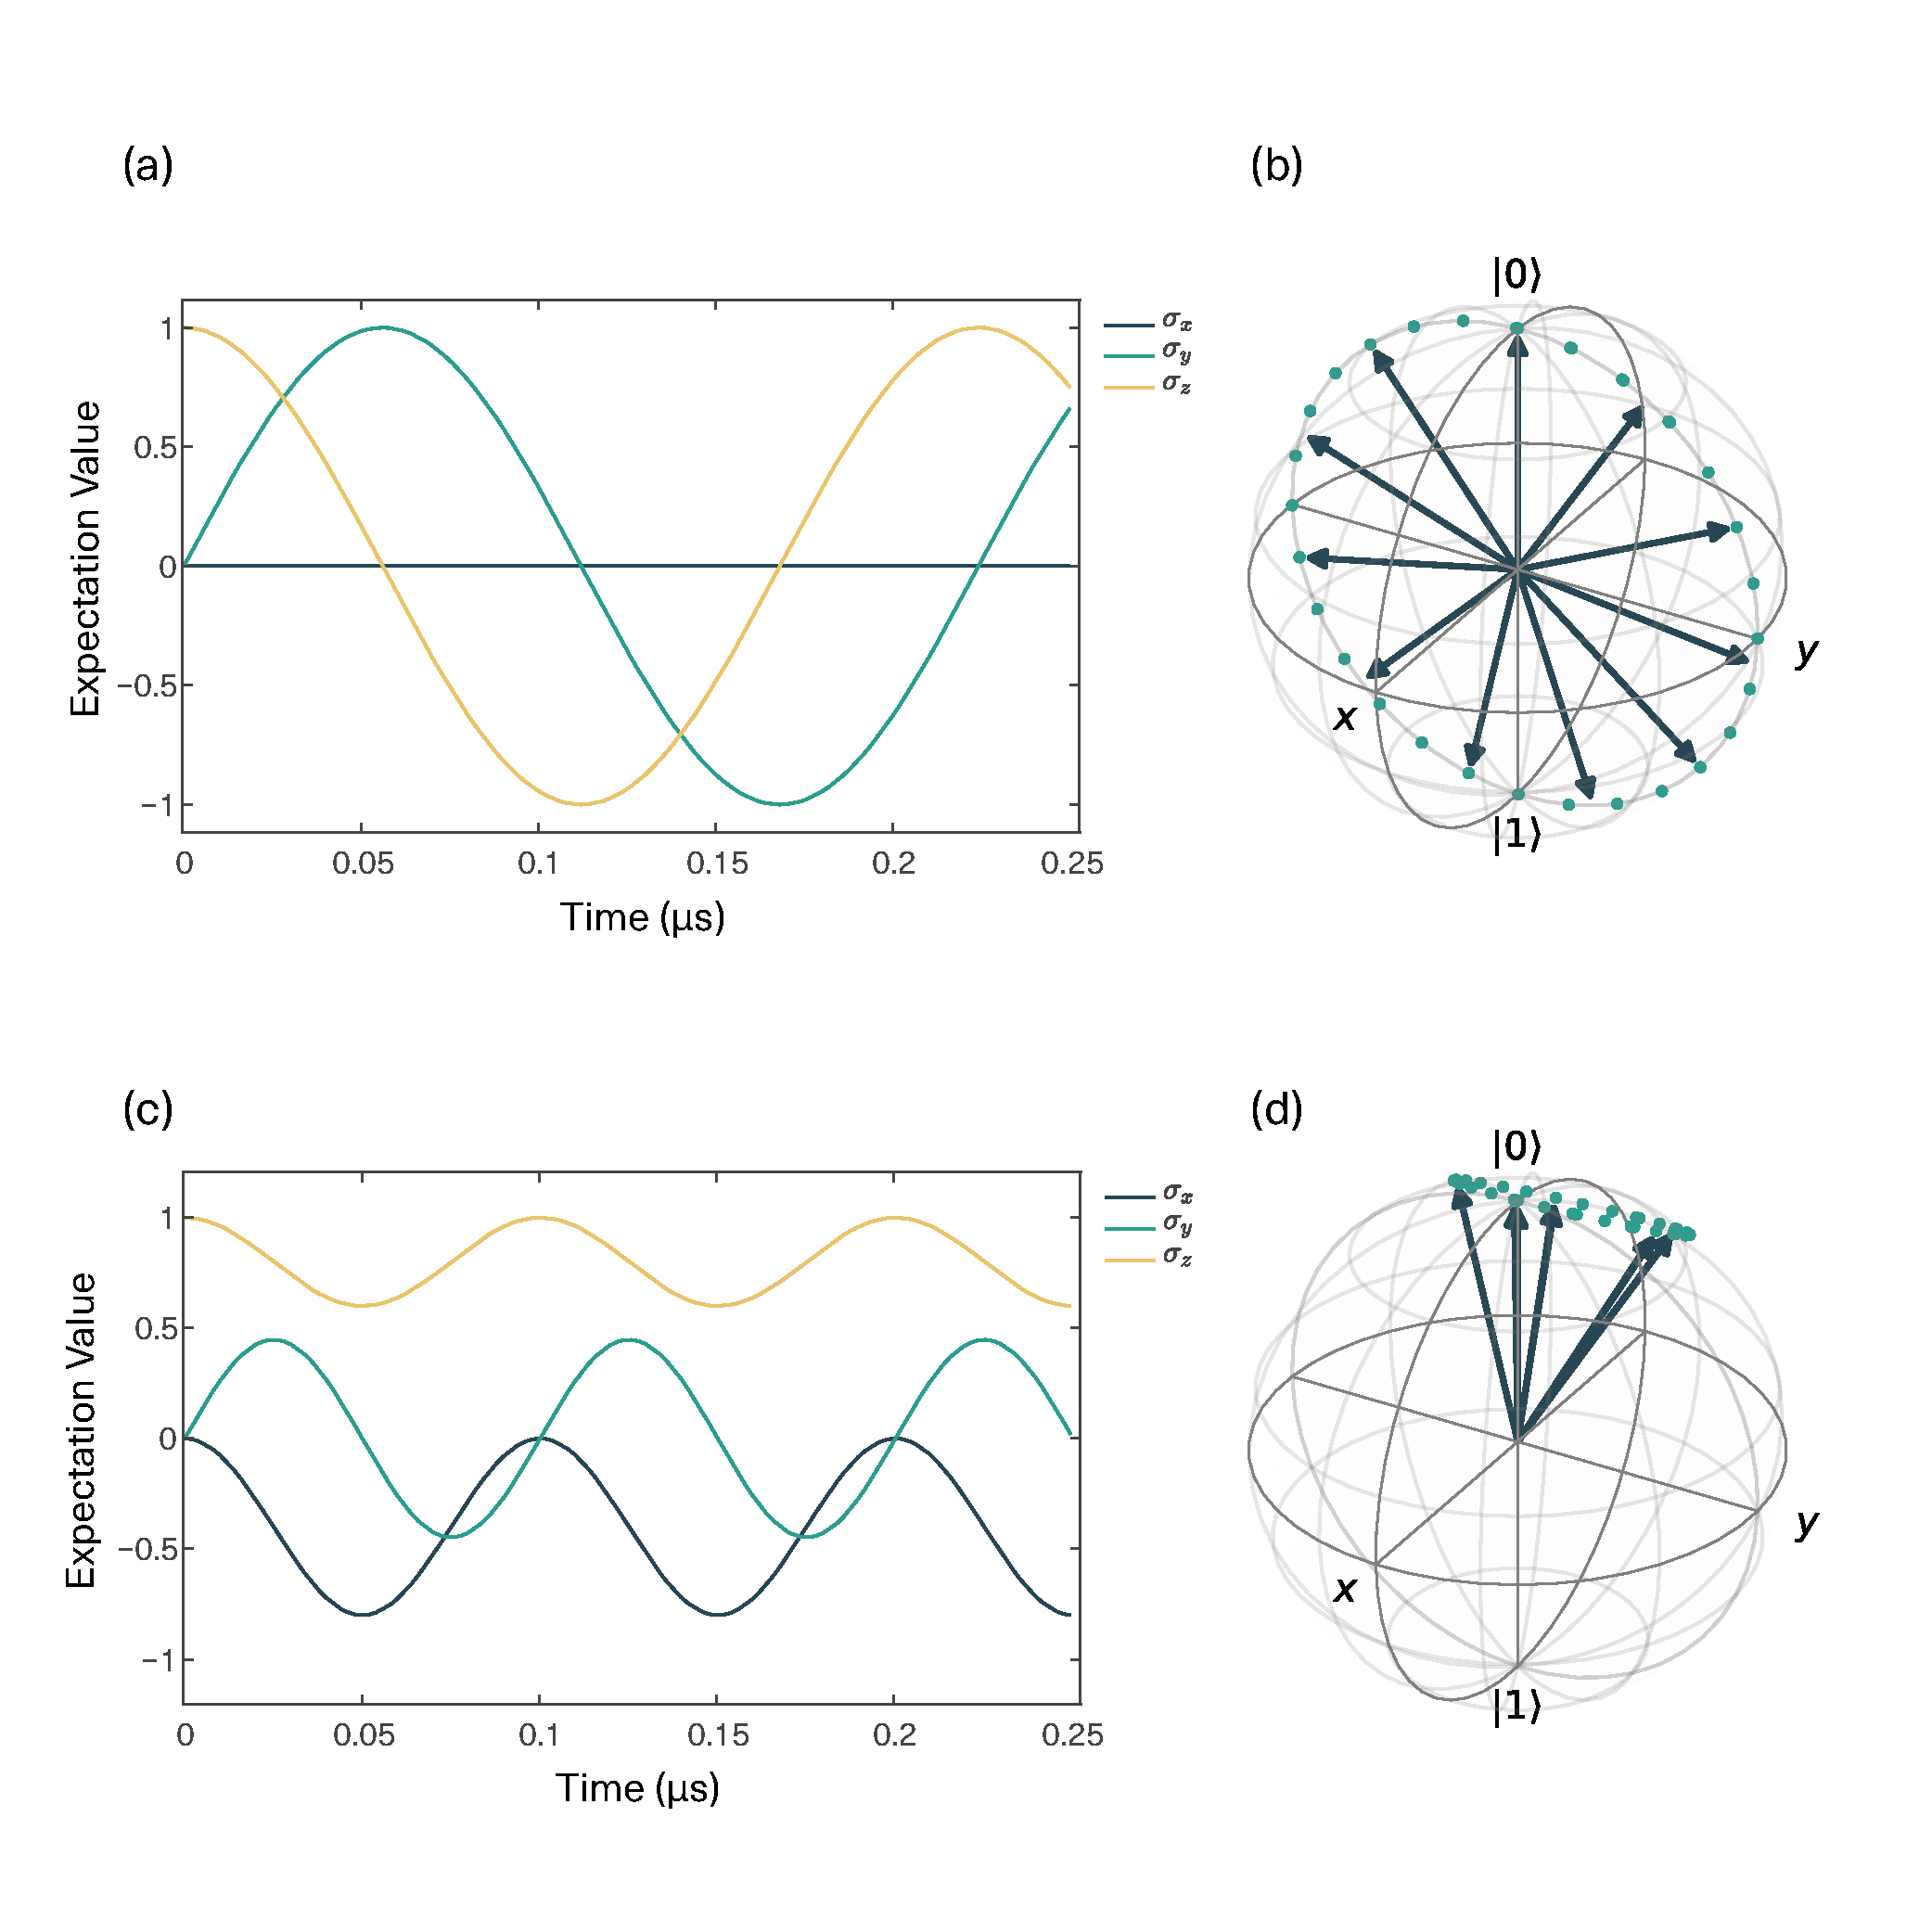
\includegraphics[width=\columnwidth]{/Plotting/Figs/rotating-frame.pdf}
  \caption[Qubit evolution under a an oscillating magnetic field in the rotating frame]{Figure showing qubit evolution under application of an oscillating magnetic field $B_1$, transformed into the rotating frame. In the on resonance case, where the frequency of the $B_1$ field is equal to the Larmor precession frequency of the $B_0$ field, (a) and (b) show the evolution of the expectation values of the Pauli matrices ($\sigma_x, \sigma_y$ and $\sigma_z$) and the state dynamics on the Bloch sphere respectively. (c) and (d) show the same figures for the case of off-resonance excitation, where the $B_1$ frequency is $0.5\%$ lower than the Larmor precession frequency.}
  \label{fig:rabi-dynamics}
\end{figure}

\subsection{Pulsed Electron Spin Resonance}
The processes described above show how a spin can be controlled via the application of magnetic fields, one, $B_0$, splits the electron spin states in energy whilst a second $B_1$ can be used to control the electron spin state. In practice, the process of controlling and measuring the spin states of electron is known as \emph{Electron Spin Resonance} (\textbf{ESR}) or equivalently \emph{Electron Paramagnetic Resonance} (\textbf{EPR}). There are two broad categories of ESR, continuous wave ESR (CW-ESR) and pulsed ESR. Typically, ESR is performed on large ensembles of electron spins, meaning that the behaviour of these spins is somewhat classical in nature as their individual magnetic moments $\mathbf{\mu}$ sum to produce an overall magnetic field vector $\mathbf{M}$.

CW-ESR refers to the process of detecting spin-transitions through the application of a constant oscillating magnetic field to a sample of interest. This field is applied via a resonator and the reflection of this field from the resonator is measured. An external magnetic field is varied and the reflection monitored. Whilst holding the static $B_0$ field constant and varying the $B_1$ field frequency is equivalent in theory, the resonators used for the oscillating fields have narrow ranges of operation meaning that varying the $B_0$ field is much more practical. As the static magnetic field is varied, electron spin transitions may come on resonance with the applied oscillating field, causing less of it to be reflected. This can be detected and the spin transition characterised by its g-factor~\cite{Gere1959,Feher1959}. This form of ESR is not used extensively in this work.

Pulsed ESR does not apply constant $B_1$ fields but instead uses pulses to control spin orientation. As described above, pulse duration (or power) and phase can be varied to rotate the spin vector $M$ to any point on the Bloch sphere. These pulses are usually referred to by their phase the angle of rotation they produce in the spin. So a pulse of duration $\Omega t = \pi$ is termed a $\pi$-pulse and serves to rotate a $\ket{0}$ state to a $\\ket{1}$ state. A $\frac{\pi}{2}$-pulse would rotate a $\ket{0}$ state to a point on the $x-y$ plane of the Bloch sphere.

These pulses provide a means to control the spin states but to be useful for experiments the spin state must be detectable as well. This is done by making use of the precession of the spins in the static magnetic field $B_0$. As these spins precess in the magnetic field they produce a small amount of electromagnetic radiation, with an oscillation frequency equal to their Larmor precession frequency. This radiation can be detected via the resonator that applies the pulses. The amplitude of this radiation is determined by the projection of the precessing spin vector in the $x-y$ plane, so a $\ket{0}$ or $\ket{1}$ produces no signal, whilst a state on the edge of the Bloch sphere in the $x-y$ plane will produce a maximum signal.

In a perfect system, all spins measured in this manner would precess at the same rate and produce a constant signal based on their projection in the $x-y$ plane. However, due to sample imperfections and spacial inhomogeneity in the applied $B_0$ field, each measured spin will precess at slightly different rates. The upshot of this is that the spin signal, made up of multiple signals from many spins, will rapidy lose phase-coherence and the overall signal will go to 0 due to destructive interference between spins rotating with different relative phases. This process is aptly named \emph{dephasing}.

To counteract this, it is possible to use a sequence of pulses to reverse this loss of phase coherence. Whilst many pulse sequences exist the simplest is the spin-echo or Hahn-echo sequence \cite{Schweiger,hahn1950}. This pulse sequence starts with the spin state at $\ket{0}$, where no dephasing occurs, a $\frac{\pi}{2}$ pulse is used to rotate the spin vector to the $x-y$ plane, at which point dephasing begins immediately causing the spin signal to decay. This decaying spin signal is known as \emph{Free Induction Decay} and can be measured to determine the spin state. It is typically not as the sensitive detection equipment used to measure the low-power spin signal can be damaged by high power control pulses, which can remain in the resonator for a short time after the pulse application. Instead the spin ensemble is allowed to dephase in the $x-y$ plane for an amount of time $\tau$ after which a $\pi$ pulse is applied, causing the spin ensemble to invert. The spins now experience the $B_0$ field in reverse and the dephasing they experienced is also reversed. Provided the inhomogeneities that cause the dephasing are constant in time, the spins will rephase after an additional time $\tau$ has ellapsed, causing a brief spike in their signal known as a spin echo. A schematic of this is shown in figure~\ref{fig:hahnechoseq}. A Hahn echo sequence represents the simplest of a broader class of pulse sequences known as \emph{Dynamical Decoupling} or \textbf{DD} sequences, which can be used to protect a spin ensemble or qubit against a variety of different sources of noise.

\begin{figure}
  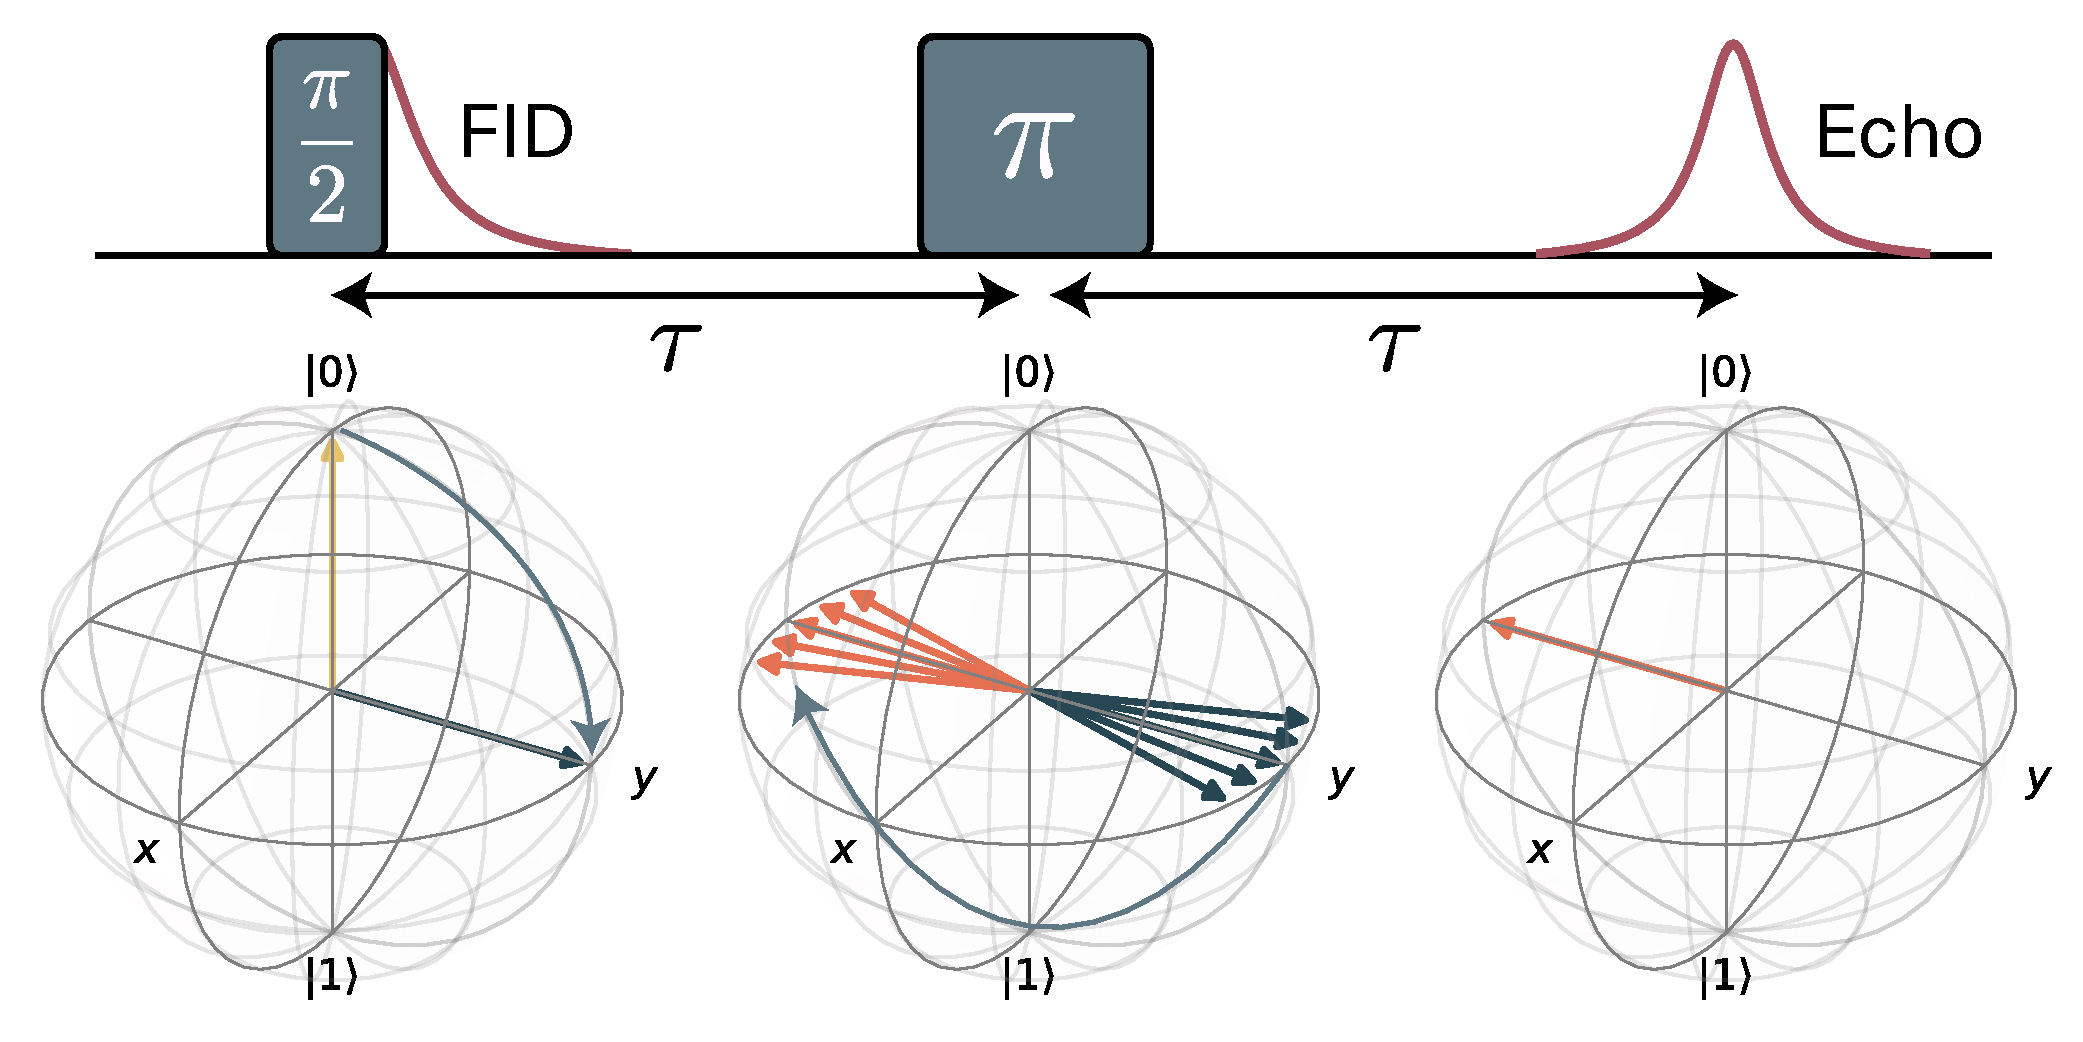
\includegraphics[width=\columnwidth]{/Plotting/Figs/hahn-echo-seq.pdf}
  \caption[Hahn echo sequence and bloch sphere]{Figure showing Hahn Echo sequence and its impact on an ensemble of spins on the Bloch sphere. The pulse sequence is shown above, starting with a $\frac{\pi}{2}$ pulse to take the $\ket{0}$ state into the $x-y$ plane. This then begins to dephase resulting in the rapid loss of signal - observed as the Free Induction Decay or FID. Next a $\pi$ pulse inverts the dephased spins after time $\tau$, causing them to experience a reversed magnetic field and to begin to rephase. After they rephase for another period of $\tau$ their signals interfere constructively once more and the characteristic echo is observed in the signal.}
  \label{fig:hahnechoseq}
\end{figure}

\subsection{Relaxation and Decoherence}

The process of dephasing, described above, introduces the concept of spin ensembles and their loss of phase coherence. This process of dephasing is part of a set of processes by which the ESR signal of an ensemble of spins might be lost or changed over time without control input. Broadly, these processes fall into the categories of \emph{relaxation} or \emph{decoherence} \cite{Schweiger}. Relaxation refers to the processes by which an ensemble of spins disturbed from thermal equilibrium returns to that equilibrium, its timescale is usually referred to as $T_1$. Decoherence refers to the irreversible loss of phase coherence and its timescale is referred to as $T_2$. Dephasing, the reversible loss of phase coherence is characterised by $T_2^*$. Although these processes are understood typically from the point of view of spin ensembles, they have analogous processes when single spins are addressed as well. Relaxation is the process of a qubit returning to its ground state after a certain amount of time. Decoherence is the process of a qubit losing internal phase coherence: the rate at which a superposition state will decay into a maximally mixed state with no quantum nature~\cite{Nielsen:2011:QCQ:1972505}.

\subsubsection{Spin Lattice Relaxation}

The spin relaxation process is most easily understood as the phenomenon that a spin prepared in some state on the Bloch sphere will eventually 'relax' back to the $\ket{0}$ ground state. Spin lattice relaxation is the dominant relaxation process for electron spins in silicon and is caused by the absorption or emission of phonons from the spin into the silicon lattice. From a more intuitive perspective, vibrations in the lattice cause fluctuating magnetic fields that mediate the energy transfer between the spins and the lattice.

As a phonon-mediated process, the dominant determiner of the spin lattice relaxation rate is the temperature of the lattice. There are three main spin-lattice interactions that can cause spin relaxation: \emph{direct, Raman} and \emph{Orbach}~\cite{Schweiger,Orbach1961,Castner1962}.

The direct spin lattice relaxation process is simply the case where the spin absorbs a phonon with frequency equal to the energy of the spin transition. The efficiency of this process is dependent on the phonon and vibrational mode density at the spin transition frequency and temperature, so scales with both. The exact dependence is material specific but at the high magnetic field limit can be approximated by:

\begin{equation}
  T_1 \propto B_0^{-4}T^{-1}
\end{equation}

The direct process is not typically the dominant relaxation process for spins in solids at typical temperatures (>4~K) as maximum phonon density is typically at significantly higher frequencies than the spin transition frequencies. This means that less efficient processes will dominate as more phonons are available to mediate the transition.

The first of these is the two-phonon \emph{Raman} process, whereby the spin first interacts with a phonon of significantly greater energy, $\omega_p$ than the spin transition frequency $\omega_0$. This excites the spin to a virtual excited energy state, before the spin decays back to its ground state by emitting a phonon of energy $\omega_p + \omega_0$. The virtual nature of the energy level allows all phonon energies to mediate this process. The dependence is:

\begin{equation}
  T_1 \propto T^{-9}
\end{equation}

This process is dominant for donors in silicon between 4~K and 10~K.

The final significant process for donor relaxation is the \emph{Orbach} two-phonon process. This is similar to the Raman process but involves the spin being excited to a real energy level rather than a virtual one by a resonant phonon. This process is dependent on the available excited states for the spin, which is donor dependent, and has an exponential dependence:

\begin{equation}
  T_1 \propto e^{-\Delta E / k_b T}
\end{equation}

This Orbach process is dominant in silicon donors at temperatures > 10~K. A schemtic showing the three spin lattice relaxation processes is shown in figure \ref{fig:relaxationprocs}.

\begin{figure}
  \centering
  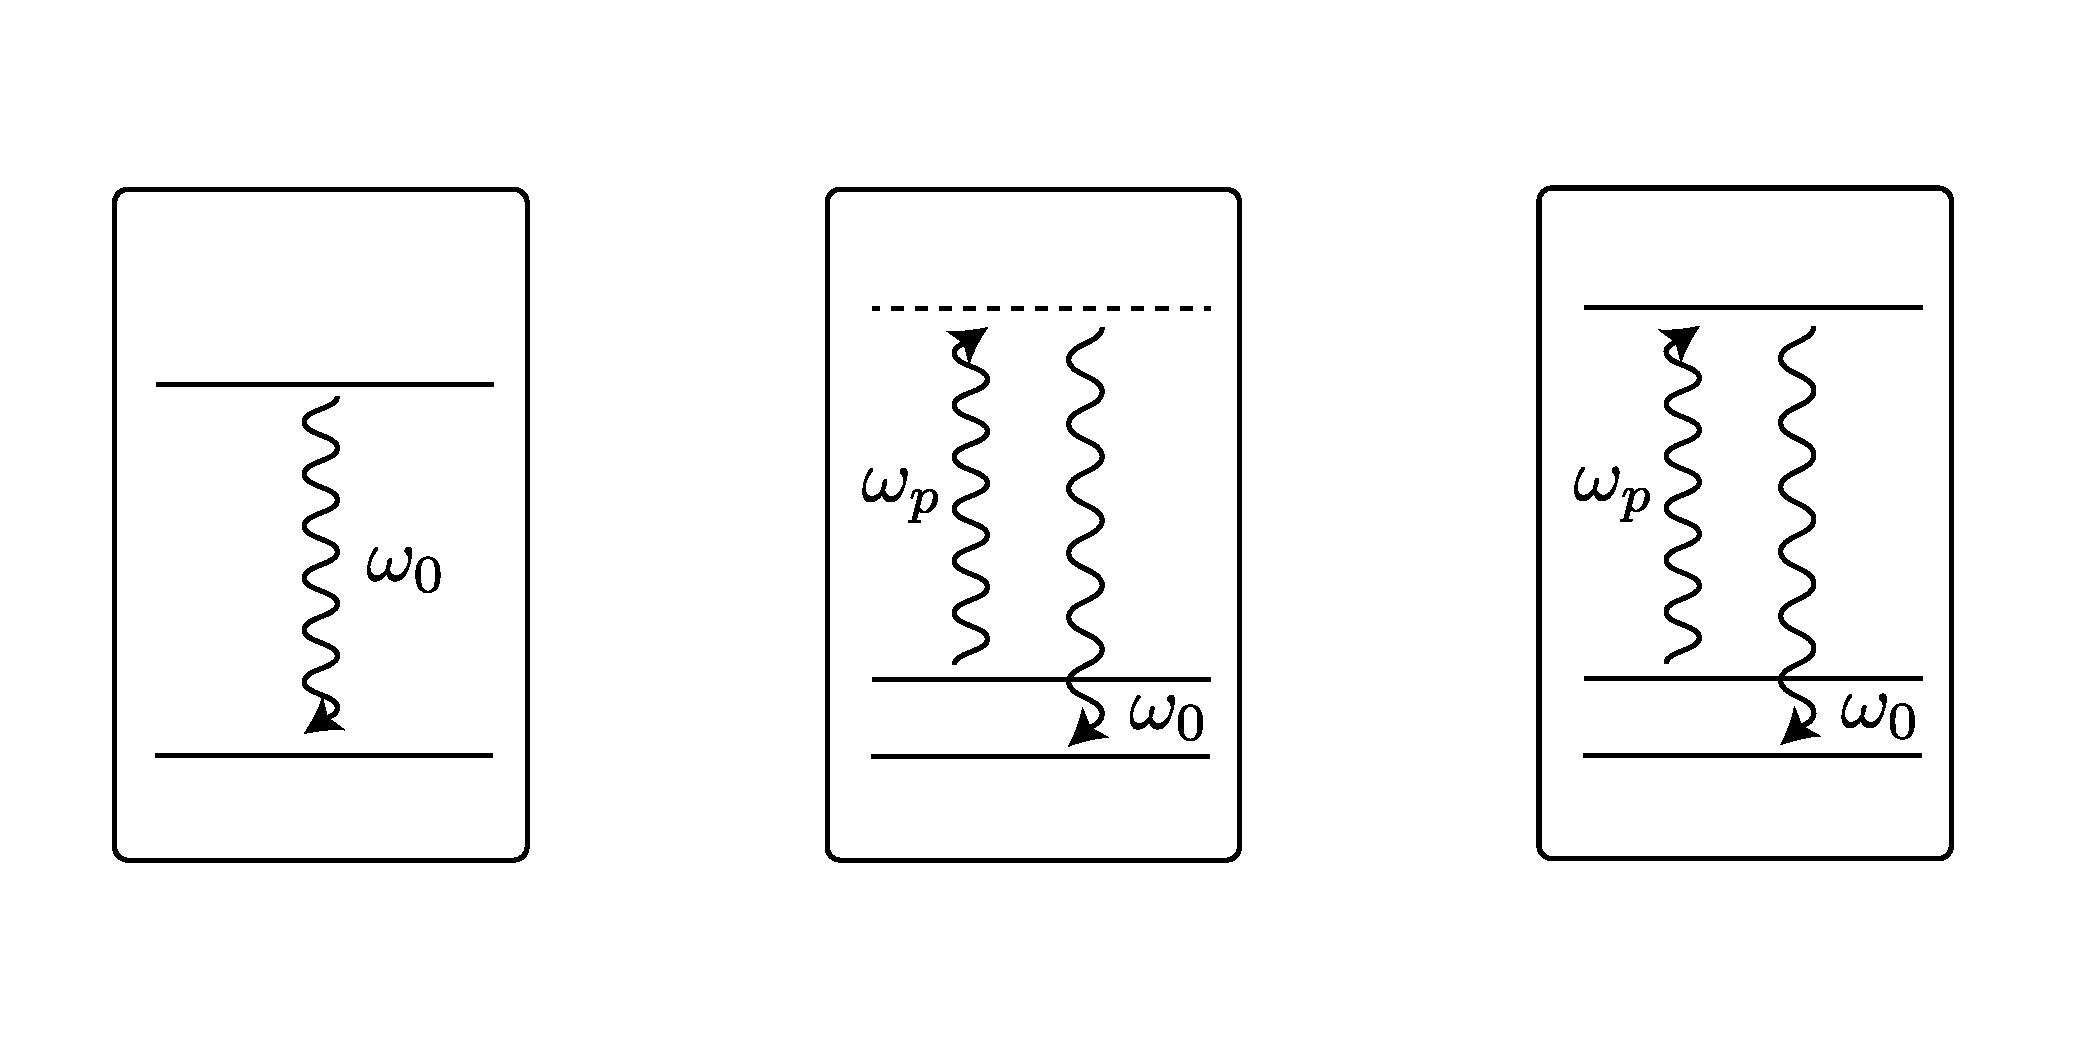
\includegraphics[width=\columnwidth]{/Plotting/Figs/relaxation-processes.pdf}
  \caption[Relaxation processes]{Figure showing simple schematic of the three spin-lattice relaxation processes: \emph{direct, Raman} and \emph{Orbach}. The direct process is dominant below 4~K and involves resonant absorption or emission of a single phonon, the Raman process dominates between 4~K and 10~K and involves non-resonant excitation by a phonon to a virtual energy level before emission of a phonon during relaxation from that energy level. Finally the Orbach process is a resonant two-phonon process requiring excitation to a real energy level before relaxation via phonon emission.}
  \label{fig:relaxationprocs}
\end{figure}

\subsection{Decoherence}


% \subsubsection{Hahn Echo and Detection}
%
% In pulsed ESR the spins are detected via the electromagnetic radiation they emit when precessing in a magnetic field.
% This radiation is of the same frequency as the resonant control radiation (easily shown using equations \ref{eq:enSplit} and \ref{eq:larmor}).
% This emitted radiation can be demodulated with the control radiation giving a DC signal.
% In a perfectly homogeneous magnetic field all spins would precess at the same rate giving a constant DC signal. In reality however, all spins will precess at slightly different rates due to small, static differences in the magnetic field each experiences.
% So, following a $\pi/2$ pulse, the signal from the spins will rapidly decay as the ensemble of spins lose phase coherence.
% A technique, known as a spin or Hahn echo, to reverse this loss of phase was developed by Erwin Hahn in 1950 \cite{hahn1950}.
% This follows a $\pi/2$ pulse with a $\pi$ pulse after a set time interval, $\tau$.
% \textit{Static} magnetic field differences now act to reverse the loss of phase coherence.
% This results in a brief re-phasing of the spins following another interval $\tau$, detected as a rise and fall of a DC signal or an `Echo'.
% A cartoon of this sequence is shown in figure \ref{fig:HahnEcho}.
%
% \begin{figure}
% \centering
% 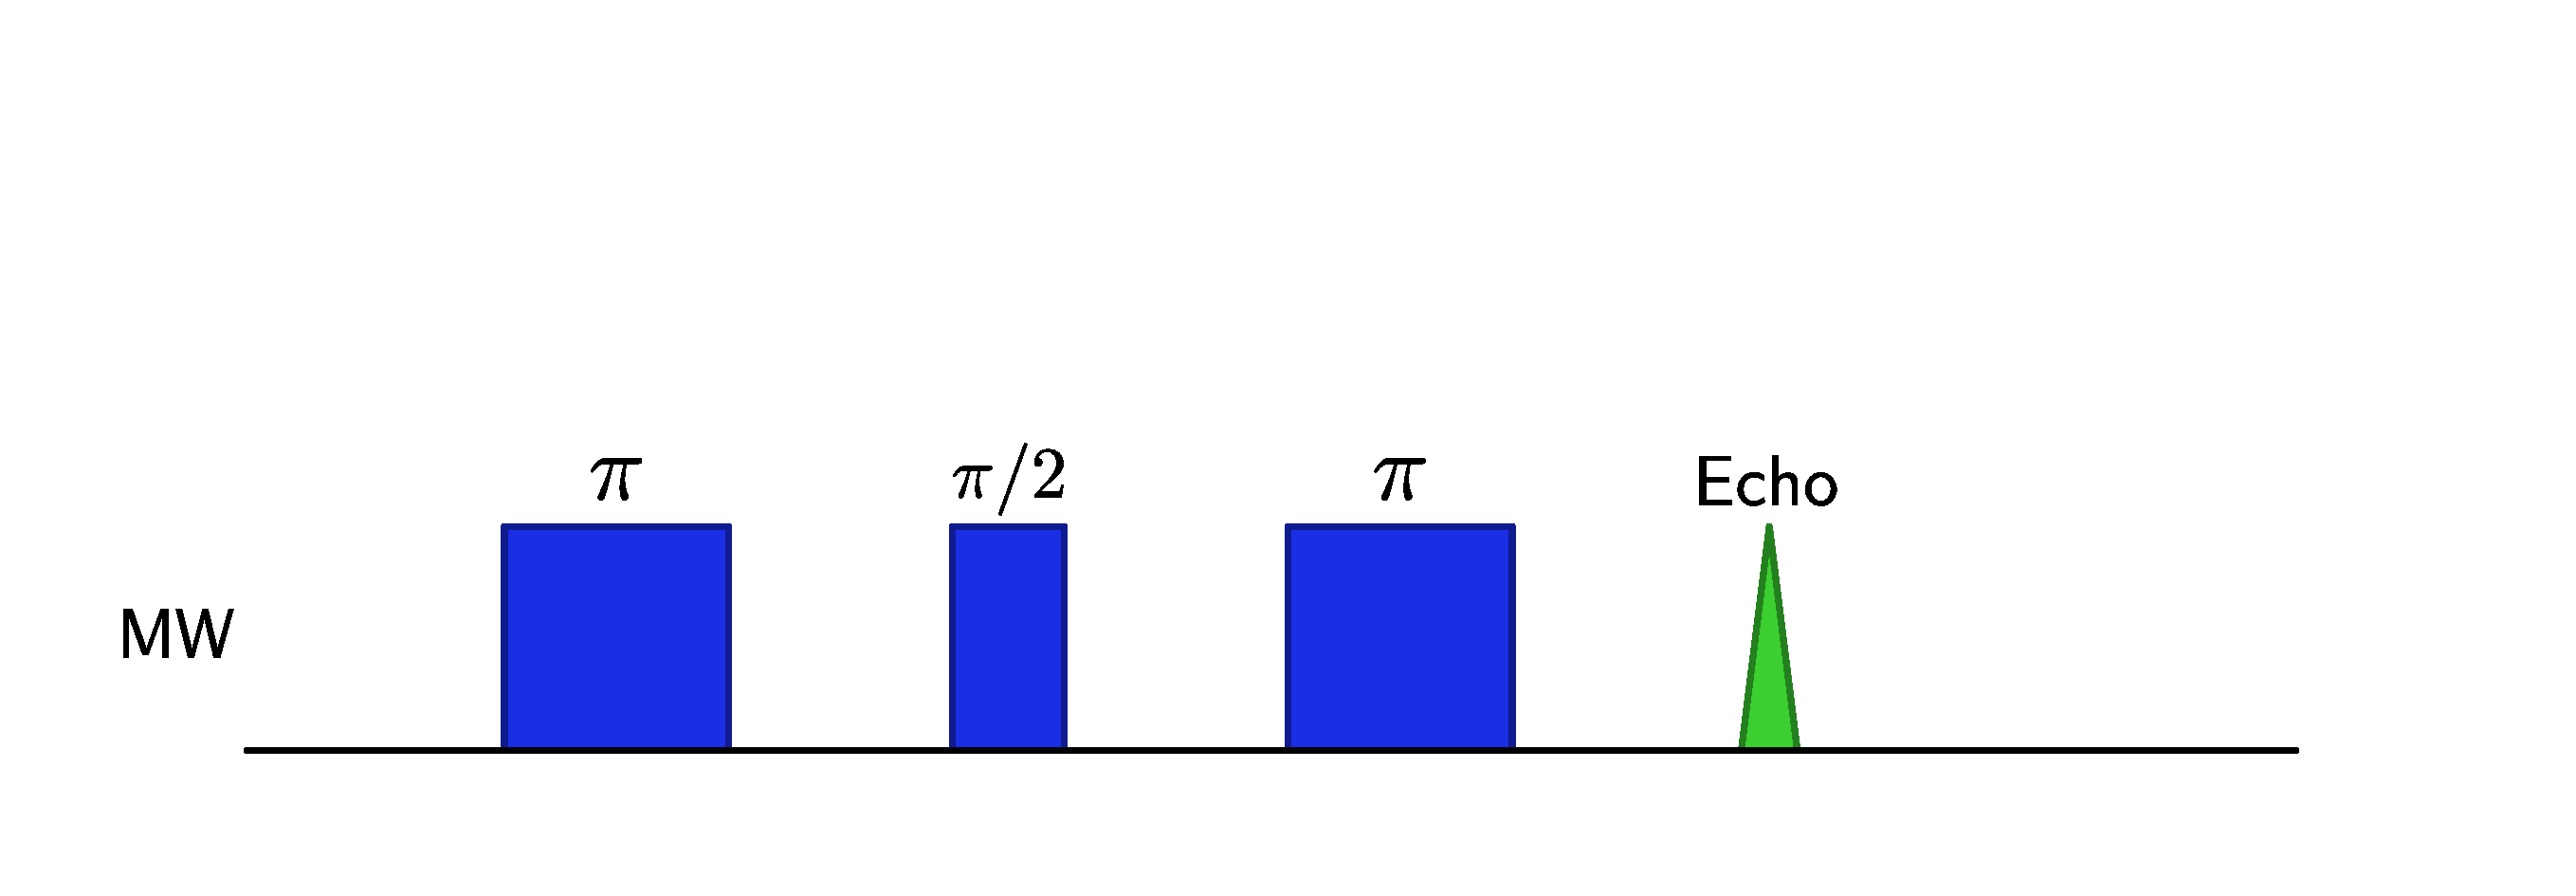
\includegraphics[width = \columnwidth]{Figures/hahnEcho.pdf}
% \caption[Hahn echo sequence]{Cartoon showing a Hahn echo pulse sequence. A $\frac{\pi}{2}$ pulse causes the spins to precess in the $x-y$ plane. Loss of phase coherence is reversed via a $\pi$ pulse following time interval $\tau$ and a signal is detected following another interval of $\tau$.}
% \label{fig:HahnEcho}
% \end{figure}
%
%
% \subsubsection{The Bloch Sphere}
%
% The control pulses produce a magnetic field that rotates at the same rate as the spins, meaning a fixed coordinate system can be defined.
% The rotation axis of the control pulses can be changed by varying their phase, for example a pulse of 0 phase is defined as a rotation about the $x$ axis whilst a pulse of $\pi/2$ phase is a rotation about the $y$.
% This allows control of the direction of the spin vector in 3-D space, with the $z$-axis defined by the static magnetic field.
% A qubit, the basic unit of a quantum computer, can be described as a point within a unit sphere, known as a Bloch sphere and shown in figure \ref{fig:blochSphere} \cite{Nielsen:2011:QCQ:1972505}.
% Clearly then, a single spin is an archetypal qubit: its eigenstates of $\ket{\uparrow}$ and $\ket{\downarrow}$ form the poles of the Bloch sphere.
% Microwave pulses of defined duration and phase enable the creation of an arbitrary linear superposition that allows the initialisation of any state on the surface of the Bloch sphere.
% In the case of ESR, however, a huge number ($10^{10}$) of spins is being addressed.
% Although this means that they do not represent a true qubit, measurements of ensemble properties give great insight into the behaviour of single spins.
% It is therefore prudent to establish the anticipated behaviour of the various potential spin qubit candidates using the comparatively simple experimental techniques of ESR before making the challenging step to single spin control and measurement.
%
% \begin{figure}
% \centering
% 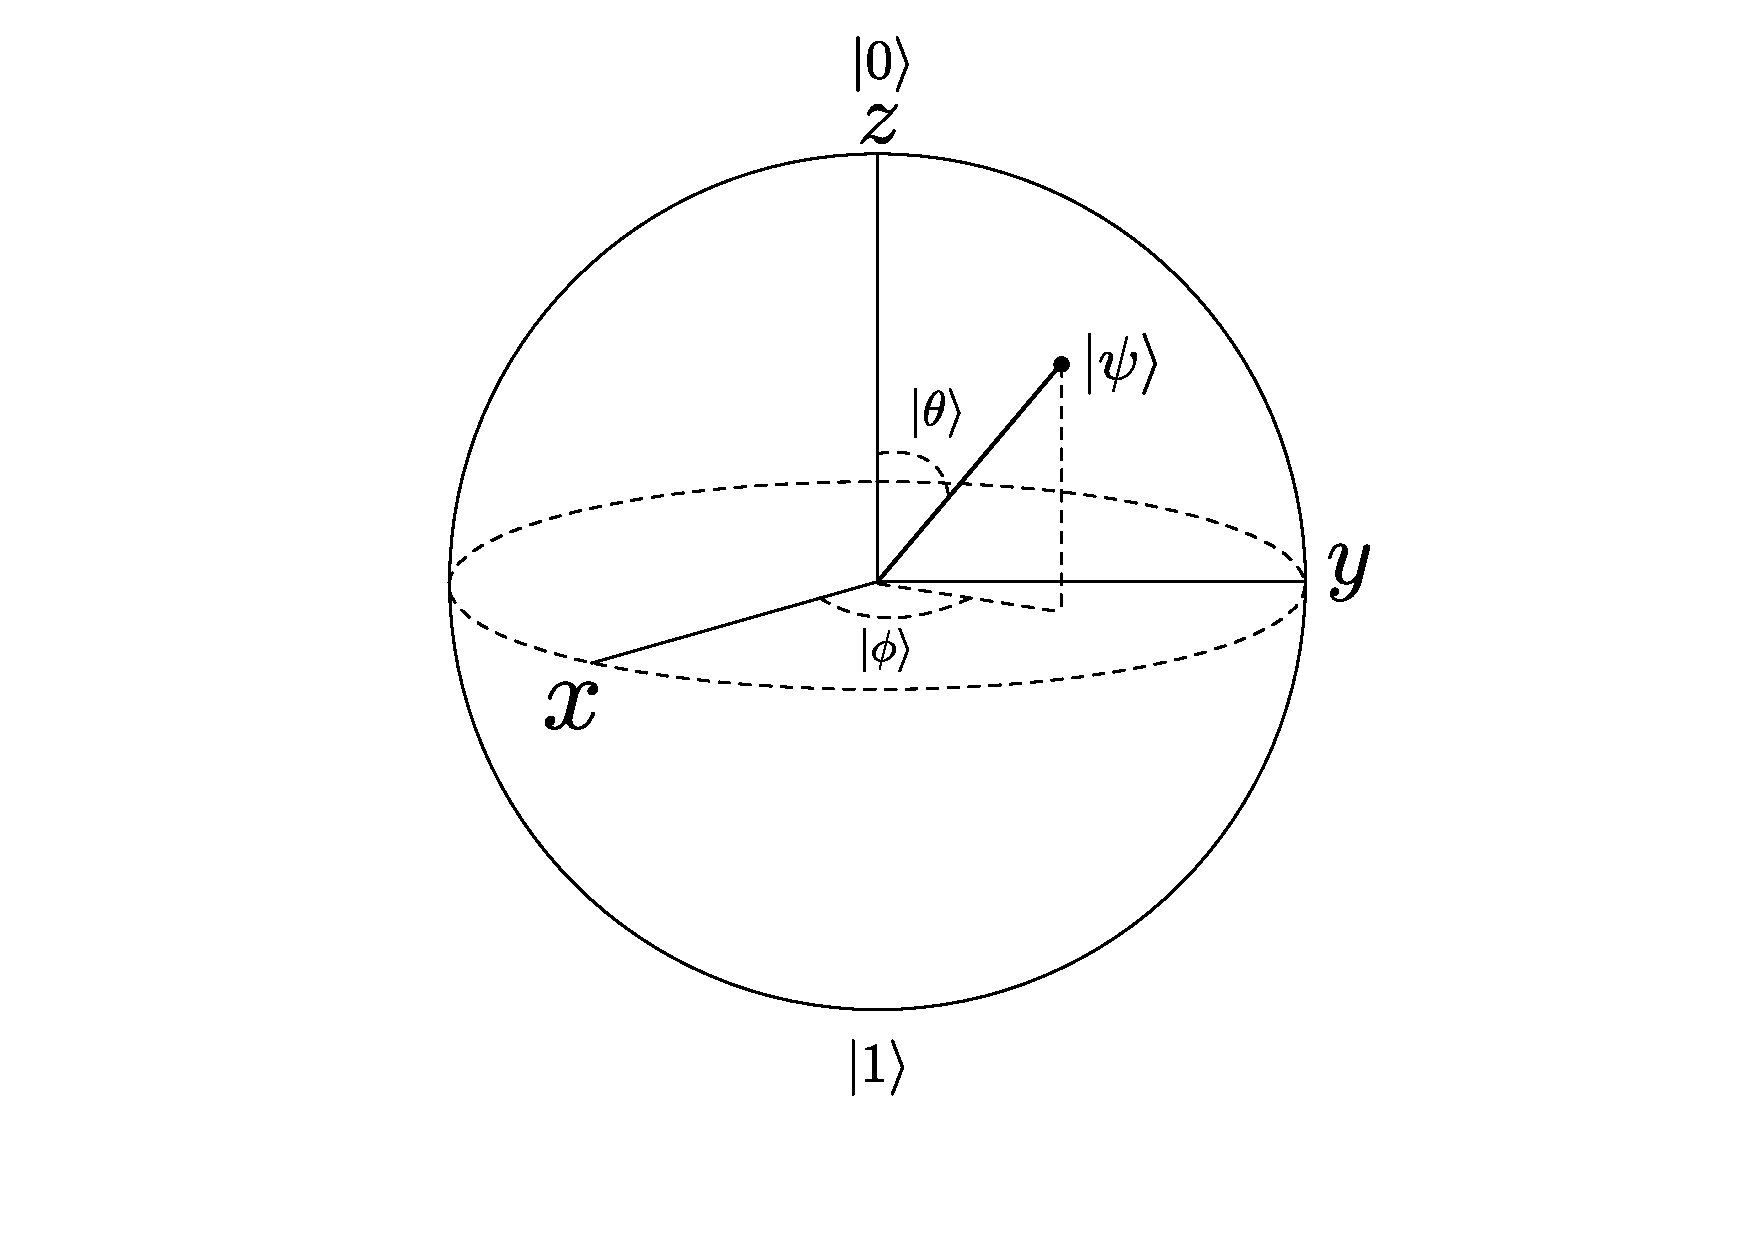
\includegraphics[width = 0.8\columnwidth]{Figures/blochSphere.pdf}
% \caption[Bloch Sphere]{Diagram of the Bloch sphere - the most common representation of a qubit. The poles of the sphere at $\pm z$ represent the $\ket{0}$ and $\ket{1}$ or $\ket{\uparrow}$ and $\ket{\downarrow}$ states. Any point on the surface of the sphere represents some linear superposition of these two states. The state vector of any point is given by: $\ket{\psi} = \cos{\theta/2}\ket{0} + e^{i\phi}\sin{\theta/2}\ket{1}$}
% \label{fig:blochSphere}
% \end{figure}
%
% \section{Donor States in Silicon}
%
% \subsection{The Hyperfine interaction}
%
% Discussion so far has focussed on single electrons in a magnetic field.
% The spins discussed in this thesis will be those of the electrons and nuclei of donors in silicon.
% For these spin states the situation is a little more complicated than the case of a free electron.
% For all the donors discussed here, there is a nuclear as well as electron spin.
% This introduces first an additional term in the Hamiltonian of the system due to the nuclear spin's Zeeman interaction with the magnetic field.
% On top of the separate Zeeman interactions there is an additional interaction between the nucleus and the electron, known as the hyperfine interaction.
% This term is due to the magnetic field of the electron interacting with the magnetic dipole moment of the nucleus.
% This strength of this interaction is proportional to the overlap between the electron and nuclear wavefunctions.
% The result of this is that it is preferential energetically for the electron and nuclear spins to be anti-aligned.
% A further term in the Hamiltonian is due to the nuclear quadrupole but this effect is small enough to be neglected in this treatment.
% These effects leave a Hamiltonian of the following form:
%
% \begin{equation}
% \label{eq:spinHam}
% \hat{H} = \mu_bg_eB_0\hat{S_z} + \mu_ng_nB_0\hat{I_z} + A \hat{S}\cdot\hat{I},
% \end{equation}
%
% where $\mu_b \text{\&} \mu_n$ are the Bohr and nuclear magnetons, $g_e \text{\&} g_n$ are the electron and nuclear g-factors, $\hat{S} \text{\&} \hat{I}$ are the electron and nuclear spin operators, and $A$ is the hyperfine interaction term.
% In general they hyperfine term is a tensor but due to the isotropic nature of silicon can be represented as a scalar here.
%
% \subsection{Spin Transitions}
%
% The electron spin is restricted to be $\pm \frac{1}{2}$, but the nuclear spin can take a much greater range of values.
% The nuclear spin of a phosphorus donor in silicon is $\pm \frac{1}{2}$, by contrast for a bismuth spin it can take the values $-\frac{9}{2}, -\frac{7}{2},...\frac{7}{2},\frac{9}{2}$.
% In the simple case of phosphorus this results in the four energy levels seen in figure \ref{fig:phosLevels}.
%
% \begin{figure}[t!]
% \centering
% \begin{subfigure}[t]{0.7\columnwidth}
% \centering
% 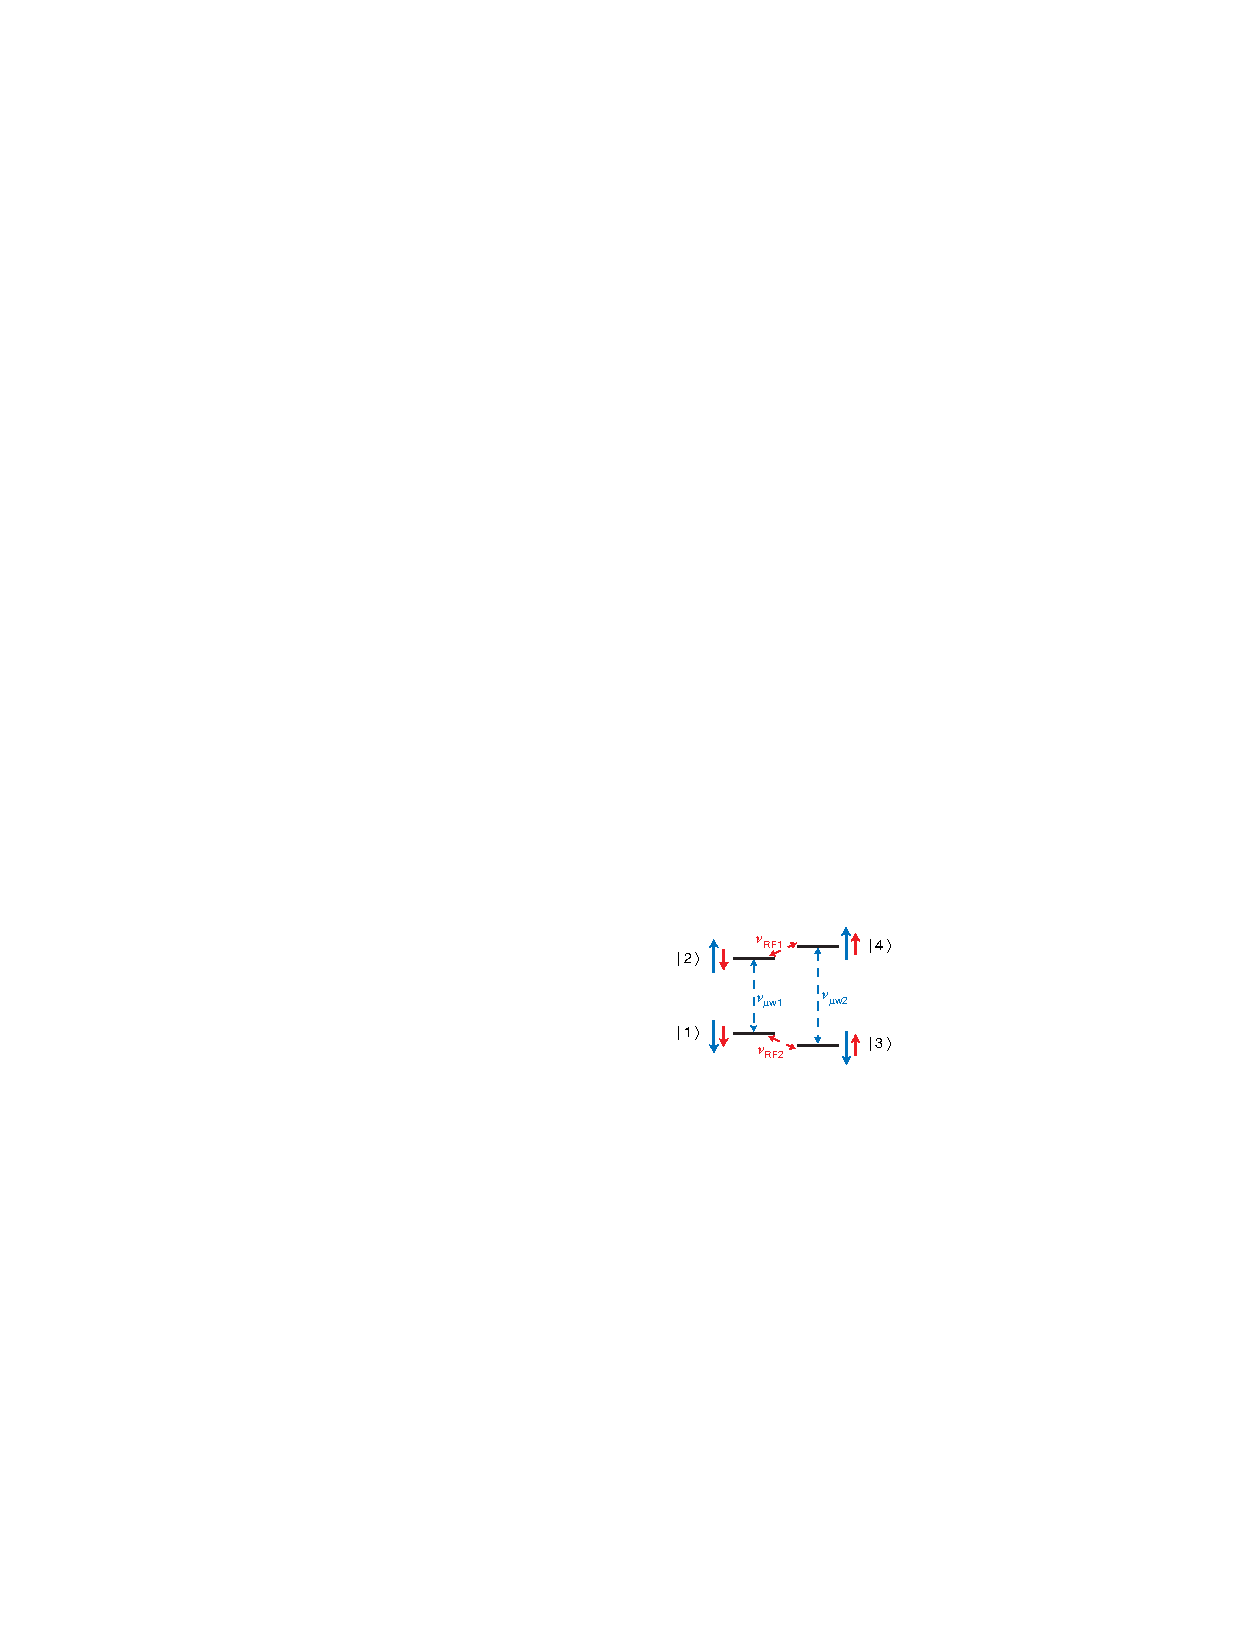
\includegraphics[width = \columnwidth]{Figures/phosphorus.pdf}{(a)}
% \end{subfigure}
% ~
% \begin{subfigure}[t]{0.7\columnwidth}
% \centering
% 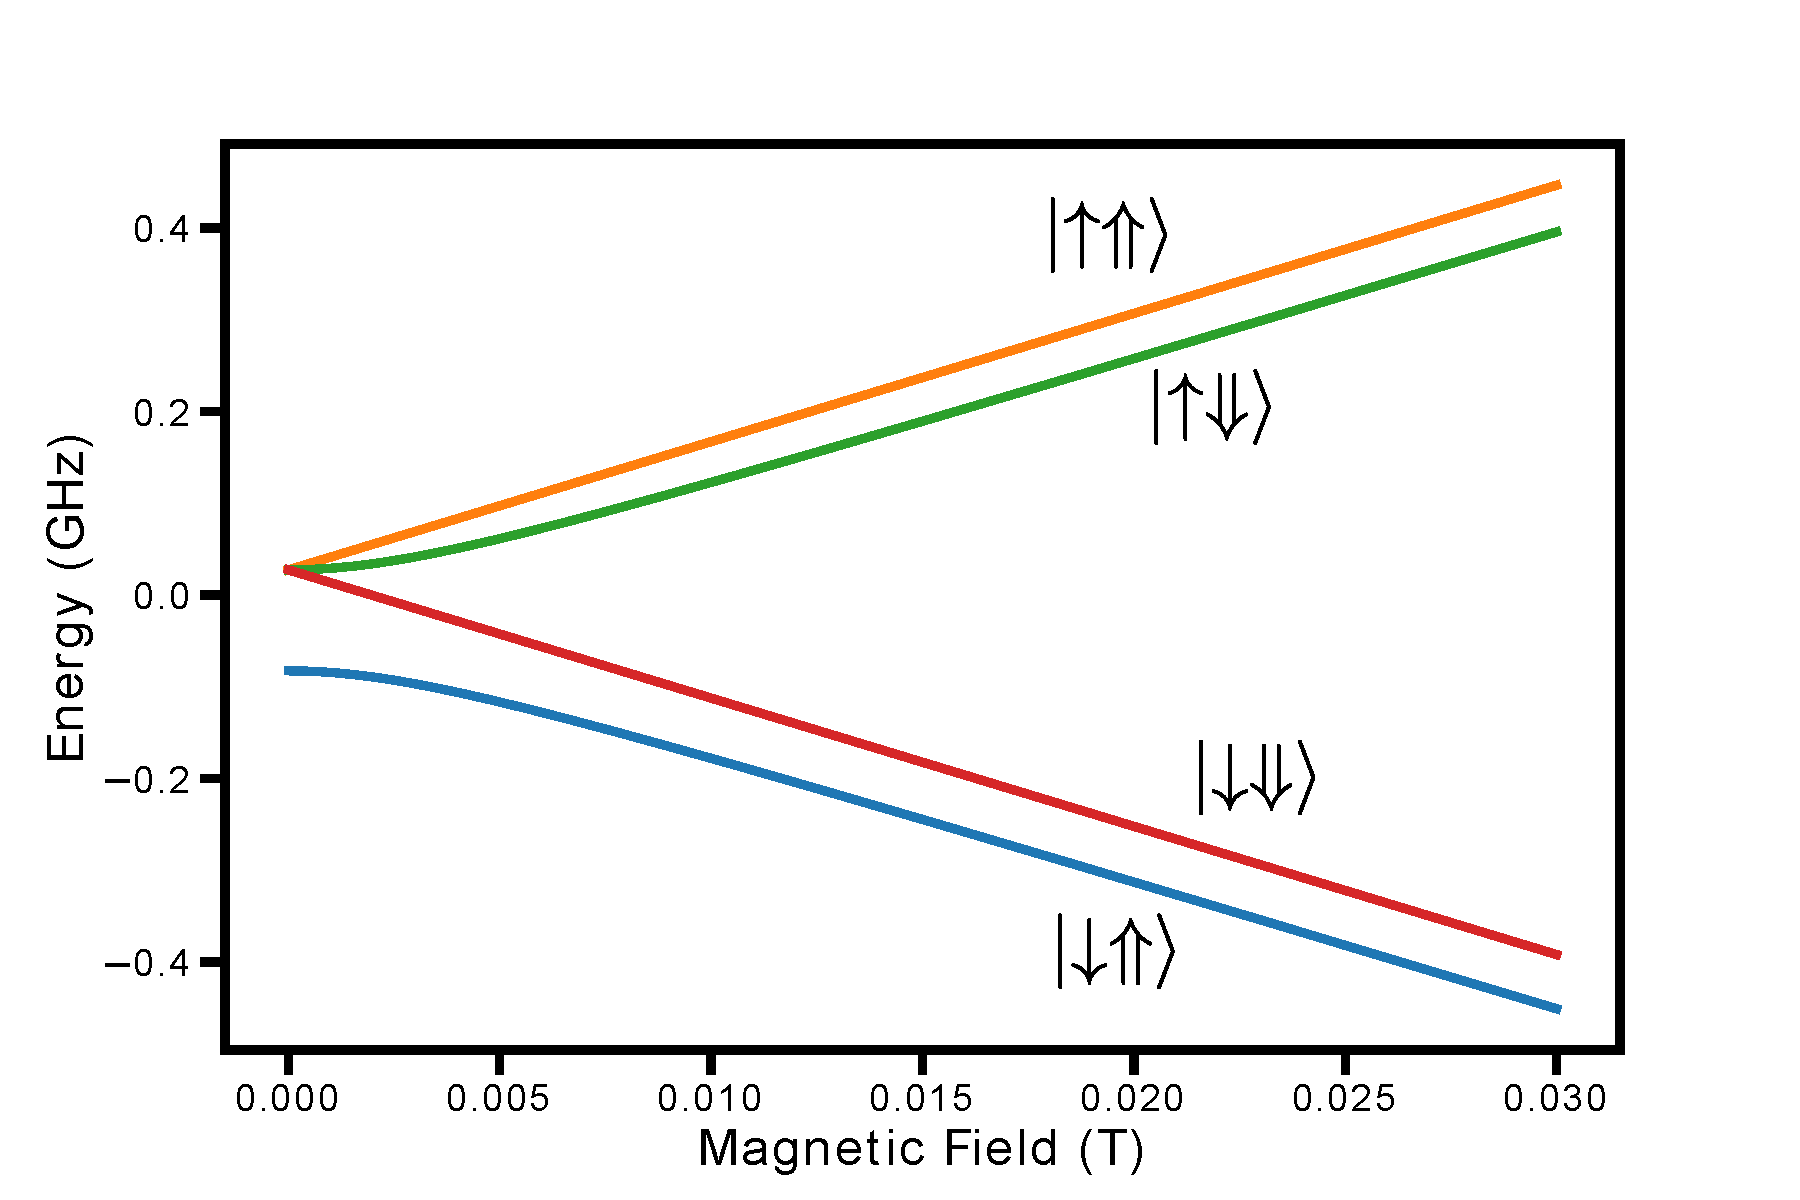
\includegraphics[width = \columnwidth]{Figures/fields.pdf}{(b)}
% \end{subfigure}
% \caption[Phosphorus energy levels and transitions]{Cartoon in a shows the relative energy levels for the different spin states of phosphorus in a high field environment. Note that in this case the electron Zeeman interaction dominates the hyperfine term which dominates the nuclear Zeeman term. b shows the simulated energies for each of the four possible states of the system.}
% \label{fig:phosLevels}
% \end{figure}
%
% For the more complex case of bismuth, instead of 4 possible energy levels there are 20.
% Not all transitions are possible - spins are changed by the absorption or emission of a photon, only allowing transitions where the total spin changes by $\pm1$.
% This means that only nuclear or electron spin can be flipped at once, not both.
% It should be clear that the transitions that involve an electron spin flip ( e.g. $\ket{\uparrow \Uparrow} \longrightarrow \ket{\downarrow \Uparrow}$) are significantly higher in energy than those involving a nuclear spin flip (e.g. $\ket{\uparrow \Uparrow} \longrightarrow \ket{\uparrow \Downarrow}$).
% At typical experimental magnetic fields ($\approx 0.3$ Tesla), the nuclear transitions are at frequencies of 10s of MHz, whilst the electron transitions are at $\approx 9.7$ GHz.
% In addition to their different energies electron and nuclear transitions have different strengths or Rabi frequencies.
% The electron spin transition is much stronger and occurs on the order of nanoseconds at typical pulse powers, with the nuclear transition being on the order of microseconds.
%
% \subsection{Relaxation Processes}
% \label{sec:relProc}
%
% For spins in silicon, three main relaxation or decoherence processes occur, causing the loss of information.
% \\
% \\
% \textbf{Dephasing}
% \\
% \noindent\rule{\columnwidth}{1pt}
% \begin{adjustwidth}{1.5cm}{}
% The first of these was briefly discussed above - dephasing - the time scale for the process is termed \textbf{$T_2^*$}
% This is the process by which an ensemble of spins loses phase coherence due to each spin experiencing a different static magnetic field.
% As was described above, this loss of information can be reversed by a Hahn echo sequence.
% \end{adjustwidth}
% \textbf{Relaxation} \newline
% \noindent\rule{\columnwidth}{1pt}
% \begin{adjustwidth}{1.5cm}{}
% The second process is known as relaxation and its time scale is termed $T_1$. A spin ensemble at a given temperature and magnetic field will have a Boltzmann distributed population across the available spin states defined by the magnetic field axis (i.e. across the eigenstates of the $\hat{Z}$ operator).
% The difference between higher and lower energy states is known as the polarisation of the ensemble.
% If this polarisation is reversed by a $\pi$ pulse, then on a time scale $T_1$ it will relax back to thermal equilibrium.
% As this process almost always involves interaction with the silicon crystal lattice it is also termed \textit{spin-lattice} relaxation.
% This process is strongly correlated with temperature and exact mechanisms will be discussed in the literature review section.
% \end{adjustwidth}
% \textbf{Decoherence}
% \\
% \noindent\rule{\columnwidth}{1pt}
% \begin{adjustwidth}{1.5cm}{}
% The third process, decoherence, occurs on the time scale $T_2$.
% This is similar to the dephasing process described above but is irreversible.
% Irreversible phase differences are caused by by inhomogeneous and \textit{time dependent} magnetic fields.
% Additional phase acquired due to a time varying magnetic field will not be reversed by a Hahn echo sequence as the field will act differently on the spin in the second half of the sequence.
% \end{adjustwidth}
%
% \section{Nitrogen Vacancy Centres in Diamond}
% \subsection{Diamond as a Material}
% \subsection{Energy Level Structure of the Nitrogen Vacancy Centre}
%
%
% \subsection{Summary}
%
% The theory discussed above gives a background to the topics that will be discussed in detail during the literature review section of this report.

% !TEX root = ../Thesis.tex

\chapter{Literature Review}
\label{chap:litRev}

Having introduced the background theory to the work discussed in this report, I turn to a more detailed examination of the literature surrounding it.
I begin with the various relaxation and decoherence processes for spins bound to donors in silicon.
First discussing the mechanisms by which these processes occur I shall then move on to the effect of illumination on these mechanisms.
Following this I shall move on the the stark shift of donor spins in silicon, including a brief introduction to the principle before an examination of previous work performed to characterise this effect in the various species of donor in silicon.


\section{Mechanisms of Relaxation and Decoherence}
\label{sec:mechrelax}
The concept of $T_1, T_2$ and $T_2^*$ time was introduced in section \ref{sec:relProc} as the characteristic relaxation, decoherence and dephasing times respectively.
I shall now focus on the established mechanisms by which these occur, looking mainly at relaxation and decoherence as these represent a permanent loss of information.

\subsection{Relaxation}

The relaxation time, $T_1$, determines the rate at which the polarisation of an ensemble of spins returns to Boltzmann equilibrium after being disturbed.
The first method of relaxation that should be considered is spontaneous emission: the emission of a photon into free space as the spin relaxes from excited to ground state.
For a magnetic dipole this rate is slow in normal circumstances - thousands of seconds or more \cite{schweiger2001principles,Baranov2017}.
Given that above millikelvin temperatures the rate of transverse relaxation for donor spins in silicon is significantly greater than this it can be neglected as a dominant mechanism.
\\
Spin-lattice relaxation occurs instead via the interaction with of the spin system with vibrations in the silicon lattice - phonons.
There are three different phonon-mediated processes that affect the relaxation rate of spin systems with transition frequency $\omega_s$, all of which are well described in a 1961 paper by Orbach \cite{VanVleck1940,Orbach1961}.
\\
\\
\textbf{Direct Process}
\\
\noindent\rule{\columnwidth}{1pt}
\begin{adjustwidth}{1.5cm}{}
The first of these is a \textbf{direct process}, whereby a single phonon with frequency equal to that of the spin transition (as given by equation \ref{eq:spinHam}) is emitted into the lattice.
This rate ($\propto 1/T_1$) is proportional to the phonon density at $\omega_s$ and varies with spin transition frequency and temperature as: $\omega_s^{-4}T^{-1}$.
\\
\end{adjustwidth}
\textbf{Raman Process}
\par\noindent\rule{\columnwidth}{1pt}
\begin{adjustwidth}{1.5cm}{}
Whilst this rate dominates at lower temperatures, $<10$k, at temperatures with $k_BT \gg \hslash\omega_s$, a two phonon Raman transition becomes more efficient.
As the maximum phonon density is at much higher frequencies than $\omega_s$, the spin first absorbs a phonon at $\omega_{\text{max}}$ before emitting a phonon with $\omega = \omega_{\text{max}} + \omega_s$.
This corresponds to the spin transitioning to a virtual energy level before rapidly transitioning back to the spin ground state.
For non-integer spin systems the rate due to this effect scales with temperature as: $T^{7}$.
\\
\end{adjustwidth}
\textbf{Orbach Process}
\\
\noindent\rule{\columnwidth}{1pt}
\begin{adjustwidth}{1.5cm}{}
The Raman process involves a virtual energy level so is an inherently off-resonant effect.
It is possible for the spin to transition to an actual excited state during the two phonon process.
This is known as an Orbach process and is more efficient than either process above.
It scales with temperature as: $\exp\left({-\Delta E/K_BT}\right)-1$.
\\
\end{adjustwidth}

\subsection{Decoherence}
\label{sec:litdecoherence}

At high temperatures the spin-lattice relaxation rate tends to be the dominant process for spins in silicon.
However, at temperatures below $\approx 10$k other factors become limiting.
In particular the decoherence or $T_2$ time becomes important.
This is the process by which the spins lose phase coherence irreversibly.
There are several mechanisms that contribute to $T_2$, detailed here .
\\
\\
\textbf{Spectral Diffusion}
\\
\noindent\rule{\columnwidth}{1pt}
\begin{adjustwidth}{1.5cm}{}
The first of these is spectral diffusion and its impact is largely dependent on the sample used.
In natural silicon samples there is a relatively high concentration of Spin-$\frac{1}{2}$ $^{29}$Si nuclear spins ($4.7\%$).
Due to the large extent of the donor electron wavefunction, it is highly probable that a given donor will experience a hyperfine interaction with one or more of these nuclei.
Although the large difference between the electron and nuclear gyromagnetic ratios prevents a state exchange or `flip-flop' interaction, nearby pairs of $^{29}$Si nuclei do have this interaction.
The rate of exchange is slow, ($\approx 100$Hz) and will cause a change in the hyperfine interaction with any nearby donor electrons.
This will cause the acquisition of phase differences between electrons over time.
As these changes are time dependent they are \textit{not} refocused by a Hahn echo sequence \cite{Wolfowicz2015a}.
In purified silicon samples this effect is reduced to the point that it is no longer the limiting factor in spin coherence.
\\
\end{adjustwidth}
\textbf{Instantaneous Diffusion}
\\
\noindent\rule{\columnwidth}{1pt}
\begin{adjustwidth}{1.5cm}{}
In the first experiments on spin coherence times on purified silicon, the increase in coherence time was found to be on the order 2 fold \cite{Gordon1958}.
The reason behind this limited increase was the high donor concentrations, leading to interaction between donors.
Spins that are close enough to interact with one another will experience slightly different magnetic fields and the random nature of donor distribution leads to this effect being inhomogeneous.
Once again, this will not be reversed by a Hahn echo sequence as two donors interacting with one another will both be flipped, meaning that the phase acquisition is unchanged.
This effect is dependent on the concentration of donors in a sample according to:

\begin{equation}
\frac{1}{T_{2}^{\text{ID}}} = C(2\pi\gamma_e)^2\frac{\pi}{9\sqrt{3}}\mu_0\hslash,
\label{eq:instDiff}
\end{equation}

where C is the donor concentration.
\\
\end{adjustwidth}
At concentrations useful for ESR techniques and at sufficiently low temperatures instantaneous diffusion will be a limiting factor in spin coherence times in almost all cases.
One technique employed by Tyryshkin \textit{et al}, open to ensemble based approaches such as ESR but not to single qubit control, is to use refocussing pulses of angle $<\pi$ in the Hahn echo sequence \cite{Tyryshkin2011}.
This effectively refocuses fewer spins during the Hahn echo sequence.
This reduces the signal but increases $T_2$ time as the effect of instantaneous diffusion is suppressed by addressed spins being on average much further apart.
At this point three further effects become limiting:

\begin{itemize}
\item \textit{Direct $T_1$ Flips}: only relevant at higher temperatures when $T_1$ is close to the intrinsic $T_2$, $>10$k. This is the process of a single donor flipping to its ground state, thereby destroying its coherence.
\item \textit{Spectral Diffusion from donors}: the limiting factor at low temperatures $<4$k, this process is similar to the spectral diffusion for $^{29}$Si spins. Nearby pairs of donors undergo spin exchange, causing any other nearby donors to experience a phase shift as their hyperfine coupling changes.
\item \textit{$T_1$ of Neighbouring Donors}: this process is important at intermediate temperatures, between $4$k and $10$k. At these temperatures direct $T_1$ flips are yet to dominate but $T_1$ flips of neighbouring donors can affect the magnetic field experienced by a central donor. This effect is known as $T_1$-type spectral diffusion.
This process was identified by Tyryshkin \textit{et al} as producing shorter than expected $T_2$ times when $T_1$ appeared to no longer be a limiting factor \cite{Tyryshkin2011}.
The decoherence rate as a function of $T_1$ induced spectral diffusion has a characteristic, stretched exponential of the form $\exp(-(2\tau/T_{SD})^2)$, with $T_2^{SD} = \sqrt[]{T_1}$.
\end{itemize}

The five key contributors to decoherence are shown in figure \ref{fig:decoherenceTypes}.
The key contributors to decoherence times are then:

\begin{itemize}
\item \textit{Temperature}: when $T_1$ is sufficiently short at high temperatures the $T_1$ of the donors will restrict $T_2$. At intermediate temperatures $T_1$ flips of neighbouring donors induces spectral diffusion, reducing $T_2$.
\item \textit{Sample Purity}: the concentration of $^{29}$Si spins in the silicon has a significant impact on $T_2$ due to spectral diffusion via nuclear spin flip-flop.
\item \textit{Donor Concentration}: the concentration of donors increases the rate of instantaneous diffusion, indirect flip-flop, direct flip-flop and $T_1$ type spectral diffusion.
\end{itemize}

With the mechanisms of decoherence addressed, I now turn to examine the effect of illumination on donor relaxation and coherence rates.

\begin{figure}
\centering
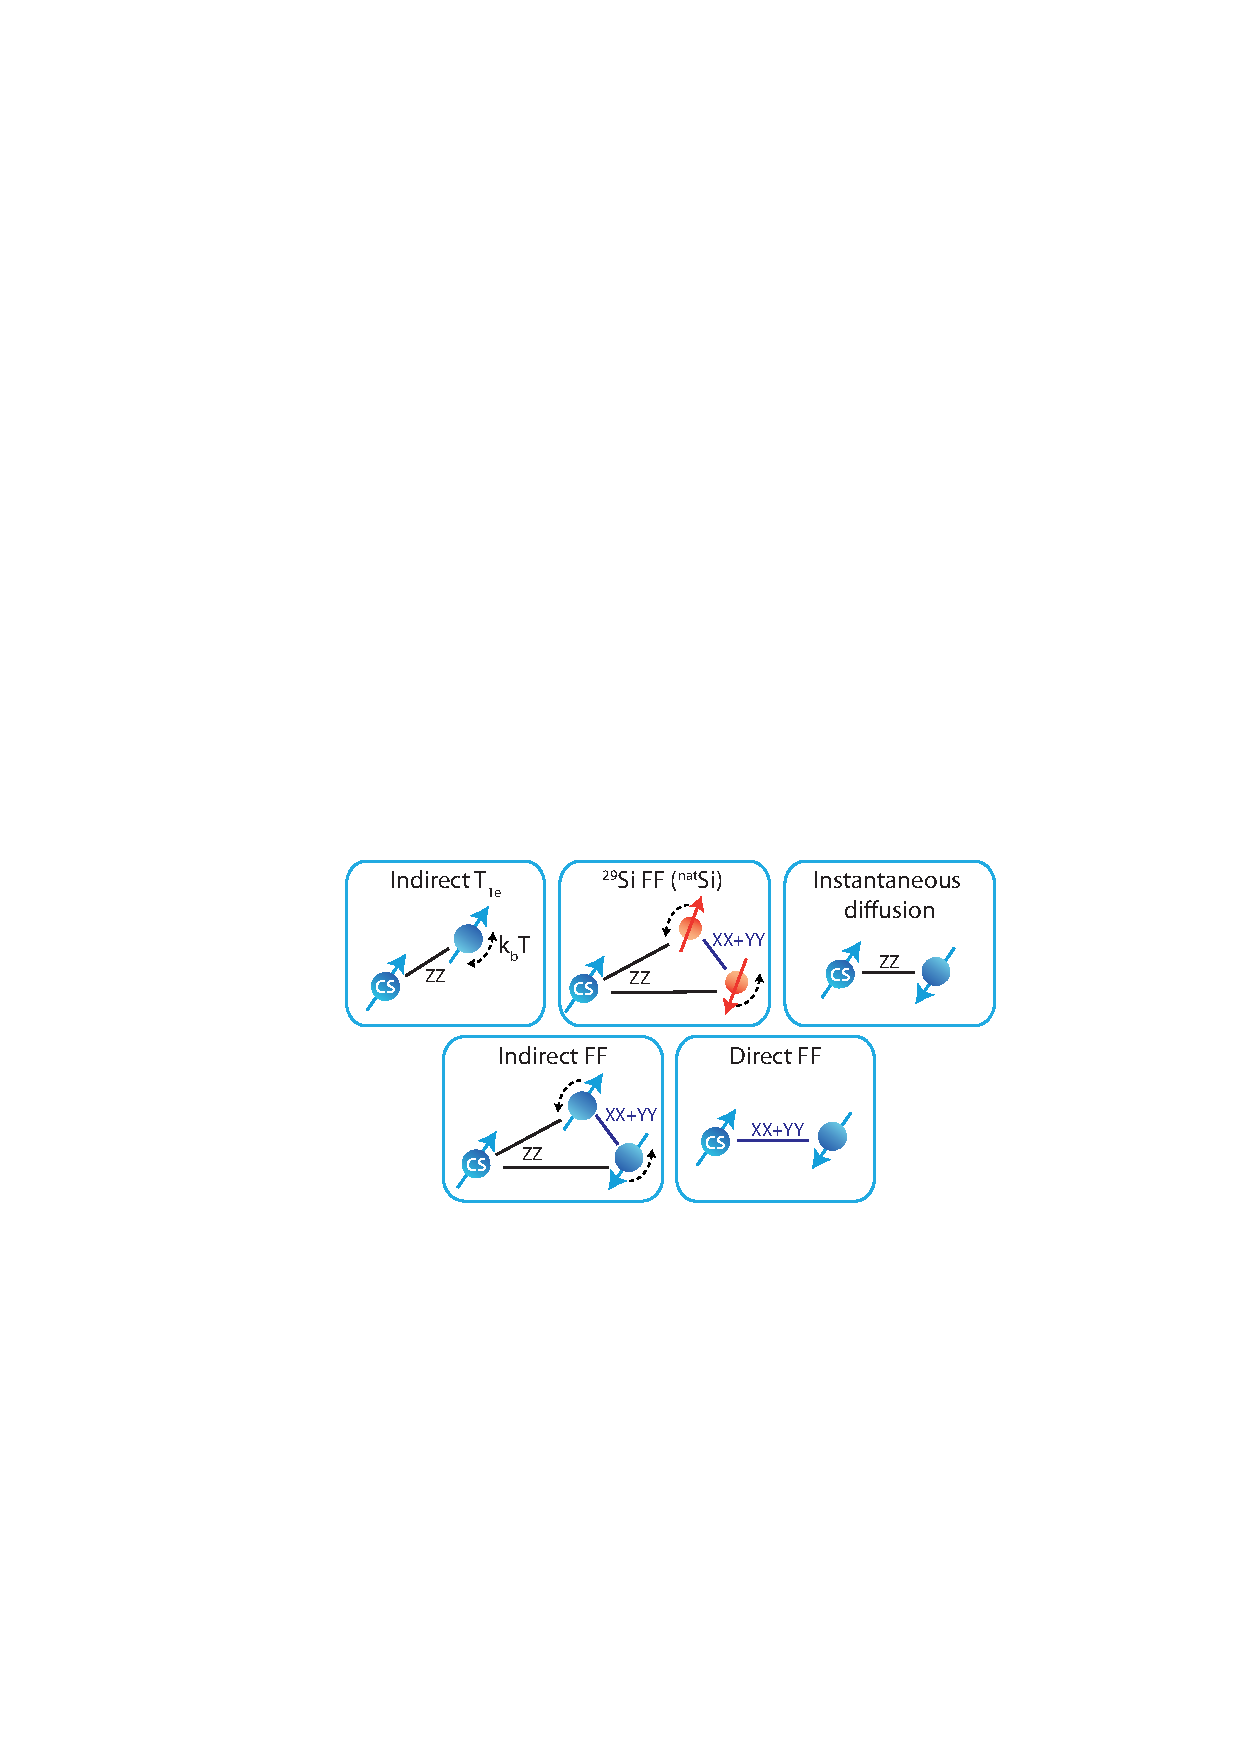
\includegraphics[width = \columnwidth]{Figures/decoherenceTypes.pdf}
\caption[Decoherence mechanisms in silicon]{Cartoon showing the five key types of decoherence mechanisms for donor electrons in silicon. Indirect $T_1$ is the relaxation of a neighbouring donor modulating the magnetic field at a central donor. Flip-flops of $^{29}$Si nuclear pairs modulating the magnetic field at the donor. Instantaneous diffusion is the inhomogeneous phase acquisition of donors due to different inter-donor spacings. Indirect flip-flop mechanism is similar to that involving $^{29}$Si nuclei but with pairs of donors. Direct flip-flop is state exchange between a central donor and a neighbour. Figure is taken from \cite{Wolfowicz2015a}.}
\label{fig:decoherenceTypes}
\end{figure}



\section{Illumination and Decoherence}

\subsection{Free Carriers and Decoherence}

The discussion above centred on the typical factors that affect coherence and relaxation times:  temperature, donor concentration and silicon purity.
One of the key questions addressed in this report is the impact of another factor on relaxation times: illumination.
Feher and Gere were among the first to examine this impact in their 1959 paper \cite{Gere1959}, analysed using CW ESR of phosphorus donors in silicon.
The key question that they examined is the impact of illumination wavelength on relaxation time, the results of which can be seen in figure \ref{fig:phosPhotFeher}.
The important result here is the sharp increase in relaxation rate as the photon energies exceed that of the silicon band gap, $\approx 1.12$eV.
As this energy is exceeded by the photons, free carriers are created in the silicon conduction band as electrons are promoted from the valence band.
These free carriers can scatter off the electrons bound to the phosphorus donors, causing them to relax via a state exchange.
Feher and Gere postulate two possible processes that could cause this relaxation: the first is direct scattering of a donor electron by a free electron, whilst the second is a two stage process.
They identify the second of these as dominant, due in the main to the low number of free electrons relative to donors in their experiments - $5\times10^6$ vs $7\times10^{15}$ - with each interaction requiring the subsequent relaxation of the conduction electron to the lattice.
The double spin exchange process does not involve the free electron changing spin, instead both the nuclear spin of the donor and the electron bound to it change spin state.
This removes the requirement that the conduction electron subsequently relax to the valence band, significantly increasing the rate of the process.
\\

\begin{figure}
\centering
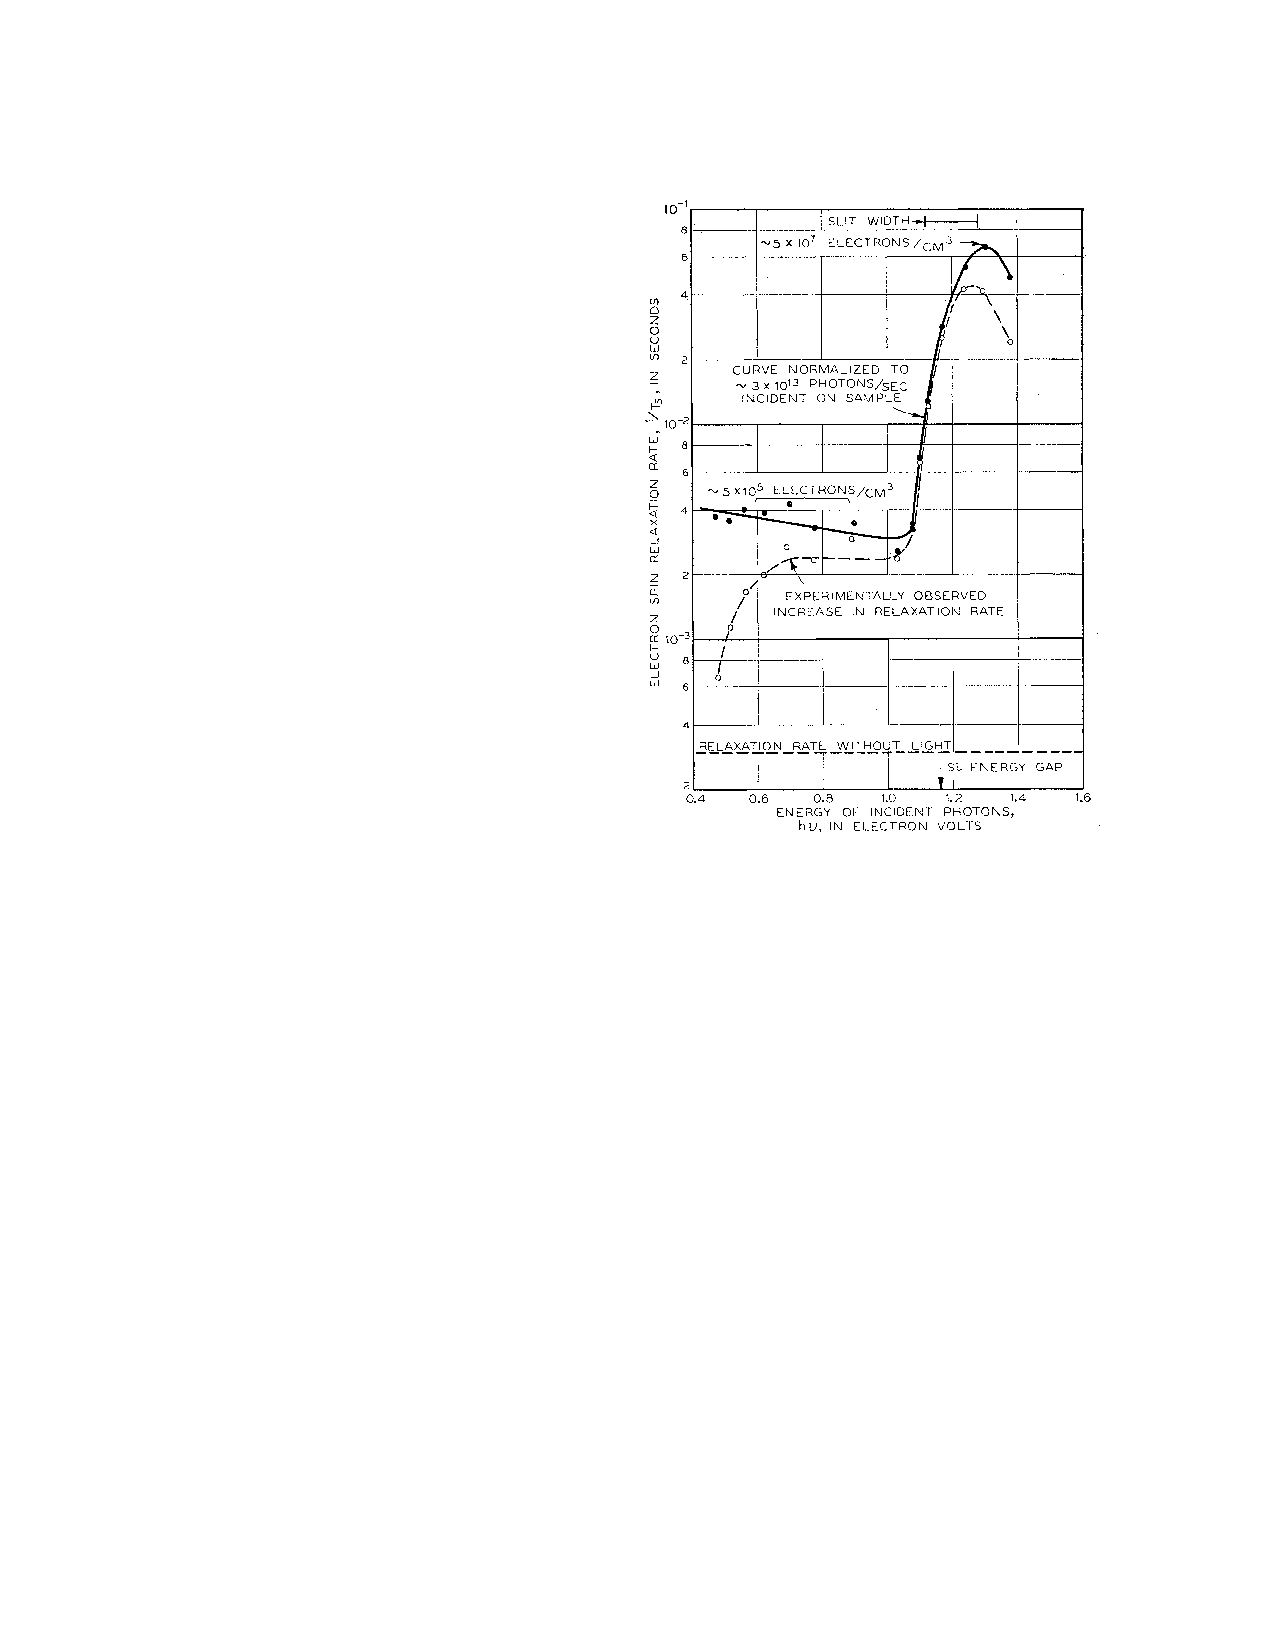
\includegraphics[width = 0.75\columnwidth]{Figures/photEngDep.pdf}
\caption[$T_1$ dependence on photon energy]{Graph from \cite{Gere1959} showing the measured dependence of relaxation time on photon energy. Notable is the sharp increase in relaxation rate for photon energies in excess of 1.10~eV. The main cause of this is that this is the energy of the photon band gap, meaning that free electrons are created in the silicon conduction band. These free electrons can then scatter off the electrons bound to donors in silicon, causing them to relax.}
\label{fig:phosPhotFeher}
\end{figure}

The work done by Feher and Gere was performed using only CW ESR, because of this their work addresses only the impact of laser illumination on $T_1$.
The key timescale for quantum computing is the coherence time, $T_2$, which must be examined using pulsed ESR.
Whilst $T_2$ time will ultimately be limited by $T_1$ a concern is that free carriers in the silicon conduction band will have an impact beyond this.
It seems obvious that the presence of these free carriers could alter the magnetic environment of the donors in a time-dependent and inhomogeneous fashion, potentially having a drastic impact on the coherence time of donors.
Examining the impact of illumination on decoherence times will be an important goal of this report.

\subsection{Heating and Decoherence}

A potential factor not addressed by Feher and Gere is the impact that heating could have on relaxation and by extension coherence times.
Although the number of free carriers produced by laser illumination will be significantly reduced as photon energies drop below the band gap, it is possible that heating could still have a significant impact.
Of particular note is the reduced heat capacity of silicon at low temperatures.
At room temperature heat capacity ($C_p^o$) is 19.1 J.mol$^{-1}$k$^{-1}$, but at cryogenic temperatures this is reduced by several orders of magnitude to approximately 0.004 J.mol$^{-1}$k$^{-1}$ at 8~K \cite{Desai1986,Niinikoski1986}.
Clearly then the potential impact of infra-red illumination is obvious - only a small conversion of incident photons to phonons in the lattice could potentially have a significant impact on the relaxation rates for donor spins.
Exploring this potential impact will be a central goal of this report.
\\
Having looked at some of the literature surrounding the questions of relaxation and decoherence of donors in silicon, I now move on to the stark shift of donors in silicon.

\section{The Stark Shift}
\label{sec:starkShiftLit}

\subsection{Introduction}

The Stark shift, at its simplest, is the modulation of the hyperfine coupling between electron and nuclear spins via electric fields.
The Stark shift was employed in Kane's original proposal as a means to control which qubits interact with an applied control pulse \cite{Kane1998}.
As well as the potential application for control of donor spins, the Stark shift presents a problem in the potential for electric field noise to cause decoherence of donor spins.
This impact may become particularly important for single donors close to electrical contacts where distances are short and so fields high.
Clearly then an understanding of the stark shift and its impact on donors is useful both from control and decoherence perspectives.
\\
An intuitive understanding of the stark shift is easily grasped: the electron's wavefunction extends over space and is concentrated at the donor nucleus.
This concentration determines the hyperfine coupling of the spin to the donor.
An electric field changes this wavefunction, effectively pulling it off the nucleus and changing the hyperfine coupling, as seen in figure \ref{fig:starkShift}.
This in turn changes the energy difference between the two spin states of the electron and modulates its precession frequency in a static magnetic field.

\begin{figure}
\centering
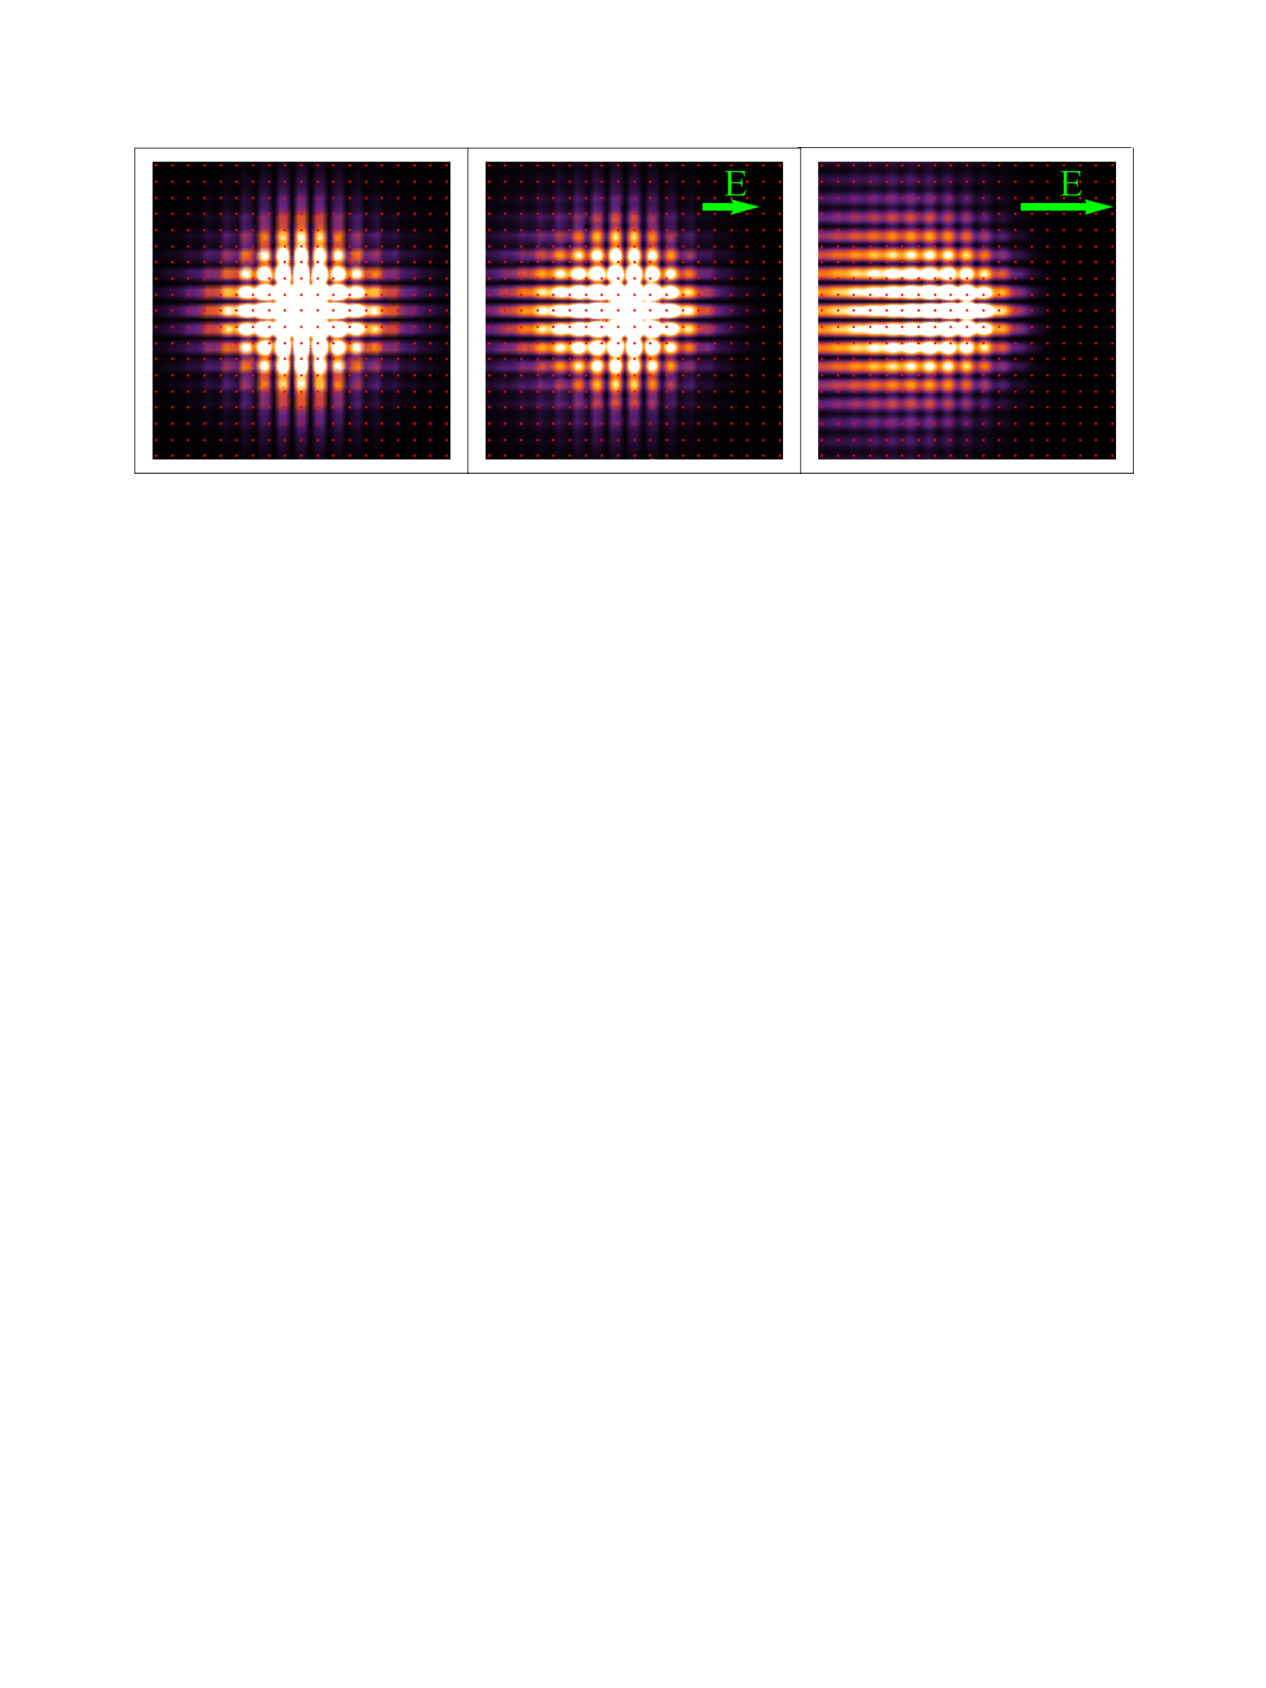
\includegraphics[width=\textwidth]{Figures/starkShift.pdf}
\caption[Electron wavefunction Stark shift]{Simulation showing the density of the electron wavefunction around a donor atom. Red dots represent lattice sites. As an electric field is applied the electron wavefunction is pulled off the central site, changing the strength of its interaction with the donor nucleus and therefore its hyperfine coupling. This shifts the frequency of the electron's spin transition and its precession rate in the magnetic field. Figure reproduced from \cite{Pica2014}.}
\label{fig:starkShift}
\end{figure}

\subsection{Theory}

A technical description of the Stark shift in most cases employs effective mass theory and here I follow the approach taken by Pica \emph{et al} \cite{Pica2014}.
This treats the donor system as if it were a hydrogen atom with a different mass embedded in a silicon lattice as opposed to a vacuum.
This is done by replacing the electron's vacuum mass with its effective mass in the silicon and modifying the vacuum permittivity with the dielectric constant of silicon \cite{Wolfowicz2015a}.
The conduction band of silicon has 6 minima - usually termed 'valleys' - situated in the $\pm x, \pm y, \pm z$ directions and close to the edge of the Brillouin zone, as seen in figure \ref{fig:siliconband}.

\begin{figure}
\centering
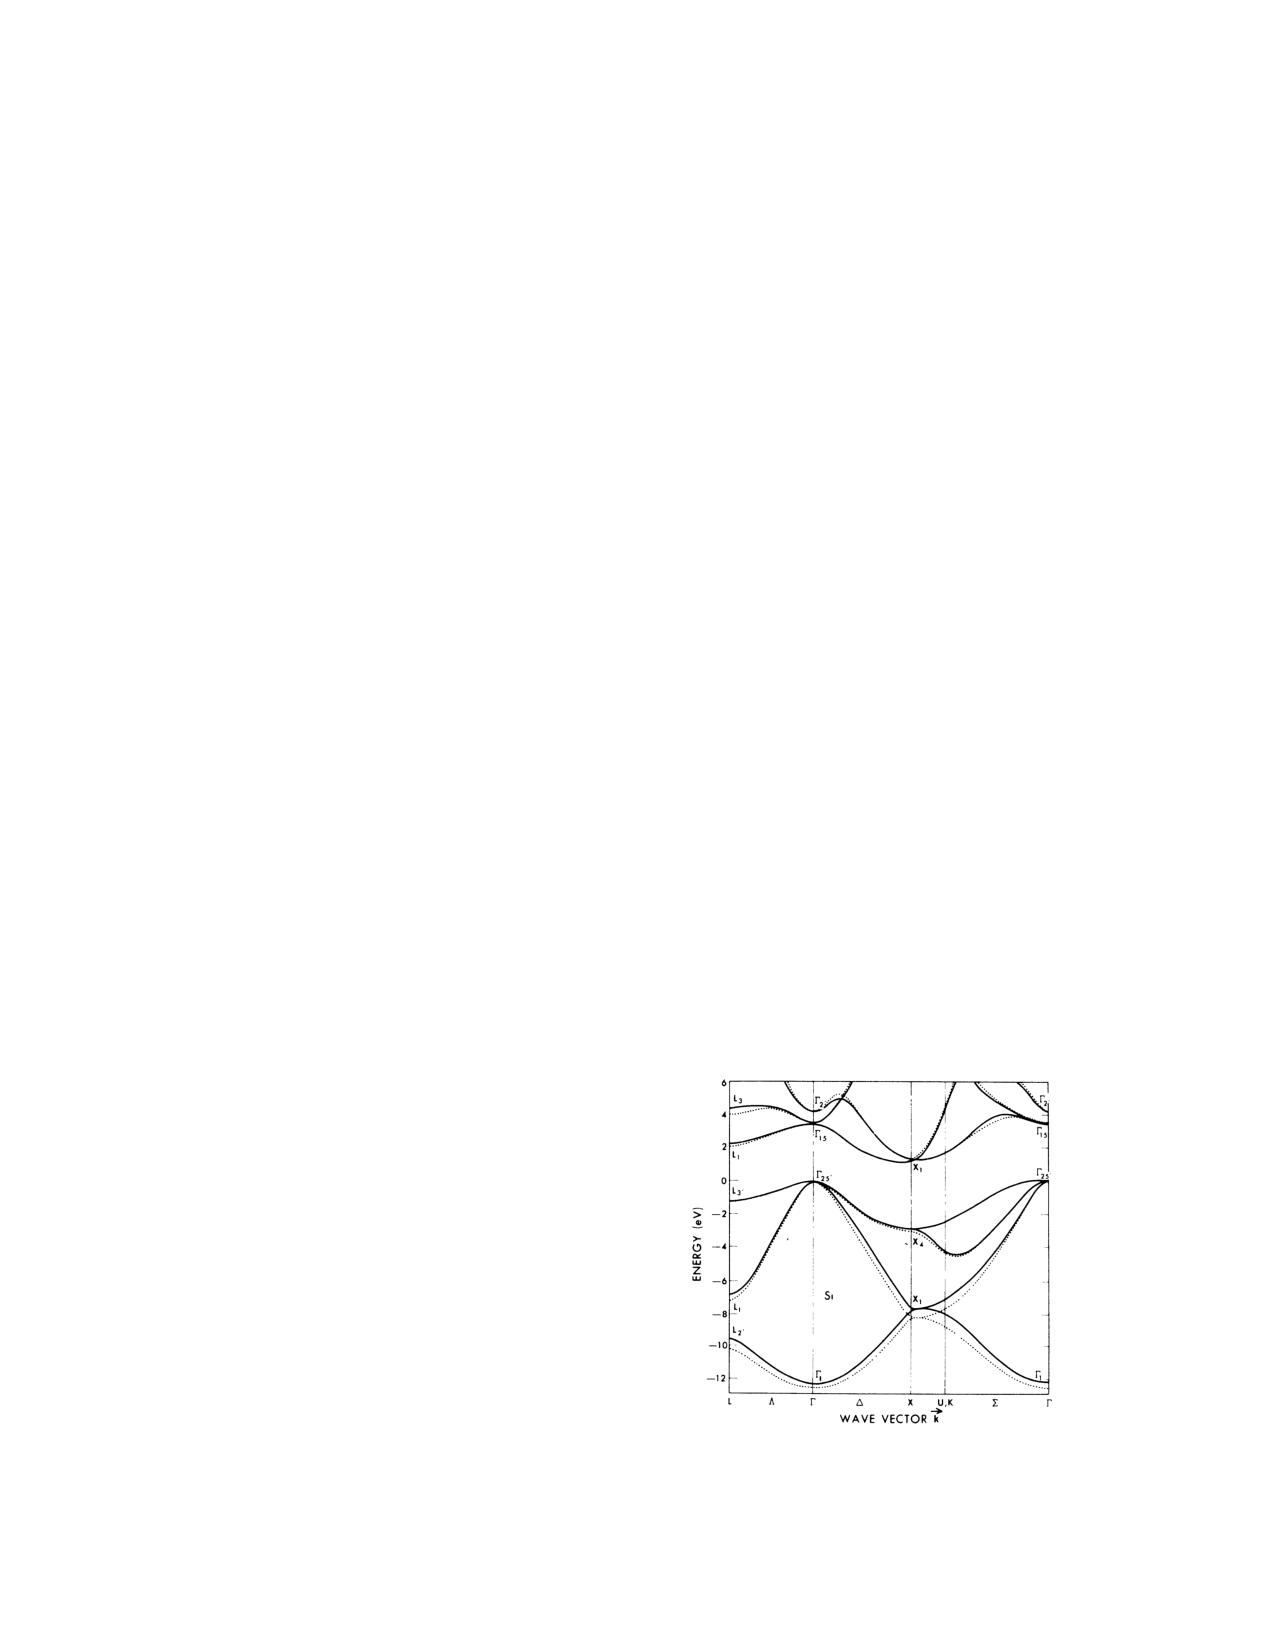
\includegraphics[width = 0.75\columnwidth]{Figures/siliconBandStructure.pdf}
\caption[Silicon band structure]{Figure from \cite{Chelikowsky1974}, showing the band structure of silicon. The top of the valence band is at $\Gamma$, the centre of the Brillouin zone, whilst the minimum of the conduction band is at $X$, towards the edge of the zone.}
\label{fig:siliconband}
\end{figure}

The approach of effective mass theory is to decompose the electron wavefunction into six along these conduction band valleys, giving the equation:

\begin{equation}
\psi(r) = \sum_{\text{i}=1}^6{\alpha_\text{i}\phi_\text{i}(r)F_\text{i}(r)},
\end{equation}

here $\phi_\text{i}(r) = u_\text{i} e^{i \bm{k_\text{i}.r}}$, the Bloch wavefunction such that $u_i(r)$ has the periodicity of the lattice and $\bm{k_\text{i}}=k_0\bm{\text{i}}$ with $k_0$ the momentum value at the valley minimum.
In the electron ground state these valleys are six-fold degenerate, giving the singlet state \cite{Smit2004}:

\begin{equation}
\text{Singlet  } (1sA_{1}) \text{  }
\begin{cases}
\bm{\alpha_g} = \frac{1}{\sqrt{6}}(1, 1, 1, 1, 1, 1)
\end{cases}
\end{equation}

This ground state is the only state with a component of the electron wavefunction at the nucleus and therefore the only one that experiences a hyperfine coupling.
The excited states are as follows:

\begin{equation}
\text{Doublet  } (1sE) \text{  }
\begin{cases}
\bm{\alpha_r} = \frac{1}{\sqrt{12}}(-1, -1, -1, -1, 2, 2)\\
\bm{\alpha_s} = \frac{1}{2}(1, 1, -1, -1, 0, 0)\\
\end{cases}\\
\end{equation}
\begin{equation}
\text{Triplet  } (1sT_2) \text{  }
\begin{cases}
\bm{\alpha_x} = \frac{1}{\sqrt{2}}(1, -1, 0, 0, 0, 0)\\
\bm{\alpha_y} = \frac{1}{\sqrt{2}}(0, 0, 1, -1, 0, 0)\\
\bm{\alpha_z} = \frac{1}{\sqrt{12}}(0, 0, 0, 0, 1, -1)\\
\end{cases}
\end{equation}

When an electric field is applied the symmetry of the valleys is broken leading to the mixing of the various states.
The states interact via the electric dipole moment $e\bm{E.r}$, allowing estimation of the impact via perturbation theory.
The first order perturbation to the singlet state, $\int\bra{\psi_g(r)}e\bm{E.r}\ket{\psi_g(r)}d\bm{r}$ is zero by symmetry \cite{Pica2014}.
The second order perturbation, given by $\sum_{i\neq g}{\int\frac{|\bra{\psi_g(r)}e\bm{E.r}\ket{\psi_g(r)}|^2}{E_g - E_i}d\bm{r}}$ is non-zero however, giving a to the ground state eigenfunction of:

\begin{equation}
\ket{\psi_g(r)} \longrightarrow \ket{\psi_g(r)}\left(1 + \frac{1}{2}\eta_A E^2 \right)+...
\end{equation}

The strength of the hyperfine interaction, $A$, is given by the probability density of the electron wavefunction at the nucleus: $|\ket{\psi_g(r=0)}|^2$.
Thus the change in the hyperfine is given by:

\begin{equation}
\frac{\Delta A}{A} = \frac{|\ket{\psi_g(r=0, E\neq 0)}|^2}{|\ket{\psi_g(r=0, E = 0)}|^2} - 1 = \eta_AE^2 + O(E^4)
\end{equation}

giving a quadratic shift in $E$. $\eta_A$ gives the strength of the shift and is always negative - the mixing with the excited states always reduces the population at the nucleus and thus the hyperfine coupling with it.
\\
In addition to the modulation of the hyperfine coupling there is an effect on the electron g-factor.
The g-factor is determined by the spin-orbit coupling and in general depends on the orientation of the applied magnetic field.
Due to the valley symmetry of the silicon conduction band this anisotropy is normally averaged out but with the application of an electric field this symmetry is broken, changing the electron's orbit and thus its g-factor.
The strength of the effect depends on the axis of electric field.
If this axis is along one of the valley axes ([100] crystal axis) then the effect is maximised.
If it is along the [111] crystal axis then the effect is equal for all valleys, leaving g-factor unchanged.
The g-factor change is given by:

\begin{equation}
\frac{\Delta g_e}{g_e} - 1 = \eta_g(\theta_{BE}, \theta_{BC})E^2
\end{equation}

where $\eta_g$ is the Stark g-factor parameter, $\theta_{BE}$ is the angle between magnetic and electric fields and $\theta_{BC}$ is the angle between the magnetic field and the crystal axis.
\\
Having discussed the theory and background of the Stark shift, I now turn to experimental progress on the subject.

\subsection{Stark Shift Measurement Techniques}

The first approach to measuring the Stark shift would be to take a field sweep.
A field sweep is a standard ESR procedure to determine the magnetic field at which a spin transition occurs for a given microwave frequency.
A standard Hahn echo sequence is performed and the intensity of the echo measured for a given before a new magnetic field is set and the procedure repeated.
At the correct magnetic field for a spin transition an echo will be recorded, with its intensity diminishing to 0 as the magnetic field moves off resonance.
A typical magnetic field sweep for phosphorus doped natural silicon is shown in figure \ref{fig:fieldSweep}.

\begin{figure}
\centering
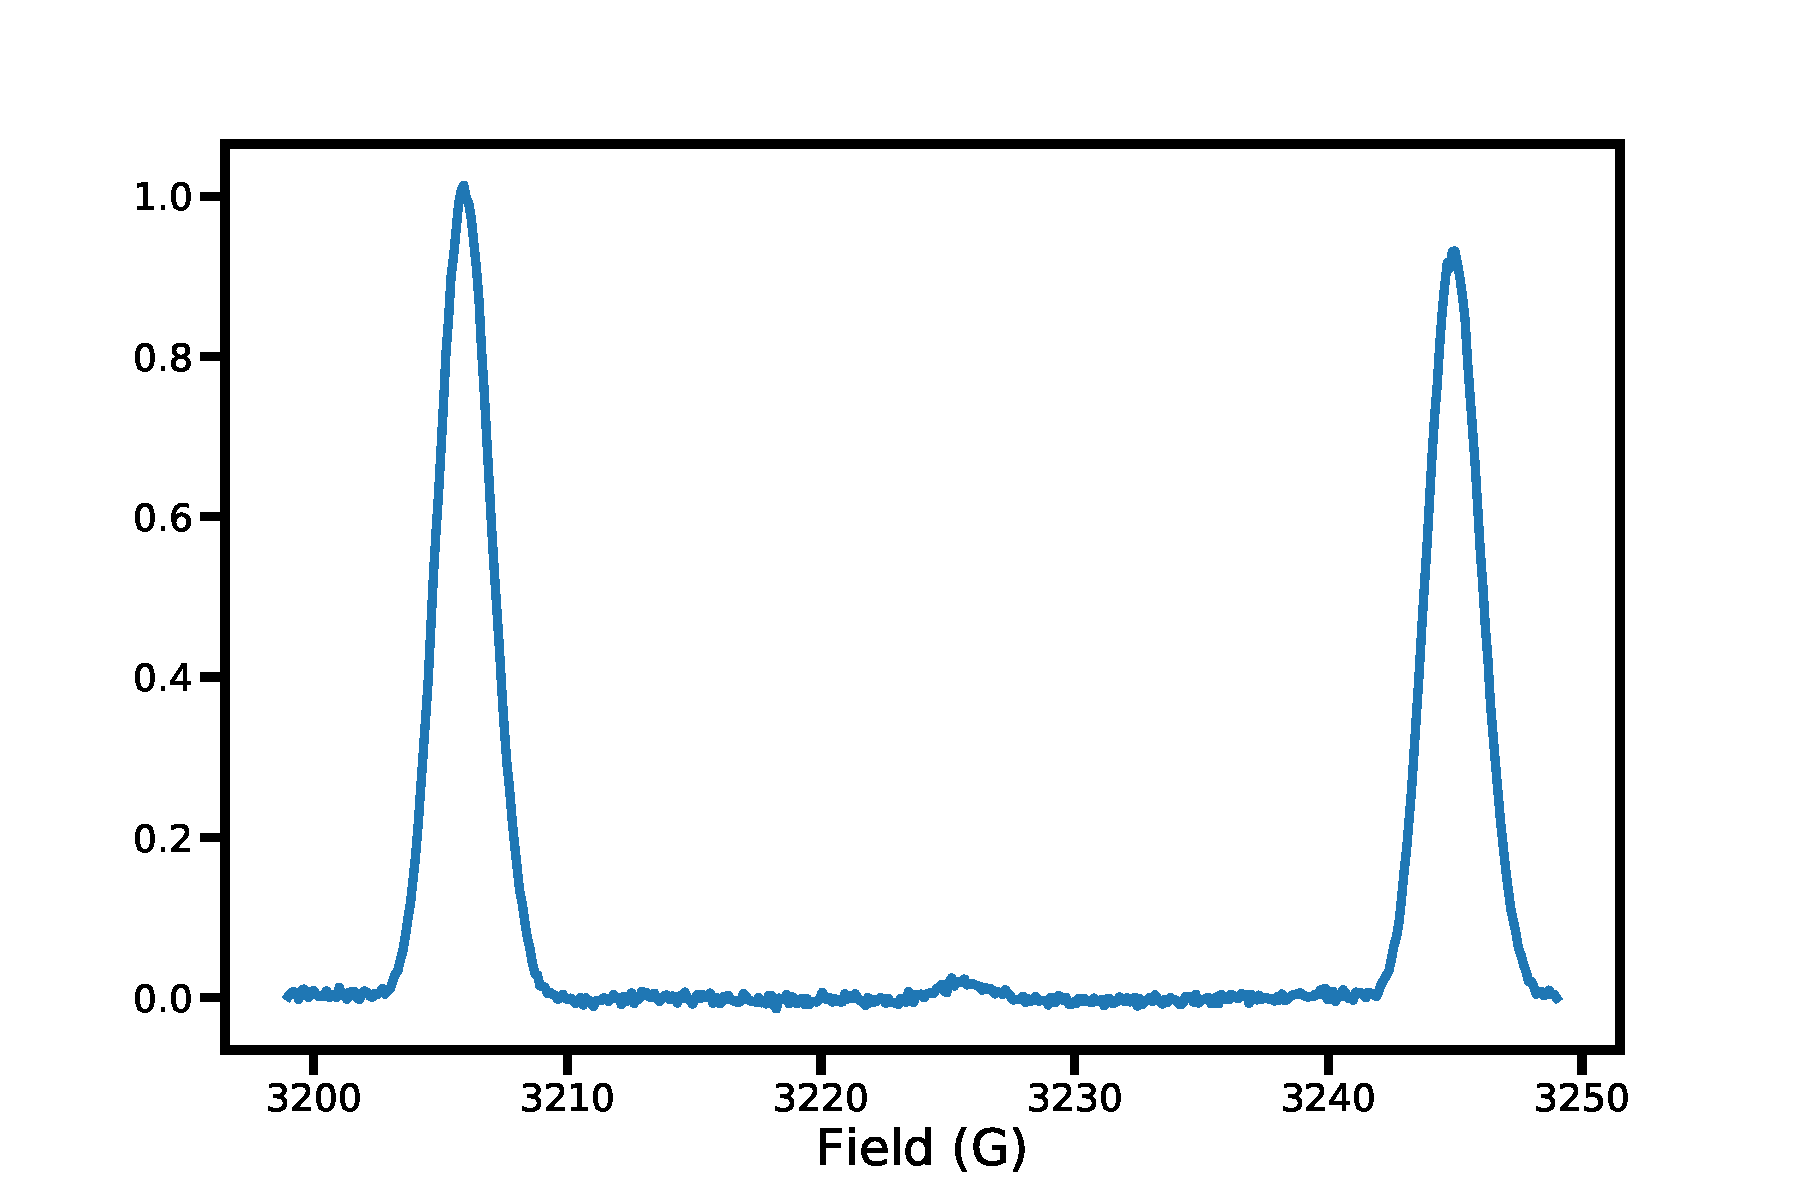
\includegraphics[width=\columnwidth]{Figures/fieldSweep.pdf}
\caption[Phosphorus field sweep]{Graph showing a standard field sweep to locate spin transitions for electrons bound to phosphorus donors in silicon. Hahn echo intensity is recorded for each magnetic field, with the two large peaks corresponding to electrons bound to the two different phosphorus nuclear spins: $\pm \frac{1}{2}$}
\label{fig:fieldSweep}
\end{figure}

This experiment could be undertaken twice, once with electric field on and once with it off.
The Stark shift would produce a change in spin transition frequency which would be observed as a shift in the peaks of the graph.
Unfortunately the Stark shift of the spin transition frequency is typically much smaller than the inhomogeneously broadened linewidth of the spin transition, meaning that no shift is visible \cite{Bradbury2007}.
Instead Bradbury \emph{et al} used a more subtle technique, harnessing the ability of Hahn echo sequence to refocus inhomogeneous broadening.
An electric pulse applied during only one half of a Hahn echo sequence would cause the spins to precess in the magnetic field at different rates when dephasing and rephasing.
This shift can then be detected as a phase shift in the echo intensity from the real to the imaginary channel.
Changing the length of the applied pulse and recording the echo intensity will introduce an oscillation.
The frequency of this oscillation can then be determined using a Fourier transform, thereby giving the Stark shift.
\begin{figure}
\centering
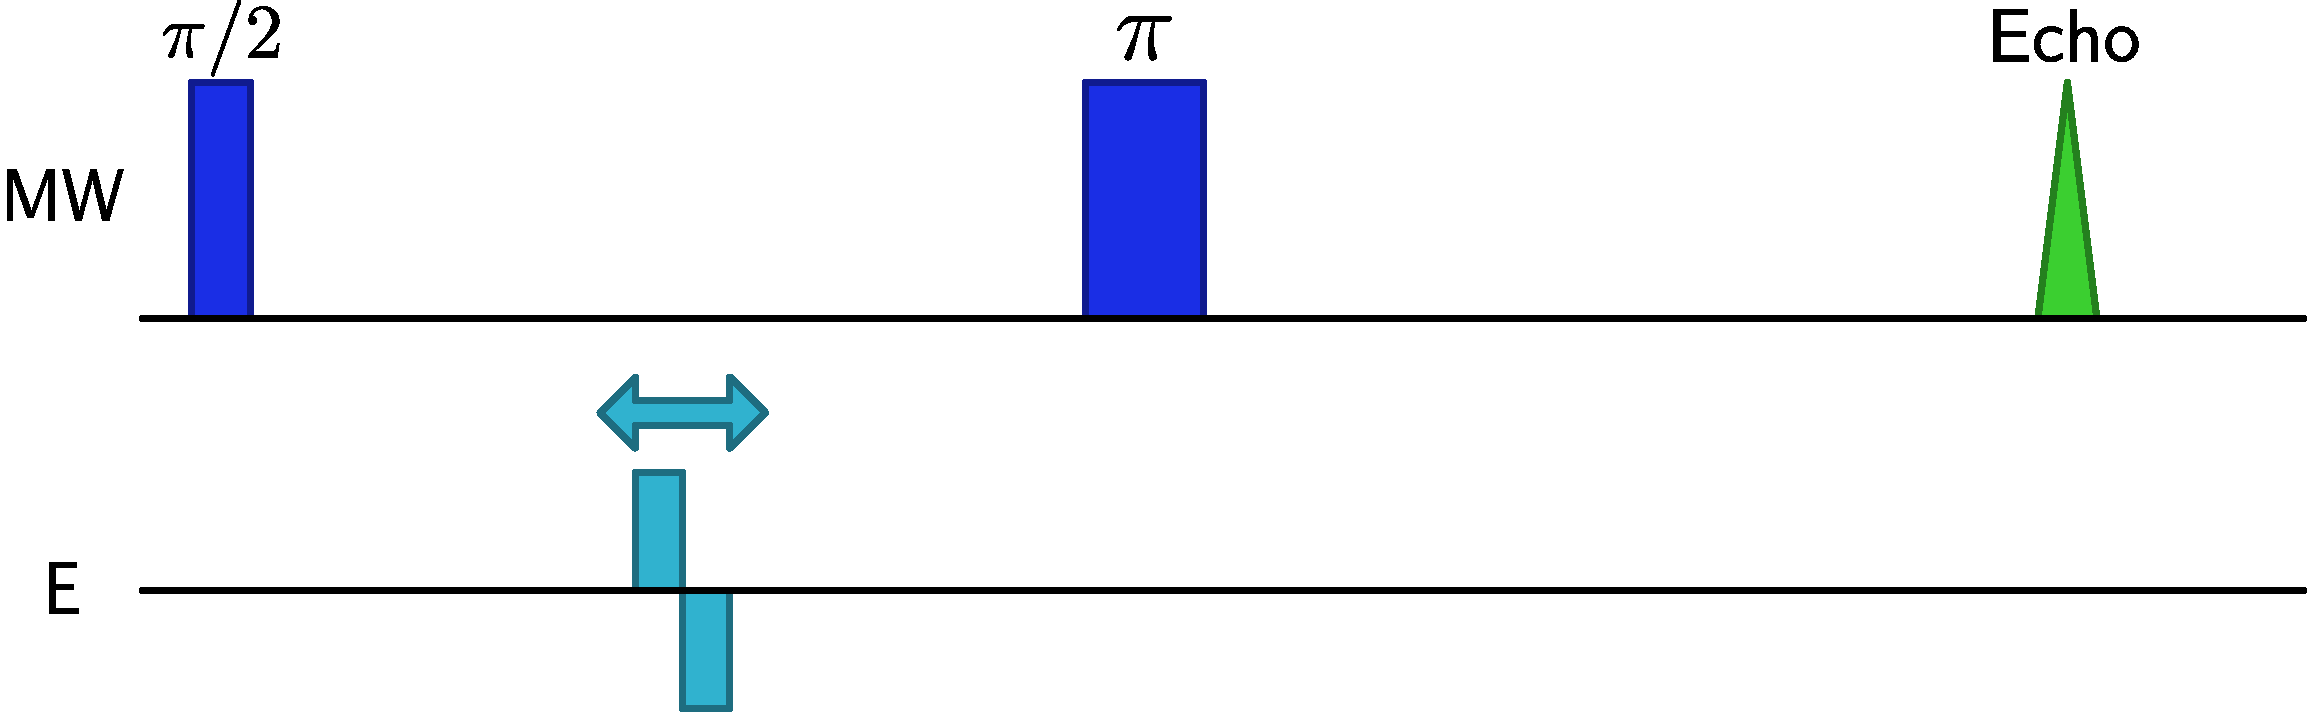
\includegraphics[width=\columnwidth]{Figures/StarkShiftSequenceBasic.pdf}
\caption[Stark shift sequence]{The simplest sequence used to measure a Stark shift on an electron. As the pulse length is increased the electron ensemble acquires a different phase during the first half of the echo compared with the second half, seen as a phase shift in the echo from the real to the imaginary channel.}
\label{fig:starkseq}
\end{figure}
\\
A further effect that must be taken into consideration is the impact of local electric fields.
These are present due to local deformations of the crystal lattice, creating different electric environments at each donor.
In the presence of an external electric field, the total Stark shift of a given donor is given by:

\begin{equation}
\left (E_{\text{local}} + E_{\text{ext}} \right)^2 = E_{\text{local}}^2 + E_{\text{ext}}^2 + E_{\text{local}}E_{\text{ext}}
\end{equation}

The inhomogeneity of the local fields would usually provide a simple offset in the phase shift, but the term that is linear in both $E_{\text{local}}$ and $E_{\text{ext}}$ causes the inhomogeneity to get larger as the applied field gets larger.
This would result in a rapid decay of the echo signal, but can be avoided by applying a bipolar electric field pulse (i.e. half negative, half positive), a technique implemented by Bradbury \emph{et al} when measuring the Stark shift of antimony donors in silicon \cite{Bradbury2007}.
This cancels the linear term but has no impact on the quadratic term.
This sequence can be seen in figure \ref{fig:starkseq}.

\subsection{Stark Shift Experimental Results}

Measurements of the Stark shift on all group V donors in silicon were undertaken by Wolfowicz \emph{et al} \cite{Wolfowicz2014,Pica2014}.
The experiment was performed using bulk doped samples of silicon, placed between copper plates.
The copper plates were connected to an operational amplifier with an amplification factor of 126.
Pulses were generated using an arbitrary wave generator.
Results of their measurements are shown in figure \ref{fig:garyStarkResults}.

\begin{figure}
\centering
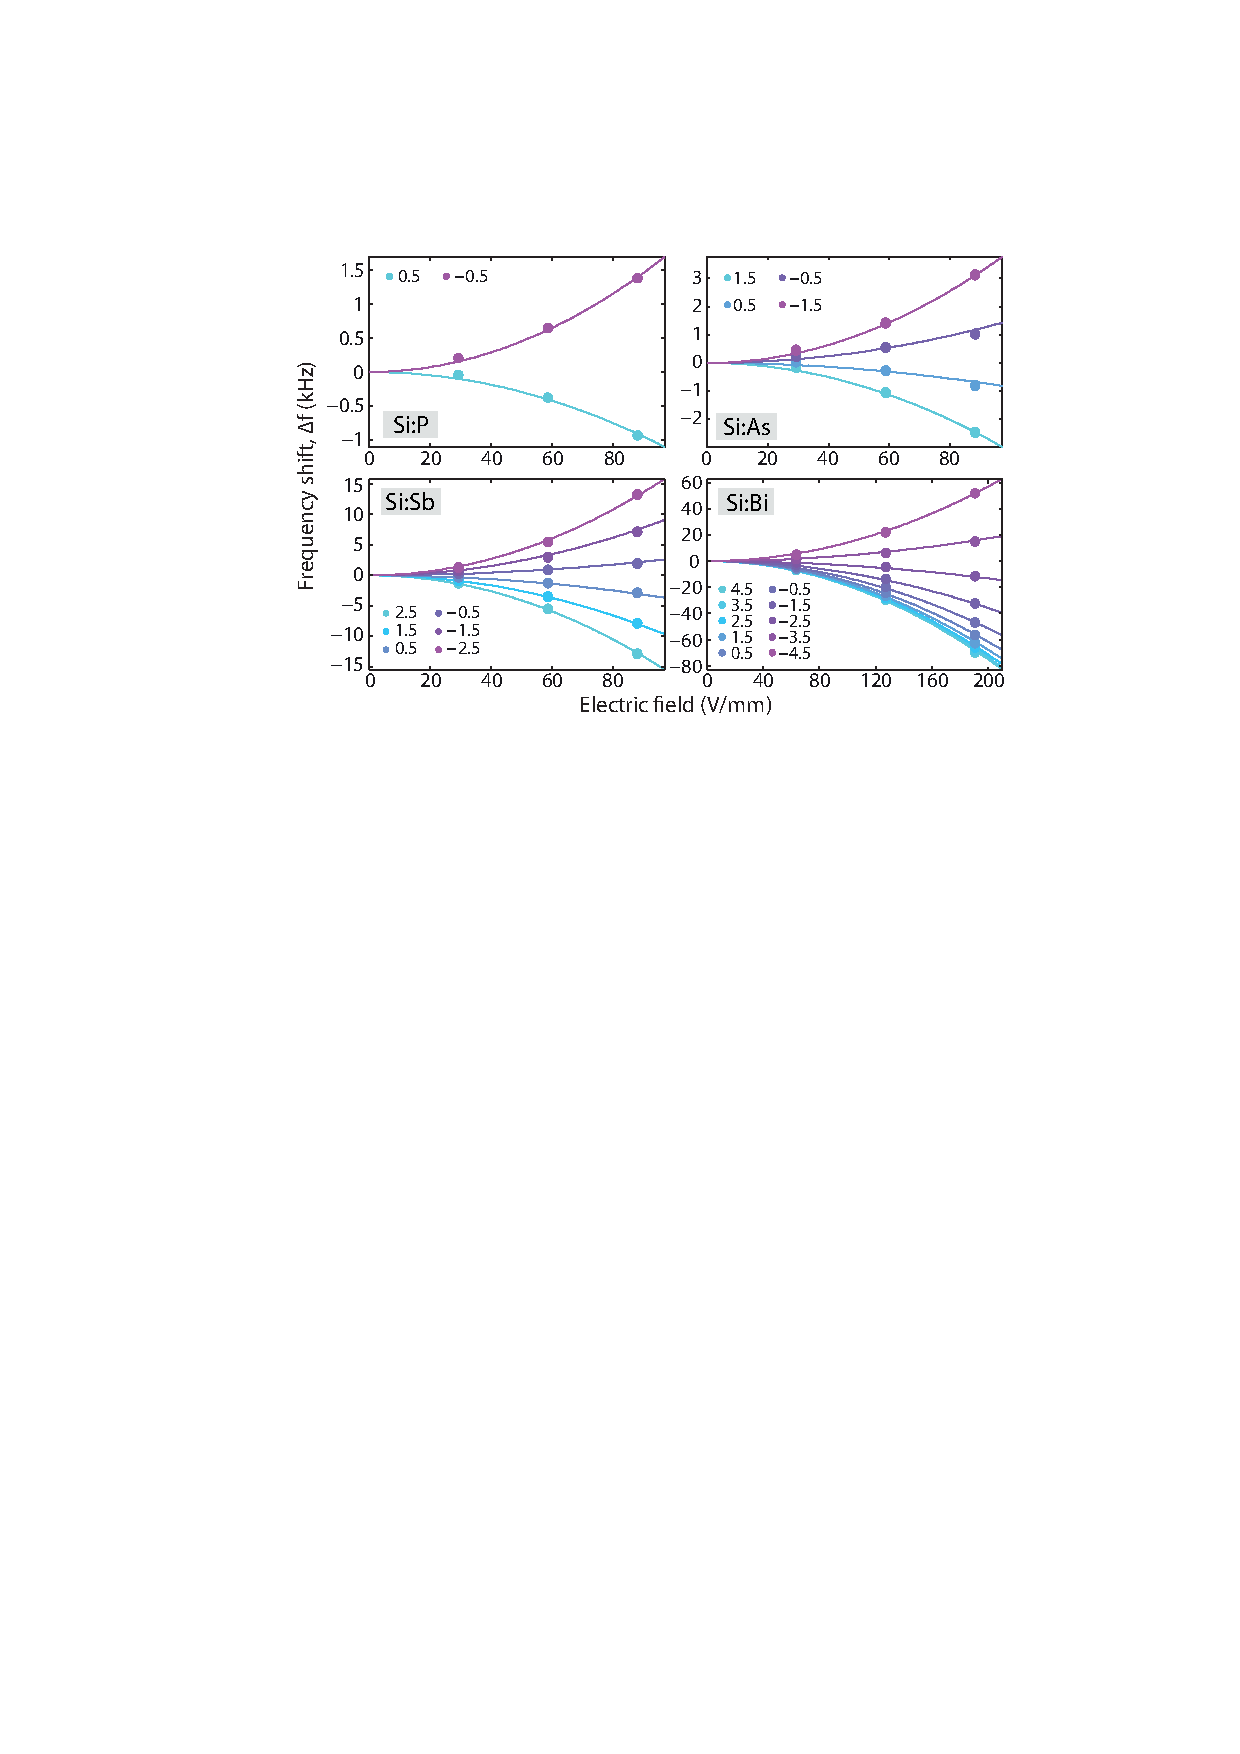
\includegraphics[width=0.75\columnwidth]{Figures/starkShiftResultsGary.pdf}
\caption[Wolfowicz \emph{et al} Stark measurements]{These figures demonstrate the frequency shift in the spin transition as a result of the Stark shift, as measured by Wolfowicz \emph{et al} \cite{Wolfowicz2014}. Notable is the increased rate for higher nuclear spin numbers - this is due to the shift being proportional to the hyperfine coupling, which is in turn proportional to nuclear spin.}
\label{fig:garyStarkResults}
\end{figure}

These measurements determined the following Stark shift parameter for $\eta_A$, with $\eta_g$ being smaller than the measurement sensitivity:

\begin{center}
\begin{tabular}{||c || c | c | c | c||}
\hline
& $^{31}$P & $^{75}$As & $^{121}$Sb & $^{209}$Bi \\
\hline
$\eta_A (\times 10^{-3} \mu m^2 / V^2)$ & $-2.5\pm 0.5$ & $-1.2 \pm 0.1$ & $-3.5 \pm 0.05$ & $-0.26\pm0.05$\\
\hline
\end{tabular}
\end{center}

Wolfowicz \emph{et al} also performed experiments to test conditional control of the spins using Stark shifts.
The aim of such an experiment is to shift the transition frequency of the selected spin by several times its linewidth.
This was not possible for the electron due to its broad linewidth even in purified silicon.
Instead the experiment was performed on the nuclear transition, which has a much narrower linewidth due to its smaller dipole moment.
By applying an electric field at the same time as nuclear spin $\pi$ pulse, Wolfowicz \emph{et al}, the process is measured as an identity with fidelity 93.3$\pm2.6\%$.
This indicates that it is possible to control the application of pulses to nuclear spin qubits using electric fields as required by the Kane proposal.
What is less clear is whether these spin qubits will be sufficiently resistant to any stray electric fields in a scalable quantum computing architecture.

\subsection{The Nuclear Spin Bath in Natural Silicon}

% \subsection{Introduction}

The presence of $^{29}$Si nuclei in natural silicon has been discussed earlier as one of the chief factors impacting qubit coherence times in that medium.
Inhomogeneous hyperfine interactions between these spins and addressed electron spins leads to spectral diffusion and reductions in coherence times for qubits in natural silicon.
Although most proposals for silicon donor qubit architectures have involved purified silicon to avoid these issues, a proposal has been put forward to use these impurity spins as a quantum register with applications for error correction \cite{Wolfowicz2016a}.
From the perspective of the O'Gormann proposal, these spins could present a potential quantum register for data qubits, providing storage for their spin states during long computations.
In order to control the interaction between data qubits and the $^{29}$Si nuclear spins the Stark shift will be necessary to control the transition frequency of a given spin relative to an external control pulse.
Attempting to characterise the Stark shift of the hyperfine coupling between the electron and the $^{29}$Si nuclei will be a goal of this report.

% !TEX root = ../Thesis.tex
\chapter{Experimental Methods}


\section{Equipment}
\subsection{Cryogenic and Microwave Instrumentation}

The experiments in this report were performed in an Oxford Instruments CF935 Helium flow cryostat.
A dewar of Helium is connected to this cryostat via a vacuum-insulated transfer arm and kept at approximately 500mBar overpressure, to facilitate cooling without an external pump.
Flow into the cryostat is controlled via a valve for coarse temperature control and a heater at the bottom of the cryostat is used along with a PID controller for fine-grained temperature control.
A Bruker electromagnet provides a static field of up to 1.5 Tesla for ESR measurements.
\\
For ESR measurements a Bruker E500 X-Band spectrometer is used, with the pulses generated amplified via a travelling wave tube amplifier.
The time resolution on this spectrometer is 4~ns.
Pulses generated enter a Bruker resonator, placed in the cryostat, which has a split ring cavity at the base with the sample at the centre.
Microwave pulses entering this cavity generate an oscillating magnetic field at the sample for electron spin control.
The resonant frequency of this cavity is fixed at a given temperature but some tuning of its q-factor is possible.
This is necessary to ensure that the bandwidth of the cavity is broad enough to admit all control pulses (bandwidth of a pulse is approximates 1/(pulse length)) and to ensure an appropriate cavity ring-down time.
The spectrometer also provides an RF output for nuclear spin control, this is amplified separately and then input into the same resonator.
\\
The electron spin signal is detected through the same channel: the oscillating magnetic field generated by the precessing electrons is demodulated with the same frequency as the control pulse.
When the control signal is on resonance this provides two DC signals, one from the in phase (real) component of the demodulation and one from the out of phase (imaginary).This signal decays according to the $T_2^*$ time to provide the characteristic spin echo.
This is captured using Bruker's Xepr software, which can integrate under the echo to record changes in intensity.

\subsection{Laser}

The main laser used in this report is a Toptica DL Pro - a tunable diode laser with a range from approximately 1060~nm to 1080~nm.
This laser can be tuned in two ways: the first is a coarse tuning which is achieved by manually changing the cavity size via a control knob.
The second is a fine tuning achieved electronically, this is useful for extremely precise wavelength tuning such as is necessary for bound-exciton experiments or spectroscopy but is not used in this report.
The laser has a linewidth of 100~kHz and an output power of up to 130mW.

\section{Pulse Sequences}


\subsection{ESR Pulse Sequences}

All experiments in this report are performed using various ESR pulse sequences.
The simplest of these is the Hahn echo sequence, described above and depicted in figure \ref{fig:HahnEcho}.
Several steps are involved to optimise an ESR experiment, the first of which is determining the magnetic field required to excite a spin transition.
The microwave frequency is fixed by the cavity so magnetic field must be changed - this is done via a field sweep as described above, the results of which are shown in \ref{fig:fieldSweep}.
Another critical factor is determining the required length of a $\pi$ pulse at a chosen power.
This is achieved via a \emph{Rabi} sequence, this involves a regular Hahn echo sequence with an additional pulse before the first $\pi/2$ pulse.
The length of this pulse is changed and the echo intensity recorded.
As this length changes the echo intensity will oscillate, with the frequency of the oscillation giving the correct $\pi$ pulse length.
This sequence is shown in figure \ref{fig:Rabi}.

\begin{figure}
\centering
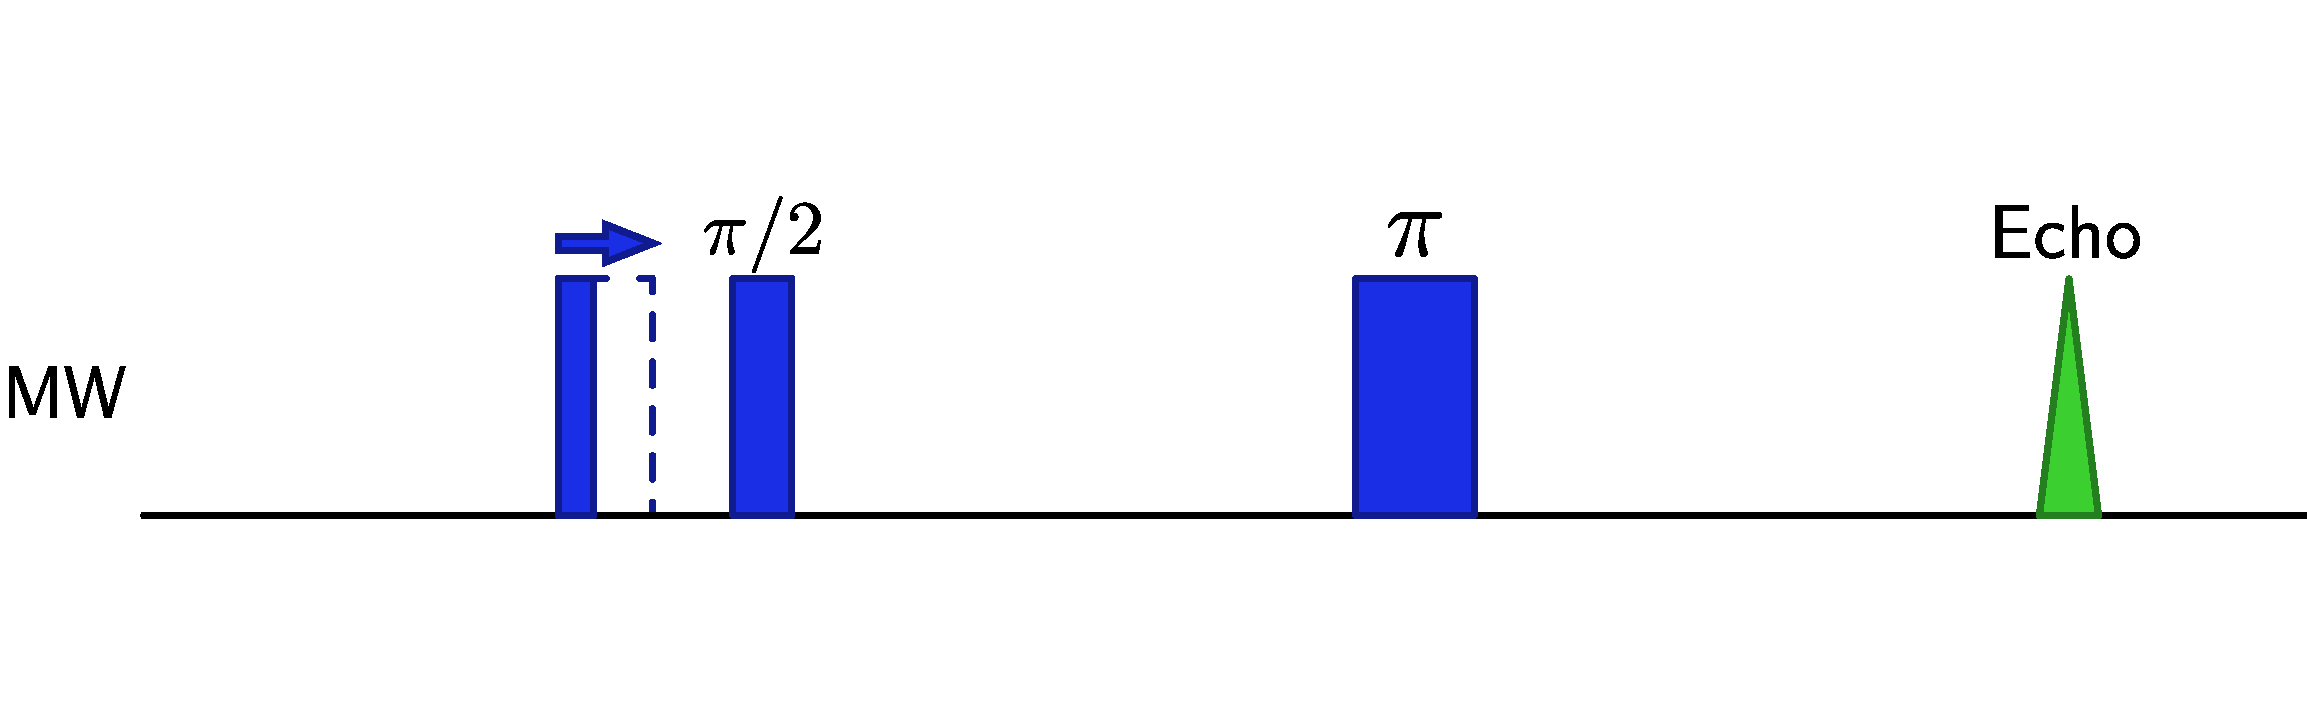
\includegraphics[width = \columnwidth]{Figures/Rabi.pdf}
\caption[Rabi Sequence]{The Rabi pulse sequence, used to determine ideal $\pi$ pulse length at a given power. Creates an oscillation in echo signal as initial pulse length is changed with the rate of oscillation giving the ideal pulse length}
\label{fig:Rabi}
\end{figure}

Two vital pulse sequences are those that determine the $T_1$ and $T_2$ times of a given sample and under given conditions.
The pulse sequence to determine $T_1$ is the \emph{inversion recovery} sequence.
This consists of a Hahn echo sequence preceded by a $\pi$ pulse, which inverts the echo signal.
The time between the initial $\pi$ pulse and the Hahn echo sequence is increase, resulting in an inverted exponential decay as the echo recovers from fully inverted to fully positive.
This occurs as the polarisation reverts to thermal equilibrium between the initial $\pi$ pulse and the Hahn echo sequence, with the time constant of the decay giving $T_1$.
\\
To determine $T_2$ the standard experiment is a regular Hahn echo sequence with $\tau$, the time between $\pi/2$ and $\pi$, and between $\pi$ and echo increased.
This measures the rate at which spin decoherence occurs - as the spins precess for longer in the magnetic field they gradually acquire irreversible phase differences.
As these build up the echo signal decreases exponentially, with the time constant of this decay giving $T_2$.

\begin{figure}
\centering
\begin{subfigure}[t]{\columnwidth}
\centering
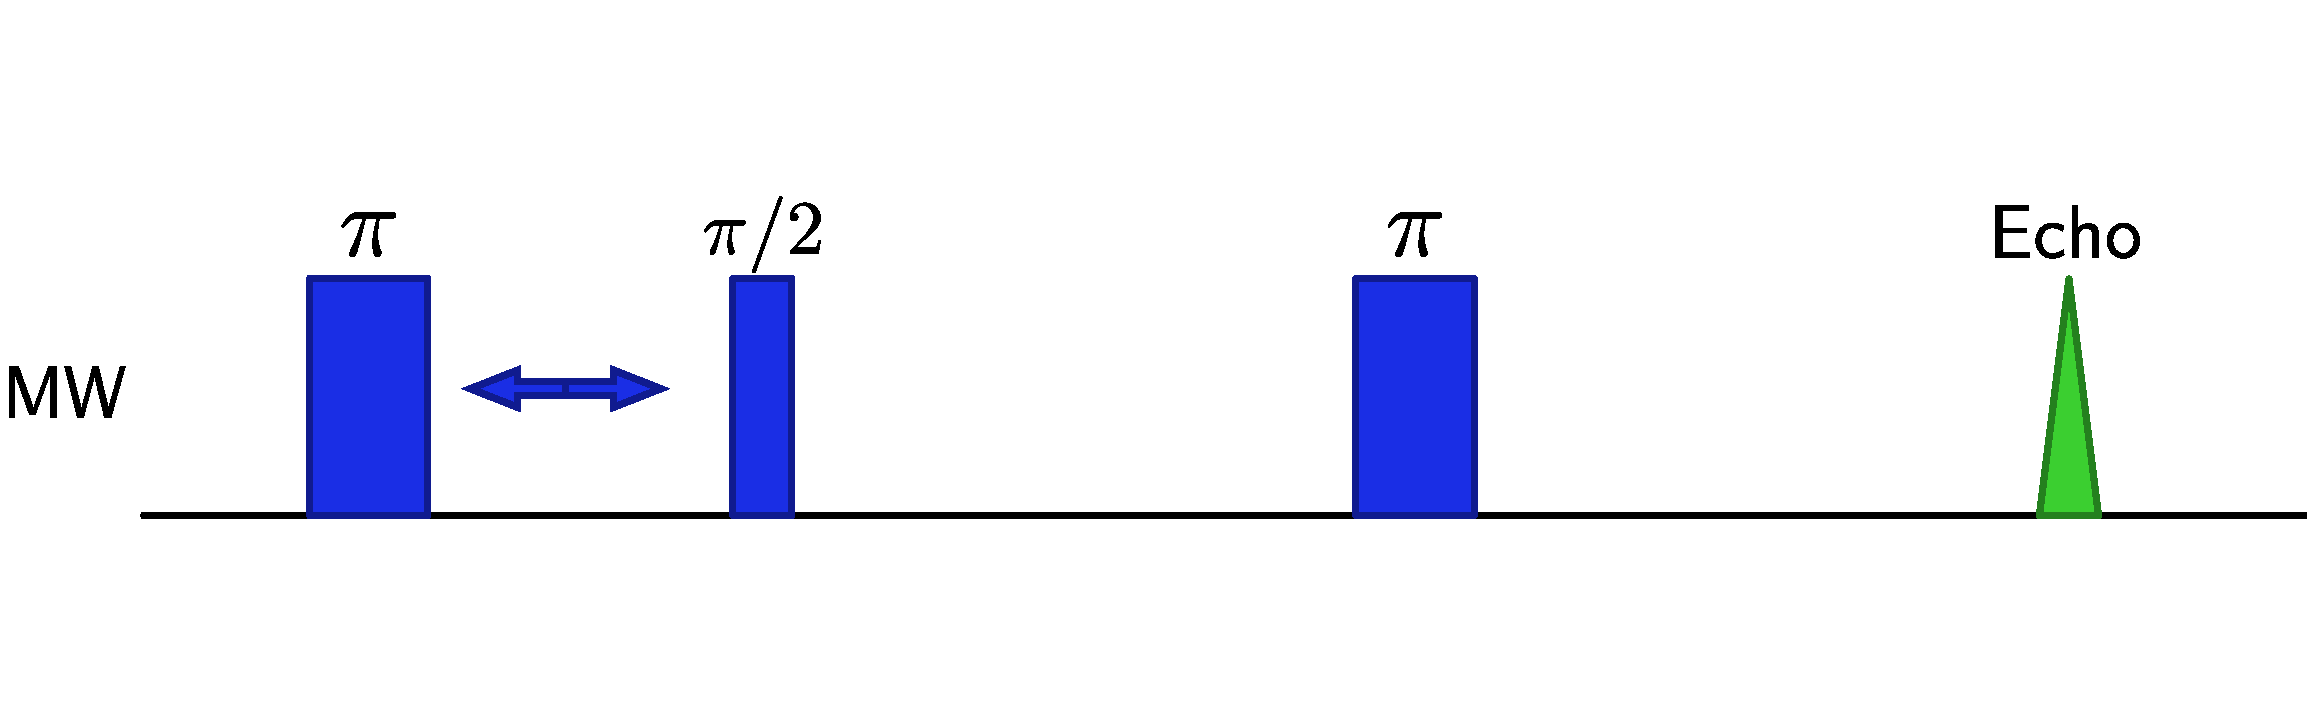
\includegraphics[width=\columnwidth]{Figures/inversionRecovery.pdf}{a}
\end{subfigure}
\begin{subfigure}[t]{\columnwidth}
\centering
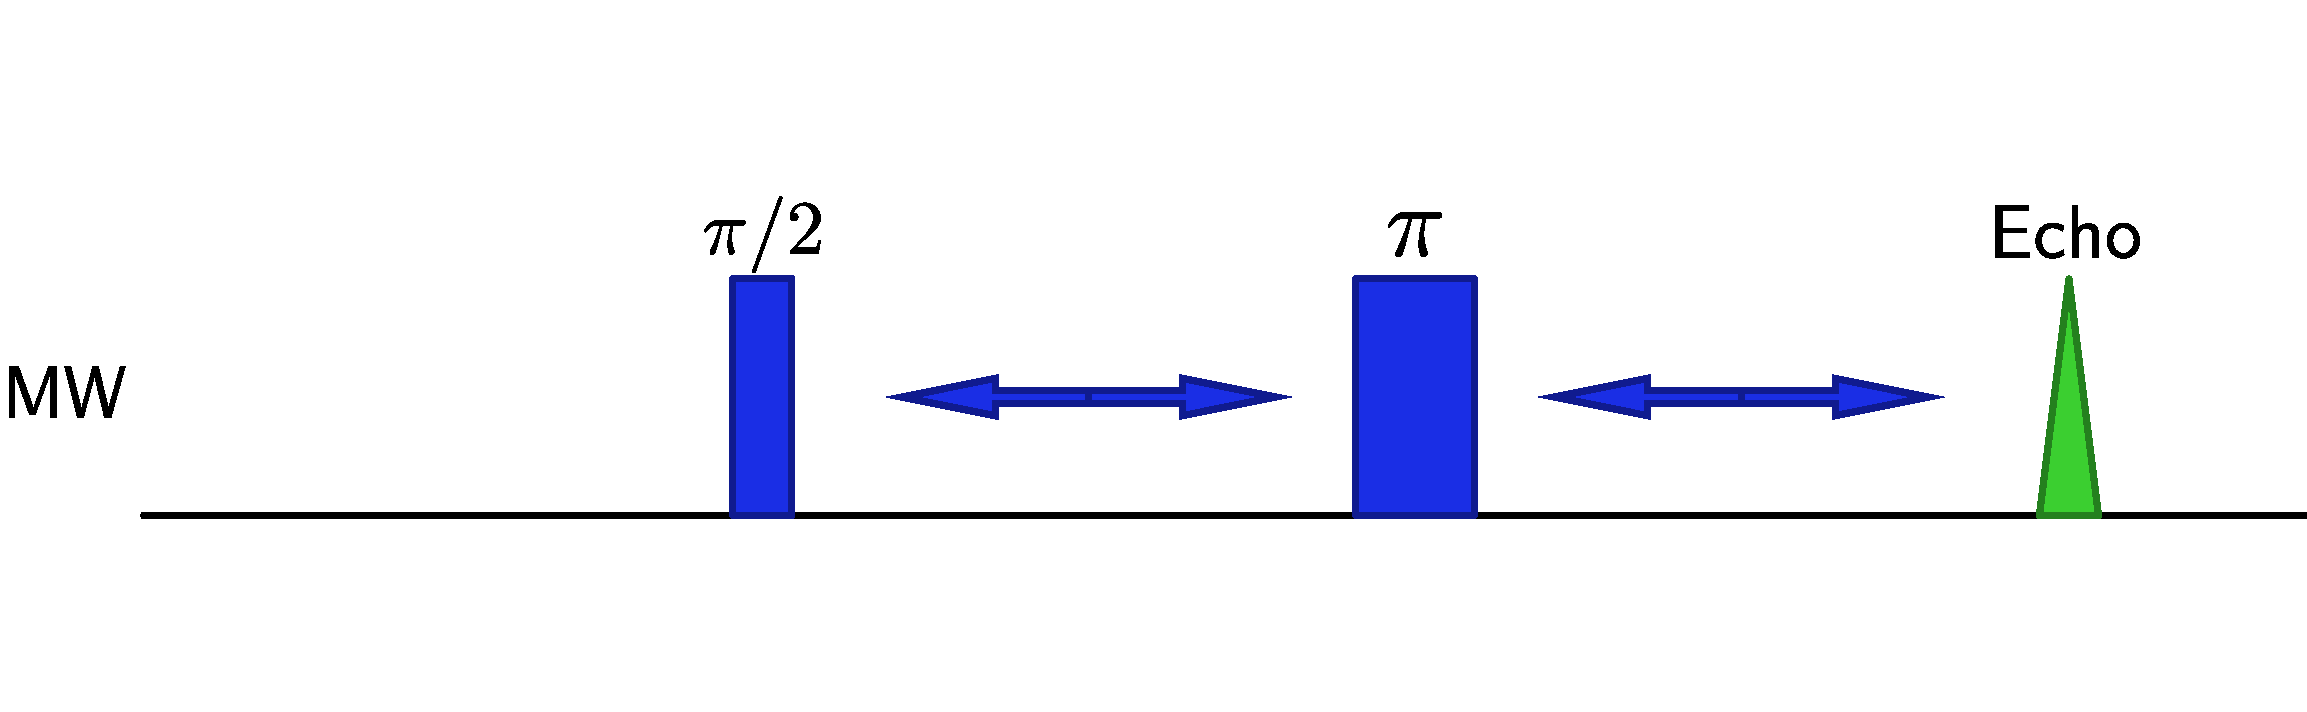
\includegraphics[width=\columnwidth]{Figures/t2.pdf}{b}
\end{subfigure}
\caption[Inversion recovery and $T_2$ pulse sequences]{Cartoons depicting pulse sequences for measurement of $T_1$, a, and $T_2$, b. Inversion recovery measures $T_1$ by inverting the typical spin polarisation with an initial $\pi$ pulse and increasing the time between this and a Hahn echo sequence. As the time is increased the polarisation has longer to relax to thermal equilibrium, meaning it slowly recovers from fully negative to fully positive in an inverted exponential decay whose time constant is $T_1$. $T_2$ is measured using b, which increases the $\tau$ value of the Hahn echo sequence, meaning spins precess in the magnetic field for longer. As they do so they acquire irreversible phase differences leading to the decay of the Hahn echo signal with an exponential decay constant $T_2$.}
\label{fig:t1t2}
\end{figure}

\subsubsection{Dynamical Decoupling}

A set of pulse sequences all of which attempt to increase coherence times are known collectively as \emph{dynamical decoupling} sequences.
At their simplest these add a number of extra $\pi$ pulses between the initial $\pi/2$ pulse and the echo.
Although a full theoretical treatment is complex and well beyond the scope of this work, a physical intuition is relatively easily gained.
These pulses reduce the impact of time varying magnetic fields, by effectively narrowing the bandwidth of magnetic noise frequencies that the donor spin is sensitive to \cite{Wang2009}.
This is done by shortening the time that the electrons precess before they are flipped by a $\pi$ pulse.
Doing this means that slower changing magnetic fields have less of an impact on decoherence - between each reversal of phase acquisition there will have been little field change, meaning that any phase acquired is reversed.
\\
Although more complex sequences exist than simple repetition of $\pi$ pulses, such as Uhrig Dynamical Decoupling \cite{Uhrig2008}, the only one used in this report is the CPMG pulse, a cartoon of which is shown in figure \ref{fig:CPMGpulse}.
Important to note is that the $\pi$ pulses are applied along an orthogonal rotation axis to the $\pi/2$ pulse as this renders the sequence less susceptible to pulse errors \cite{Carr1954,Meiboom1958}.


\begin{figure}
\centering
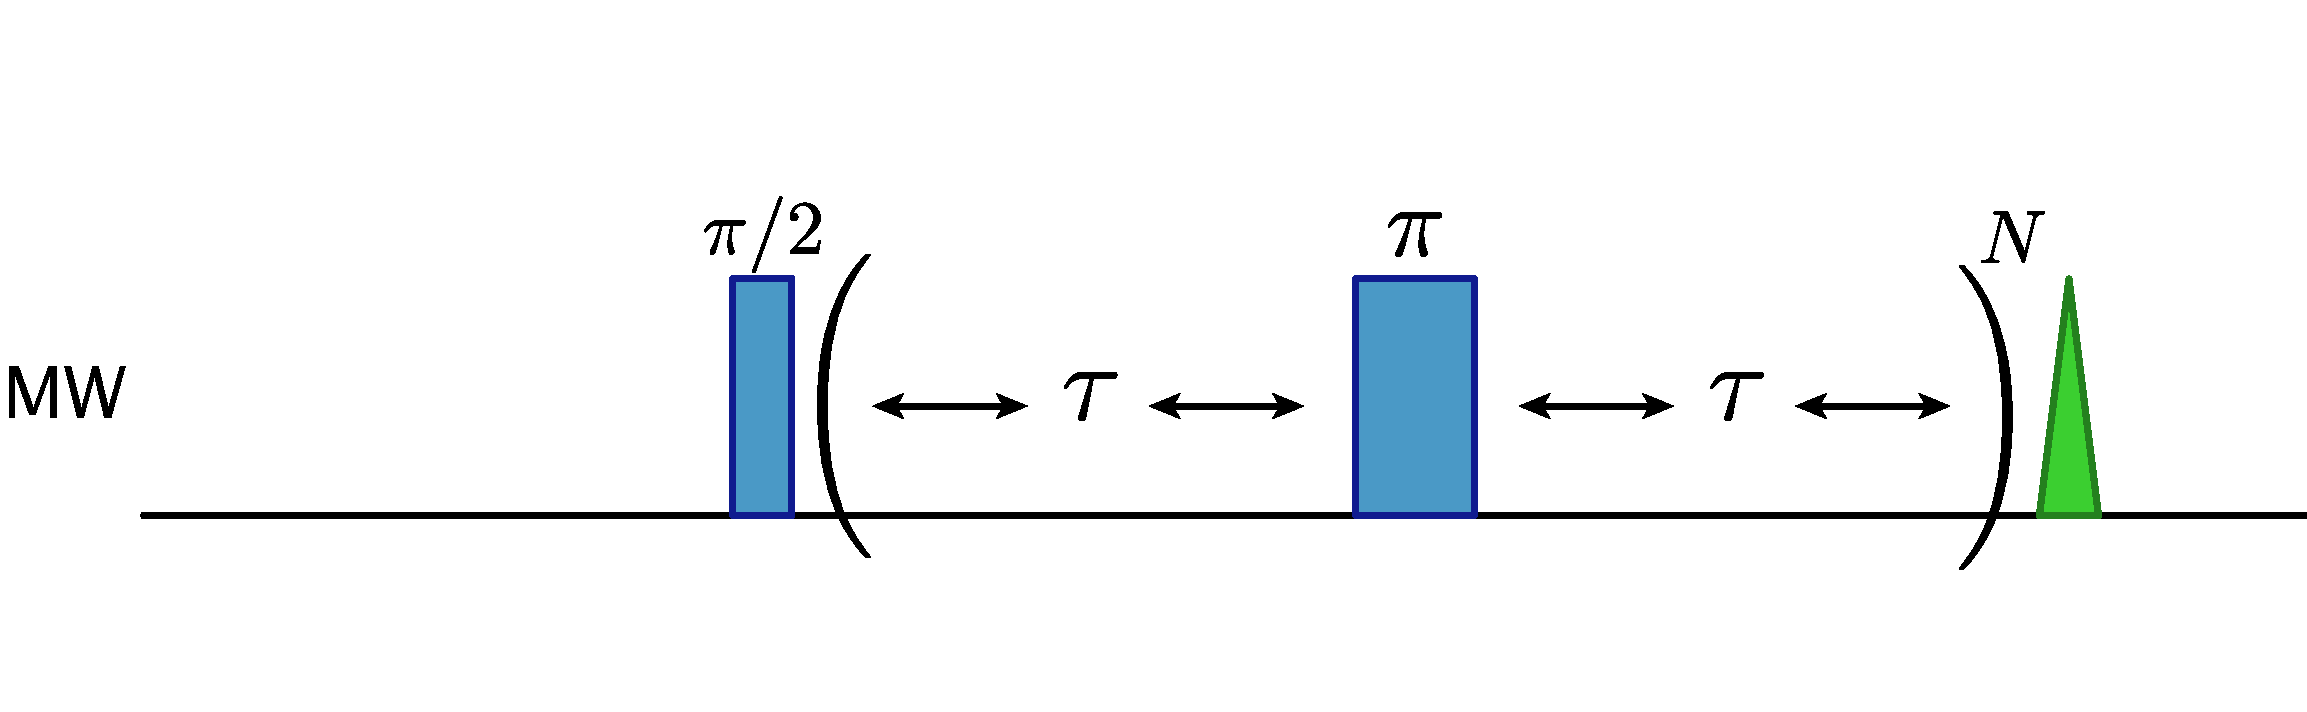
\includegraphics[width=\columnwidth]{Figures/CPMG.pdf}
\caption[CPMG pulse sequence]{The CPMG dynamical decoupling sequence, which uses successive $\pi$ pulses to reduce the bandwidth of noise that the donor spins are exposed to, thereby increasing effective decoherence time.}
\label{fig:CPMGpulse}
\end{figure}

\subsection{Nuclear Spin Pulse Sequences}

Measurements of nuclear spins can be undertaken directly, as is performed in NMR studies, but their significantly weaker signal relative to the electron (due to their much smaller polarisation) makes this technique troublesome.
The process undertaken when a coupled electron-nucleus system exists is based around ENDOR (Electron Nuclear Double Resonance) sequences.
These sequences are based around transferring the electron polarisation to the nuclear spin, thereby magnifying the signal to the same level as the electron.
The first and simplest of these is the Davies ENDOR sequence, shown in figure \ref{fig:DaviesENDOR}.
This sequence first inverts the electron polarisation on one nuclear spin transition before using a nuclear $\pi$ pulse to transfer it to the opposite nuclear spin transition.
This results in an equal polarisation between the two electron spin states so the echo intensity is reduced to 0 in the case of a perfect $\pi$ pulse.



\begin{figure}
\centering
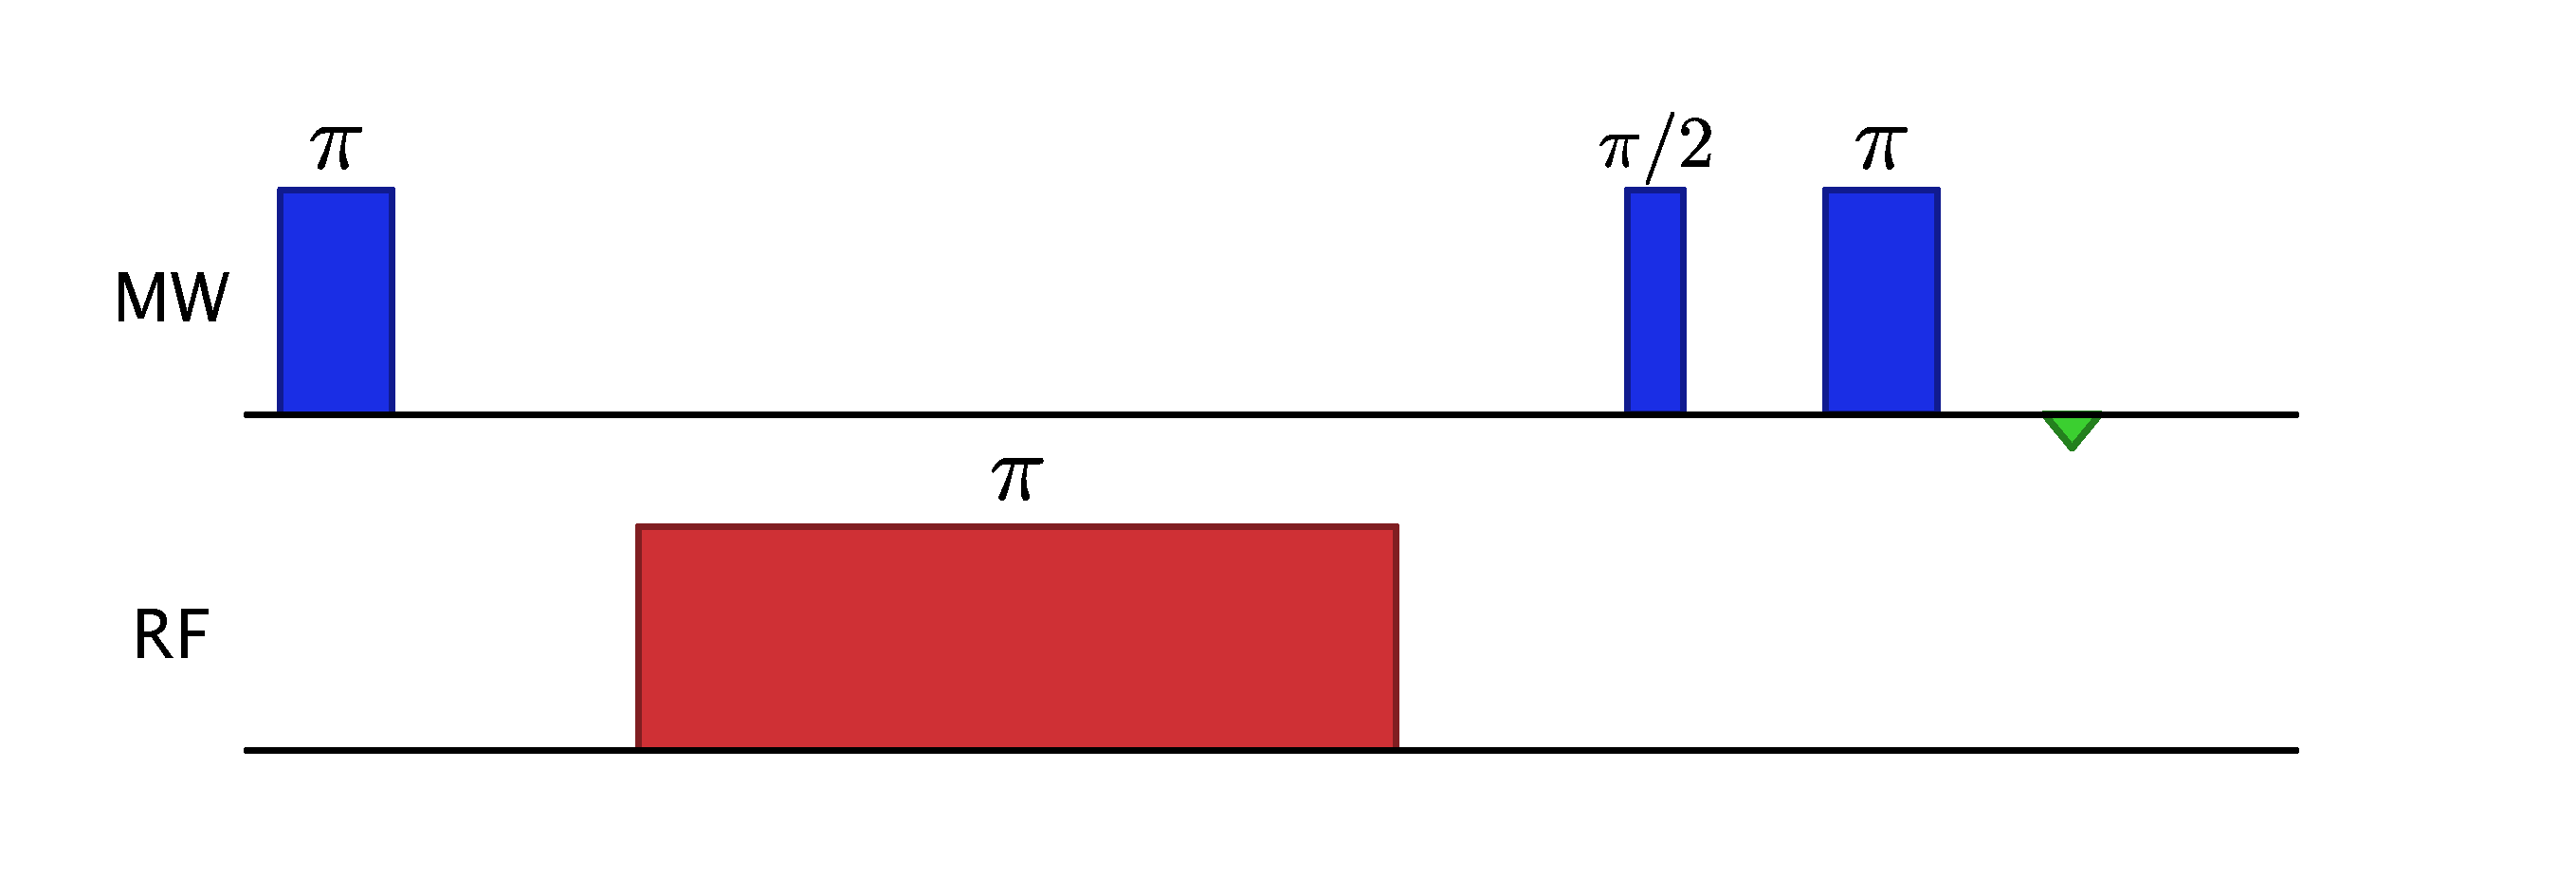
\includegraphics[width=\columnwidth]{Figures/daviesENDOR.pdf}
\caption[Davies ENDOR sequence]{This is the simplest sequence with which to identify nuclear spin transitions. The electron spin polarisation is inverted before nuclear $\pi$ pulse transfers it to the opposite nuclear spin state. This renders the population between the two electron spin states equal, reducing the echo intensity to 0 in the case of a perfect nuclear $\pi$ pulse.}
\label{fig:DaviesENDOR}
\end{figure}

One potential problem is the long nuclear $T_1$ time, which can prevent the usual approach to resetting the sample between experiments of waiting for all spins to relax to thermal equilibrium.
Continued experiment without relaxation rapidly reduces the signal as the spin transition is saturated.
To avoid this a second $\pi$ pulse (Tidy pulse) is usually added after the echo detection to reset the nuclear spin polarisation to its thermal equilibrium value \cite{Morton2008a}.
This sequence can be used to find nuclear transitions by sweeping the RF frequency of the nuclear $\pi$ pulse and also to measure the nuclear Rabi frequency by sweeping the pulse length when a transition has been located.
\\
Another useful nuclear sequence is the nuclear echo, which can be used to measure the $T_2^*$ time of the nuclear spins and a variant is used in this report as a means of measuring the Stark shift.
This uses a sequence of two nuclear $\pi$ pulses with a nuclear $\pi/2$ pulse in between.
The time between the initial $\pi$ and $\pi/2$ pulses is kept constant, whilst the time to the final $\pi$ pulse is swept.
This produces a nuclear signal that increases and decays according to the nuclear $T_2^*$ time, with its maximum signal when the pulses are equidistant in time.
This is shown in figure \ref{fig:nuclearecho}.

\begin{figure}
\centering
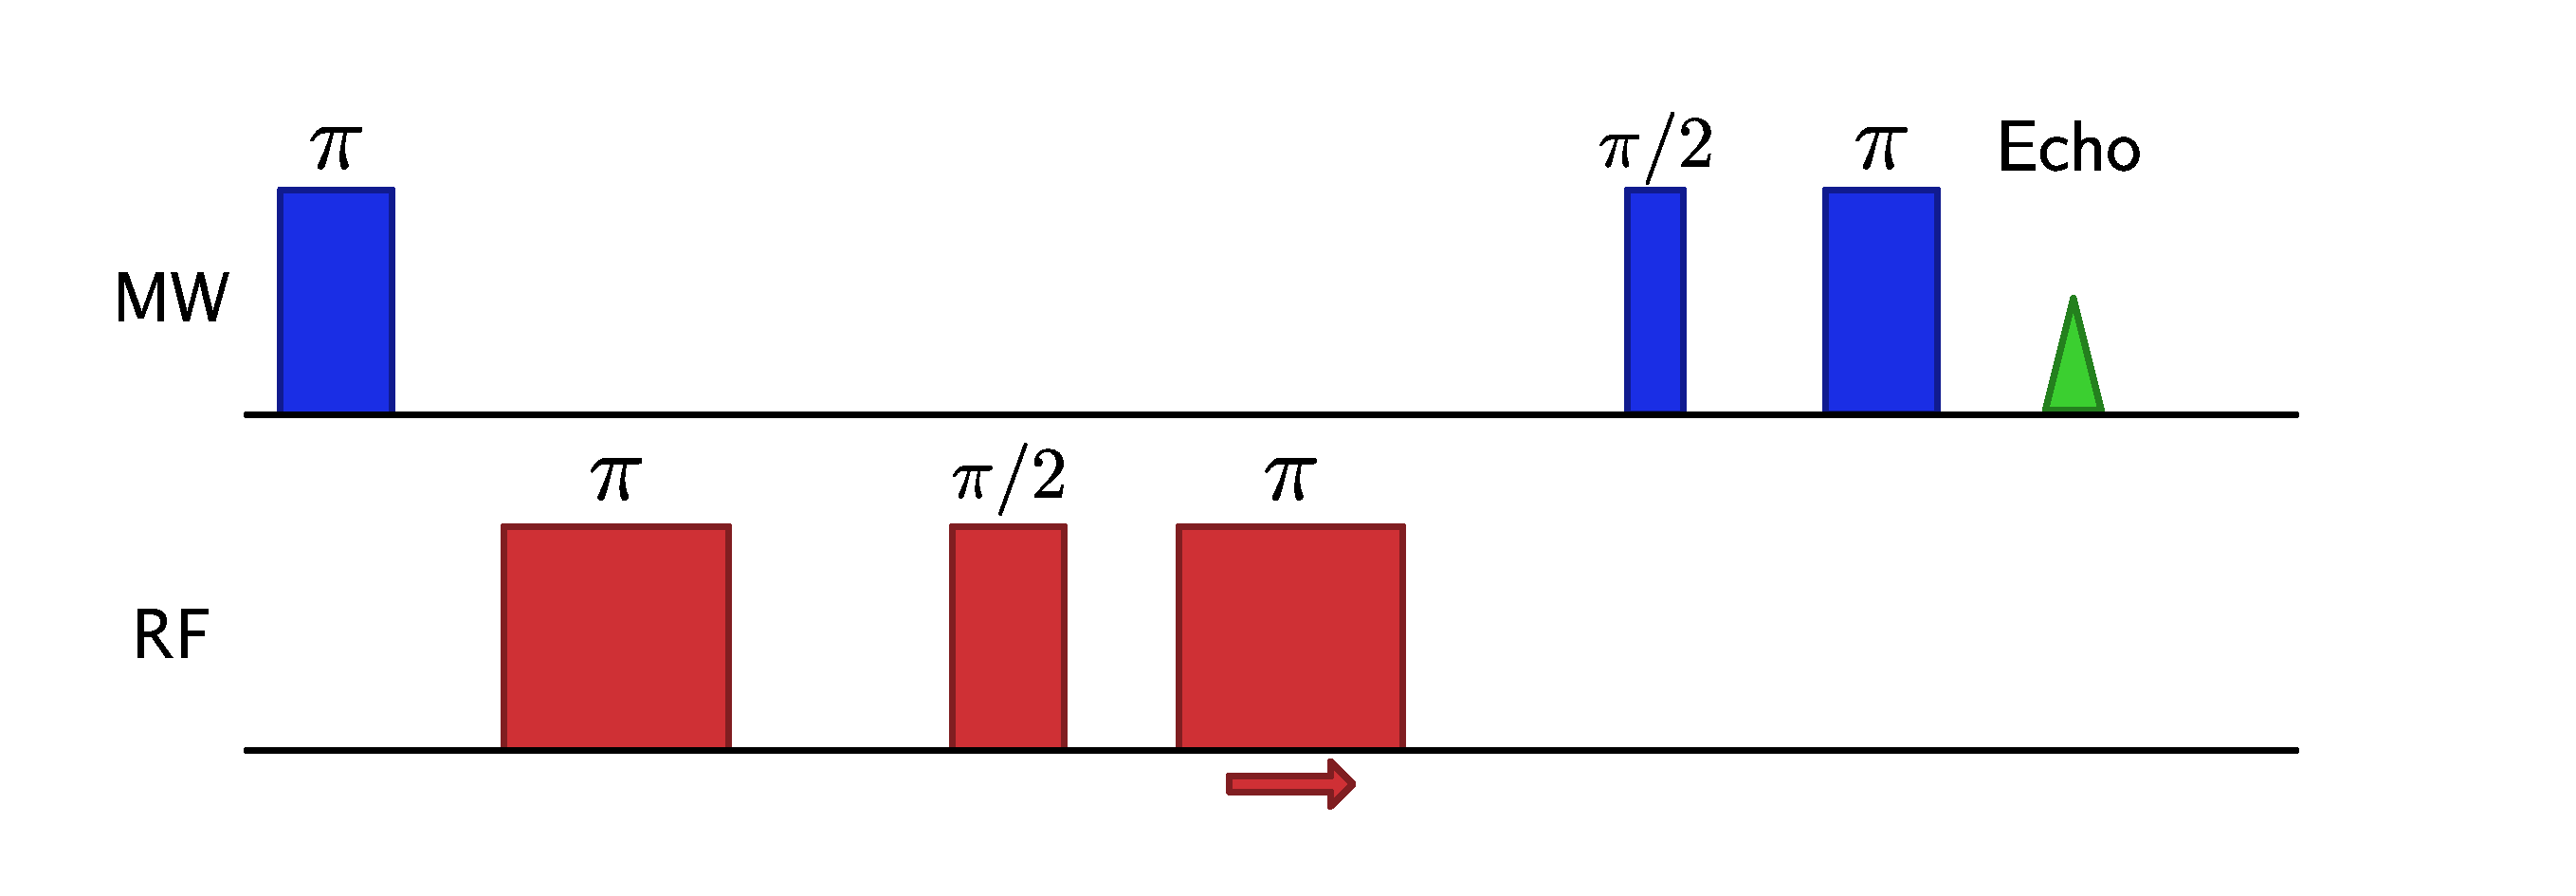
\includegraphics[width=\columnwidth]{Figures/NucEchoSequence2.pdf}
\caption[Nuclear echo pulse sequence]{Cartoon showing the pulse sequence for a nuclear spin echo}
\label{fig:nuclearecho}
\end{figure}

The nuclear echo sequence can be used to measure the Stark shift by setting the pulse intervals equal and adding a dipolar electric voltage pulse between two of the pulses.
This causes the nuclear spin to acquire phase depending on the length and strength of the voltage pulse.
If the voltage pulse length is swept whilst keeping all other factors constant then an oscillation of the signal is observed, giving the magnitude of the Stark shift.
\\
To measure nuclear $T_2$ time two pulse sequences can be used, with the most advantageous one being a full nuclear coherence transfer.
Whereas most ENDOR experiments only render the nuclear signal in one echo channel (real or imaginary) the full coherence transfer allows both to be meaningful.
It is also an important sequence as it allows the storage of quantum information in the nuclear spin, which has a much greater coherence time.
This opens up the possibility of using the nuclear spin as a memory for the electron spin \cite{Morton2008b}.

\begin{figure}
\centering
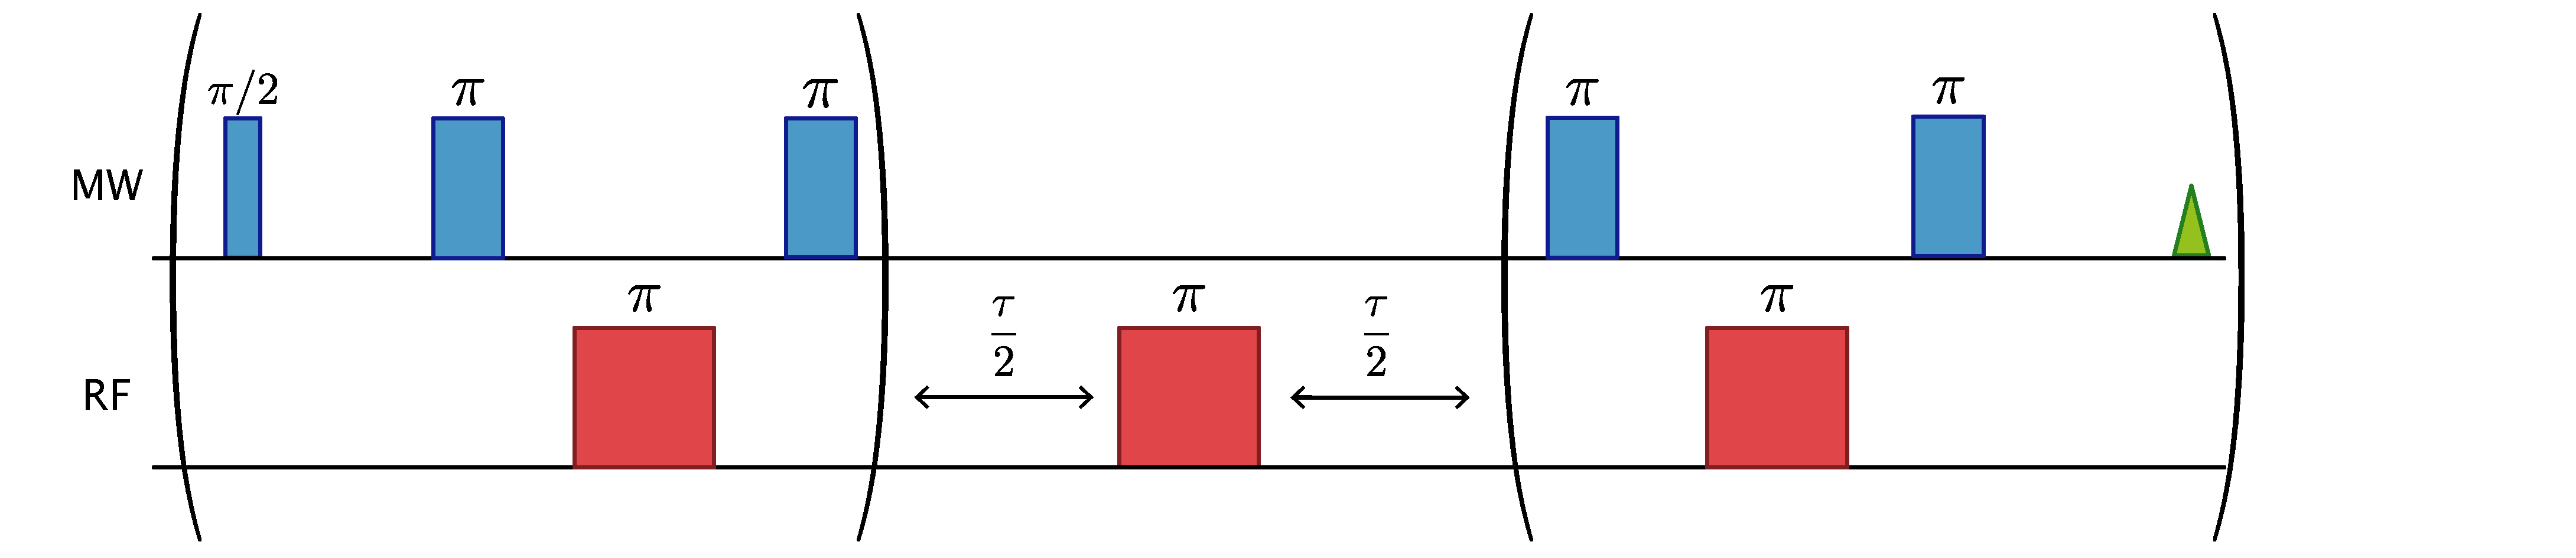
\includegraphics[width=\columnwidth]{Figures/fullcoherencetransfer.pdf}
\caption[Full coherence transfer]{Pulse sequence showing the full nuclear coherence transfer. Coherence is created by the first $\pi/2$ pulse before being transferred to the nuclear spin by the subsequent nuclear $\pi$ and electron $\pi$. After a set time the coherence is transferred back to the electron for read out.}
\label{fig:fullCoher}
\end{figure}

\section{Experimental Set-ups}
\subsection{Laser Experiments}
\label{sec:lasExps}

The set-up for measuring the impact of laser illumination on donors in silicon was relatively simple.
The measured sample is placed in a Bruker resonator and loaded into a helium flow cryostat.
The helium flow is initiated and the sample allowed to reach the desired temperature.
The Toptica laser beam is initially split using a $90/10$ beam-splitter, with the lower power beam subsequently coupled into a fibre.
Before fibre coupling the beam must be reflected off two adjustable mirrors to allow sufficient degrees of freedom for optimisation of power input.
The fibre passes into a wavemeter, used to determine the output wavelength, and is coarsely tuned to the desired wavelength.
The laser beam is not visible so is aligned to the cryostat window via an infrared-sensitive camera.
For fine-tuning of the alignment, two approaches were used.
The first is to place the sample in between two metallic contacts connected to a lock-in amplifier with a small oscillating voltage applied across the plates.
The laser spot location is fine tuned via adjustable mirrors until the current measured by the lock-in amplifier is maximised.
An alternative technique, not requiring the additional components but taking more time, is to maximise the effect of the laser.
This is done by measuring $T_1$ time of the sample repeatedly and adjusting the laser to minimise this measurement (indicating that the effect of the laser is maximised).
\\
The laser output power can be controlled by changing the amplitude of the control voltage.
This output power can be measured using a power metre and set to the desired value.
Although this approach is appropriate for high powers, the limited resolution of the power metre ($\approx$ 0.2mW) makes it inappropriate for lower powers.
To reach lower laser powers at reasonable errors ND filters are used.
These are valued from ND 1.0 - 4.0 and ND 0.1-0.6 in two separate filter wheels.
The power is set via control voltage to a stable value and ND filters are then used to adjust to the power at the sample.
Manufacturer values for transmission at the relevant wavelength are then used to calculate exact powers as these vary slightly with wavelength.
\\
In all experiments on laser illumination the sample used was a float zone natural silicon sample doped at $6\times10^{15}\text{cm}^{-3}$ and sized at $1.5\times1.5\times10$mm.

\subsection{Stark Shift Experiments}

The Stark shift measurement set-up requires placing the sample in between two copper electrodes designed to cover the sample.
The electrodes are placed in direct contact with the sample and held in place by thread tape.
These electrodes are each soldered to a copper wire allowing the application of voltage pulses.
Bi-polar pulses are generated using an AWG at up to $\pm2$V and subsequently amplified using an operational amplifier with a gain of $60\times$.
Pulses are simultaneously monitored on an oscilloscope during application to measure the exact voltage being applied.
For measurements on the $^{29}$Si nuclei temperatures of 4.5~K were used to ensure that the electron $T_1$ was long enough to ensure it did not restrict nuclear coherence times.
To reset the electron polarisation an infra-red LED is used at the base of the resonator to illuminate the sample when desired, effecting a rapid relaxation to thermal equilibrium.

% !TEX root = ../Thesis.tex
\chapter{Results}

In this chapter I will address the results gained so far. Looking first at the impact of laser illumination on coherence times before examining the impact of the Stark shift on selenium donors in purified silicon and the hyperfine coupling of phosphorus donors to $^{29}$Si nuclei in natural silicon.

\section{Illumination Induced Decoherence}

\subsection{Initial Measurements}

The first step undertaken before any laser illumination occurs is to characterise the sample's $T_1$ and $T_2$ times `in the dark' at the measurement temperature. 
Experiments were performed at 8~K and 7k, with typical $T_1$ and $T_2$ decays shown in figure \ref{fig:t1andt2}.
The inversion recovery has been fitted with a standard exponential decay whilst the $T_2$ decay has had a stretched exponential decay applied.
The time constants of these decays give the $T_1$ and $T_2$ times with errors in the fit used to establish errors in their values.
The stretched exponential decay of $T_2$ indicates the presence of spectral diffusion.
$T_2$ decays with dynamical decoupling applied do not have this stretch factor as they are isolated from spectral diffusion.
A problem with the results presented here is a variation in the time constant for the decay in the dark, with 2.8~ms found in the high power experiments, whilst 6.4~ms was found during the low power experiments.
According to simulations and literature results this difference in $T_1$ would correspond to a temperature difference of approximately 0.3~K \cite{Tyryshkin2012}. 
These results are therefore presented separately to avoid confusion.
It is possible that this is attributable to different flow rates in the helium cryostat, meaning that use of a dry cryostat, which offers much greater temperature precision, would be beneficial. 
At 7~K $T_1$ was $32\pm0.1$ms and $T_2$ was unchanged.


\begin{figure}
\centering
\begin{subfigure}[b]{0.5\textwidth}
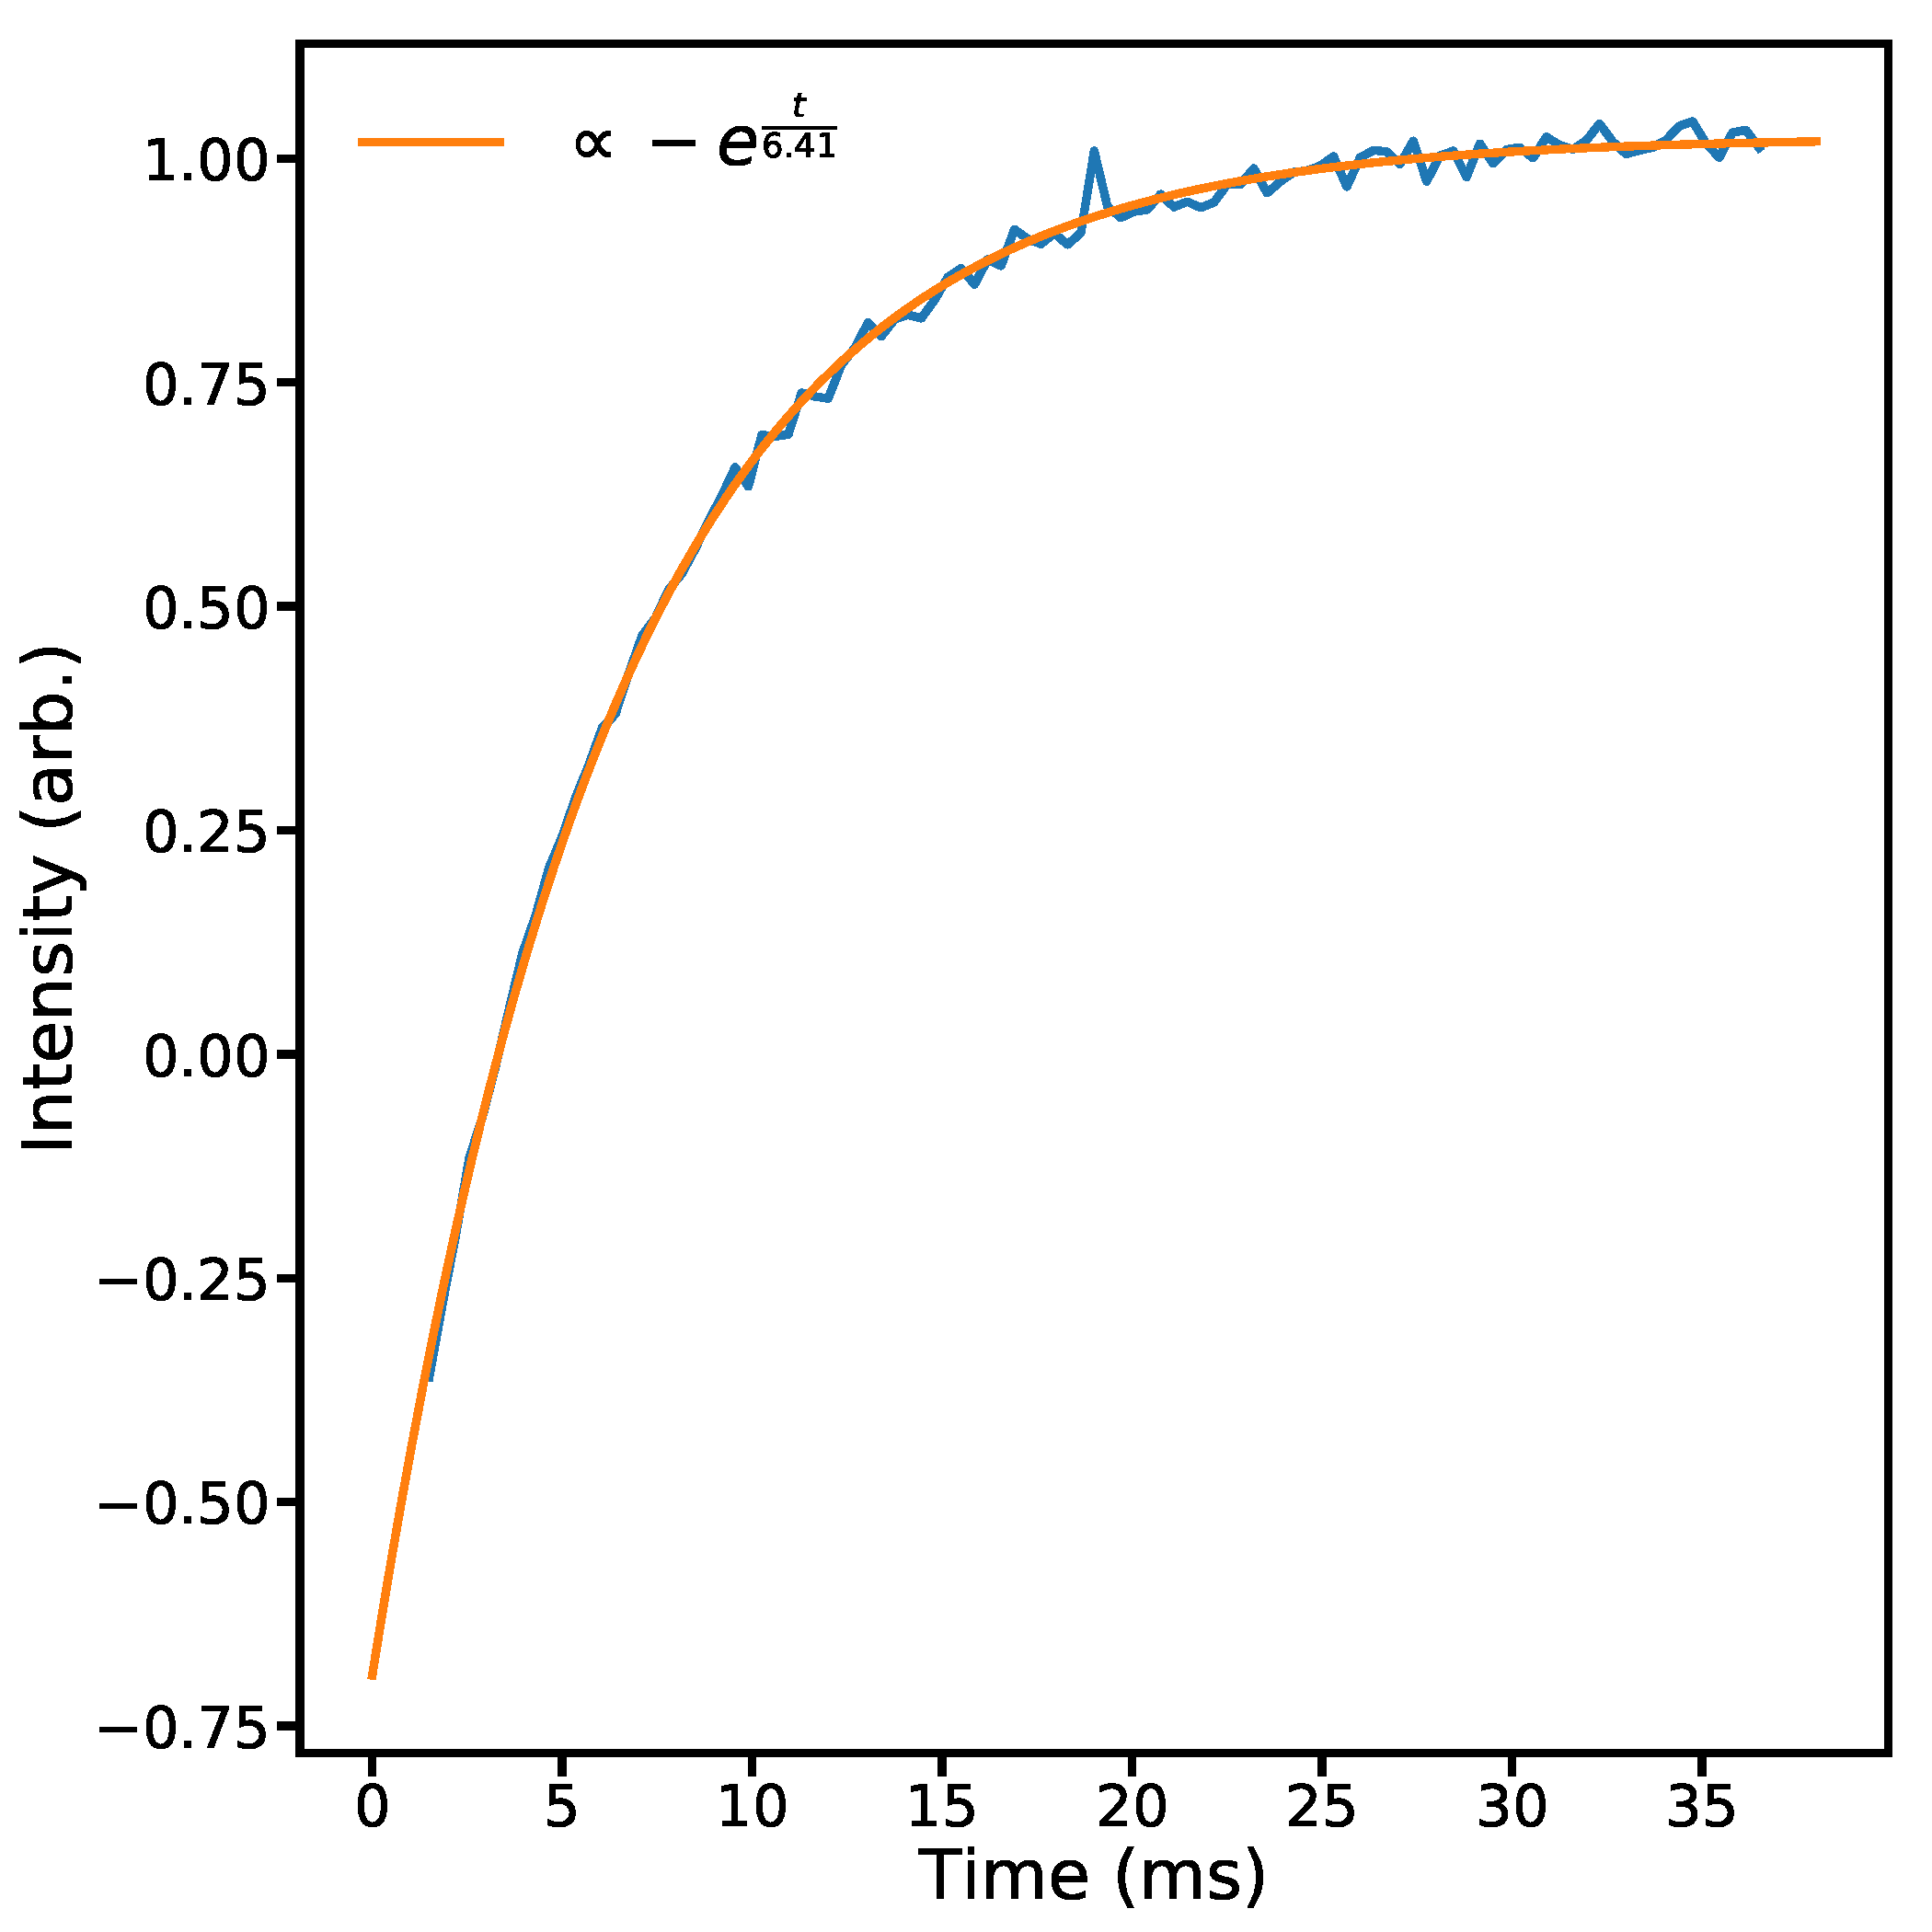
\includegraphics[width=\columnwidth]{Figures/T1Dark.pdf}{(a)}
\end{subfigure}%
\begin{subfigure}[b]{0.5\textwidth}
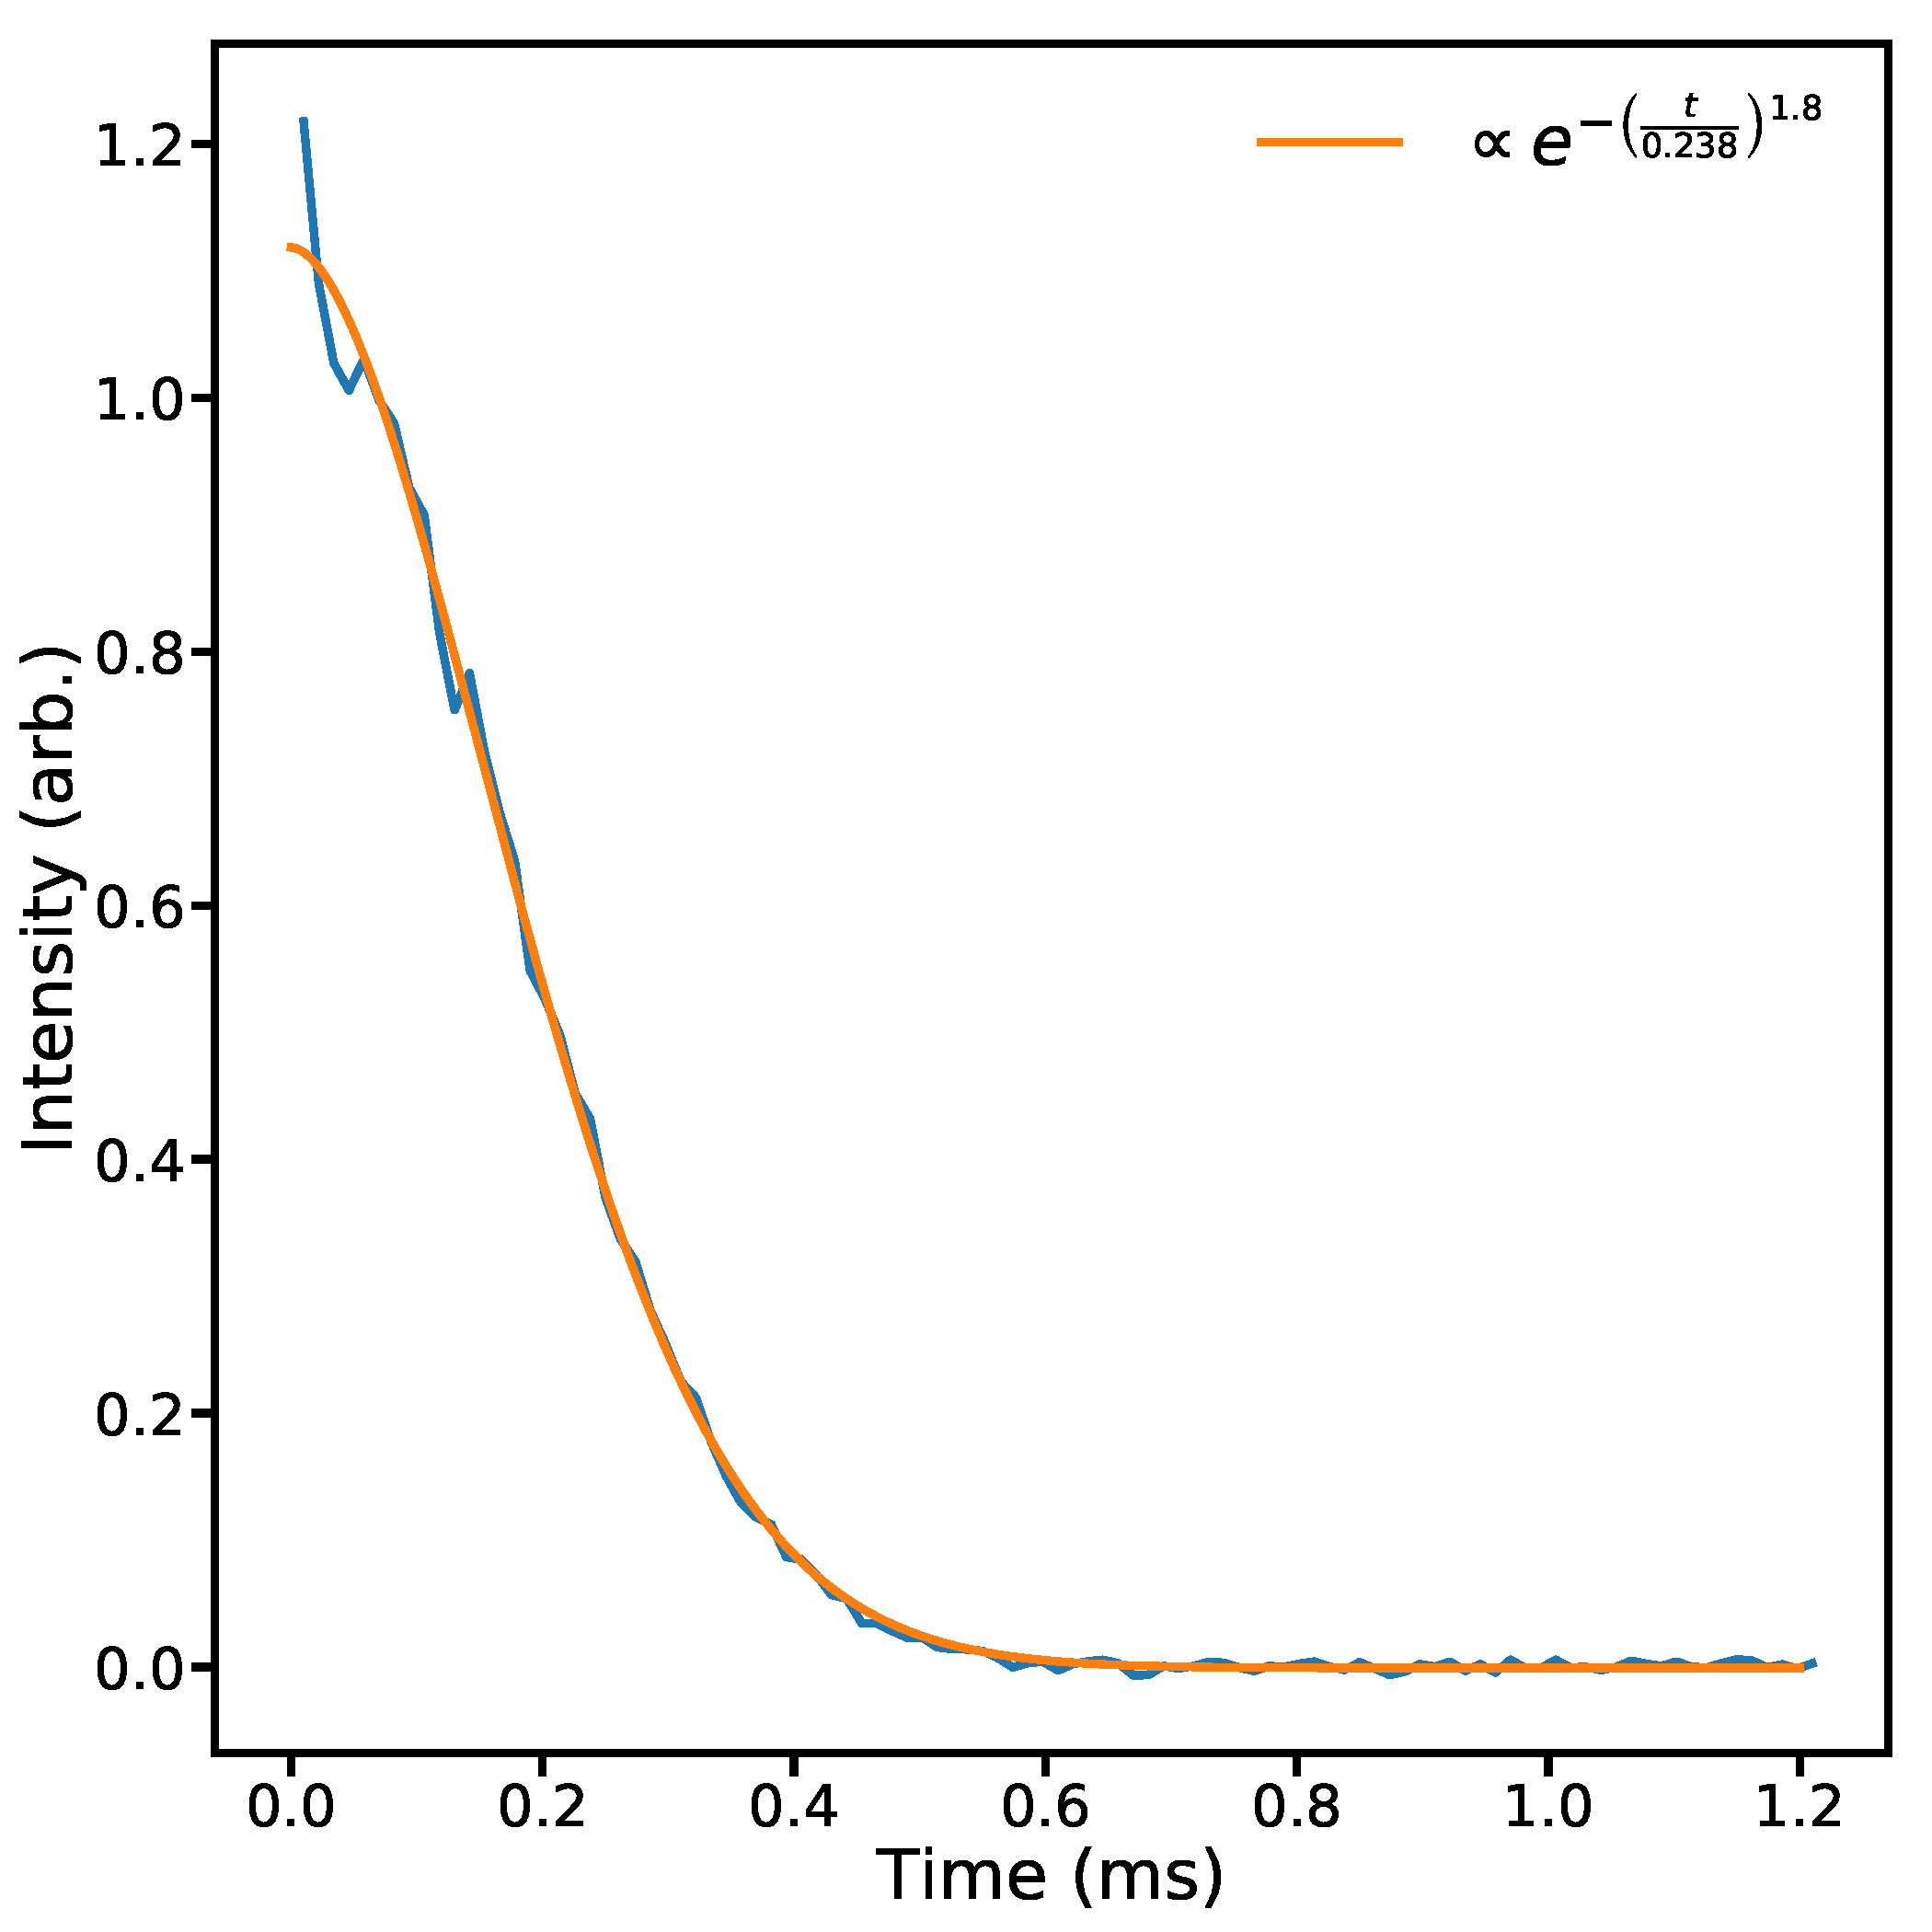
\includegraphics[width=\columnwidth]{Figures/T2Dark.pdf}{(b)}
\end{subfigure}%
\caption[$T_1$ and $T_2$ decays]{Typical $T_1$ and $T_2$ decays showing the inversion recovery for $T_1$ and the characteristic stretched exponential for $T_2$, indicating the presence of spectral diffusion.}
\label{fig:t1andt2}
\end{figure}

\subsection{Bi-Exponential Inversion Recovery}

A set of high power measurements have been taken at powers between 2~mW and 130~mW, at wavelengths 1058~nm, 1070~nm and 1080~nm, and at temperatures of 7~K and 8k.
At each power and wavelength 3 measurements were made: $T_1$, $T_2$ and $T_2$ whilst using a 4 $\pi$ pulse dynamical decoupling sequence - CPMG-4 \cite{Carr1954}.
An initial observation is that the inversion recovery is best fit by a bi-exponential (rather than a single exponential) of the form:

\begin{equation}
a e^{\frac{t}{T_{1a}}} + b e^{\frac{t}{T_{1b}}}
\end{equation}

this is clearly seen in figure \ref{fig:biexpDec}.

\begin{figure}
\centering
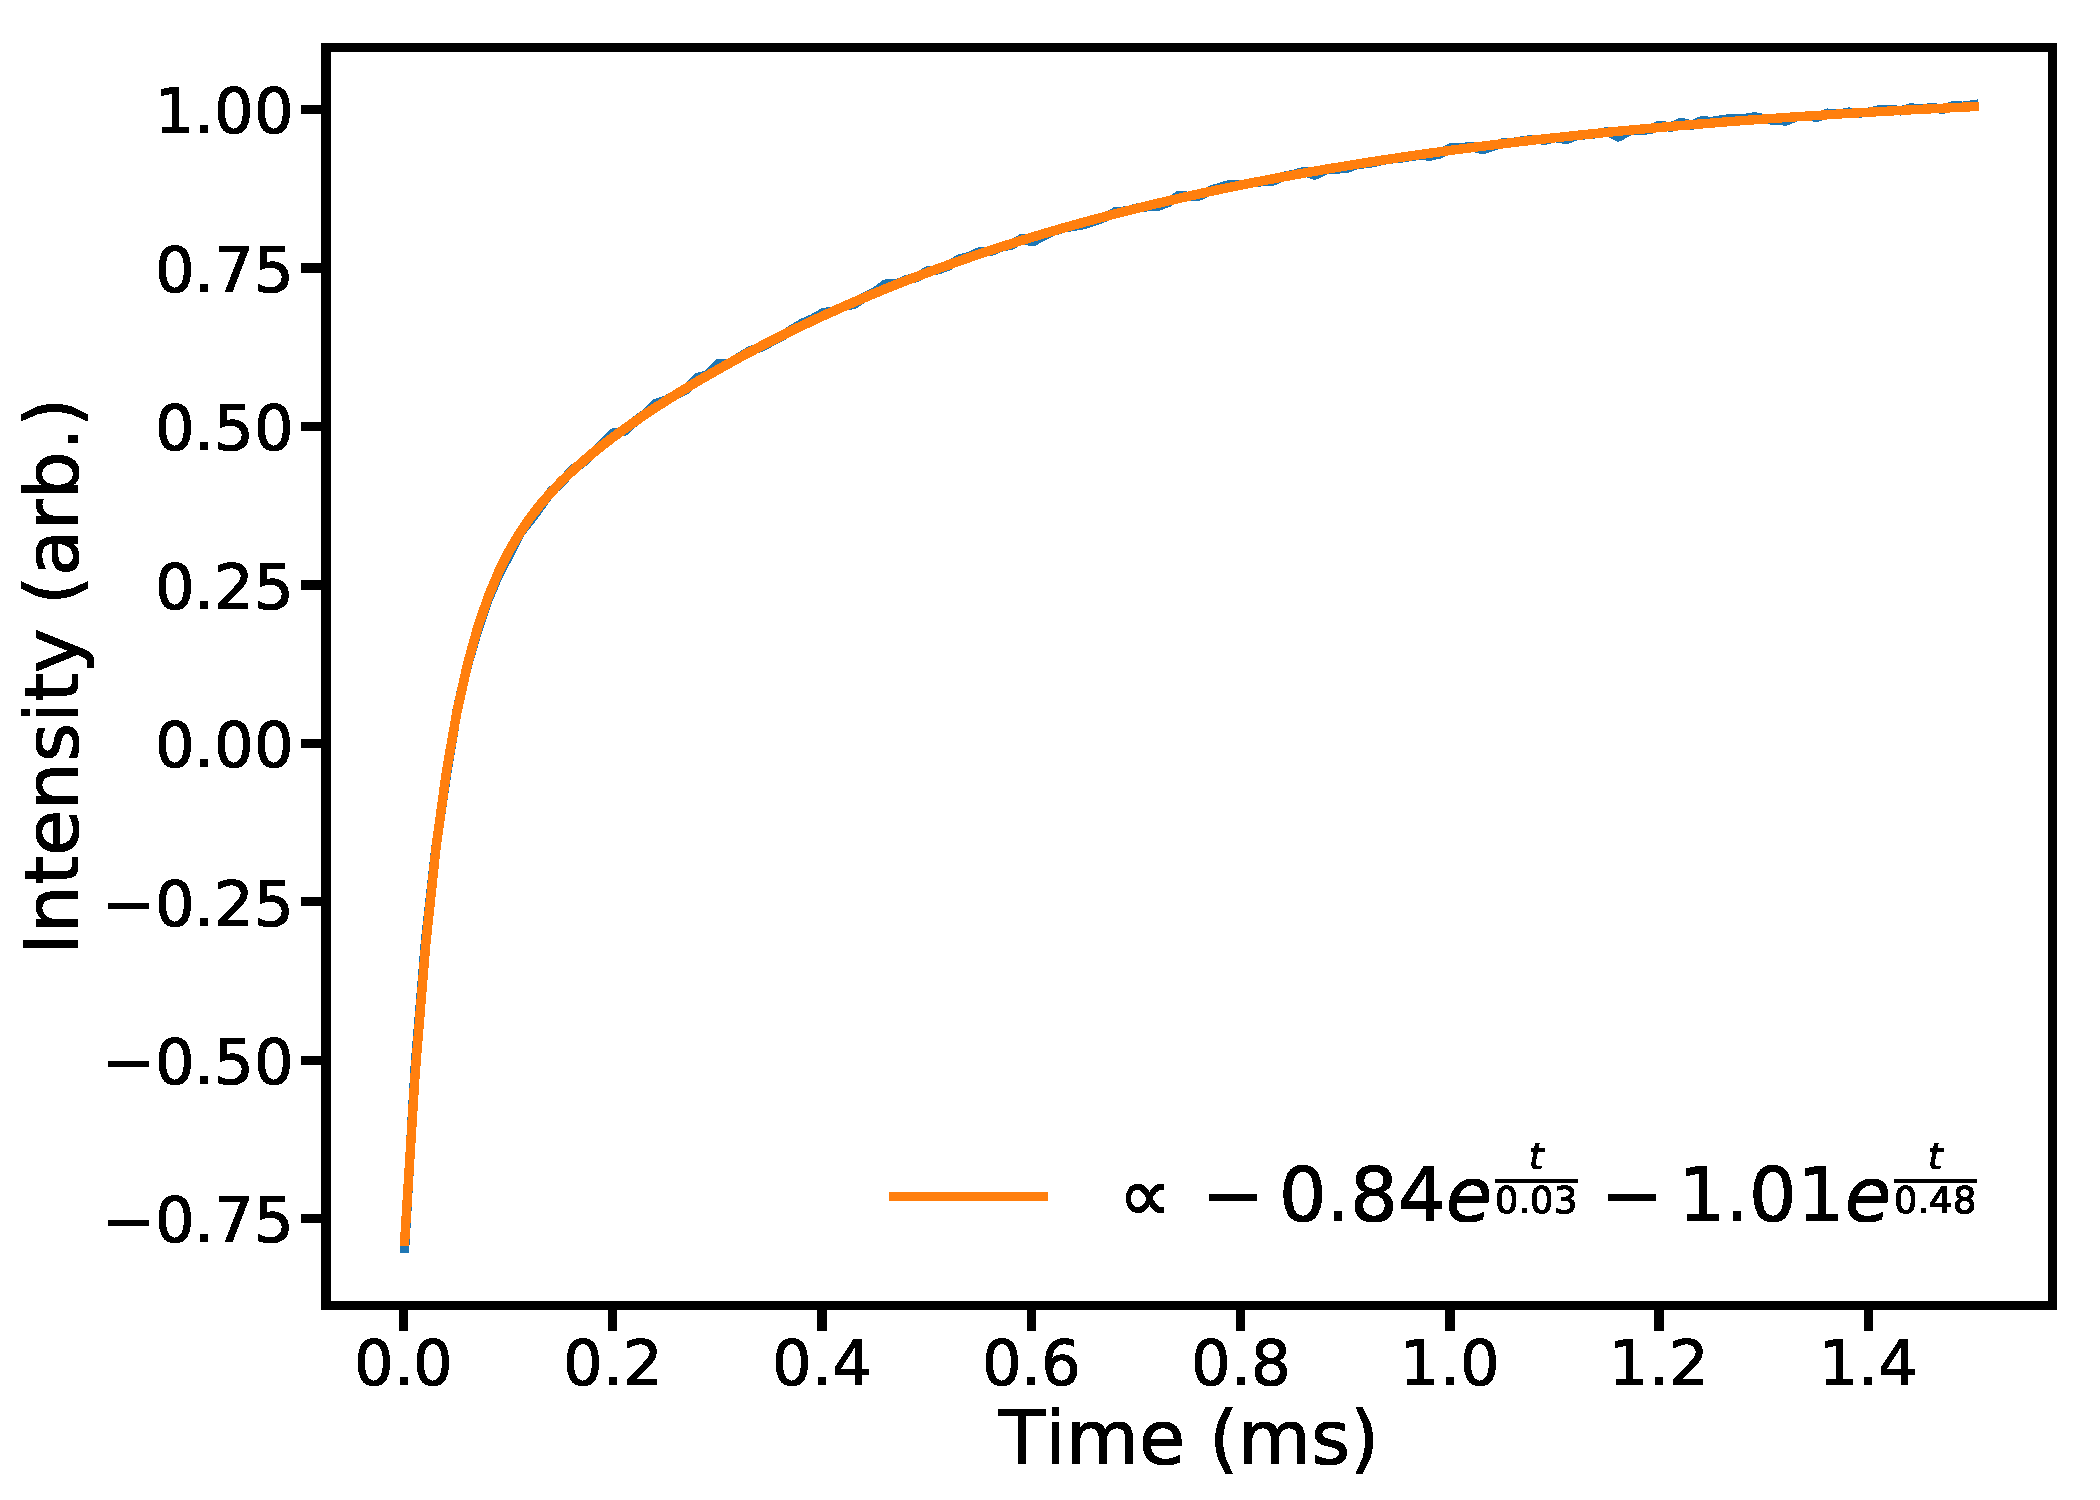
\includegraphics[width=0.8\textwidth]{Figures/T1_biExp.pdf}
\caption[Inversion recovery under laser illumination]{Inversion recovery at 8~K and under 79~mW illumination at 1070~nm. Of note is the strongly bi-exponential nature of the decay, with two distinct time constants describing it. One significantly longer than the other. A possible explanation for this is that the laser illumination is not affecting all parts of the sample. This is not unexpected as the sample is quite large, as described in section \ref{sec:lasExps}}. 
\label{fig:biexpDec}
\end{figure}

Of the two time constants that describe the decay, one is significantly longer than the other and at low powers is close to the $T_1$ in the dark.
This suggests that there is a distribution of the illumination effect throughout the sample, with less affected parts relaxing more slowly than others. 
This becomes more obvious when comparing the two time constants over a range of powers, as seen in figure \ref{fig:T1avsT1b}.
This shows that the shorter $T_1$ has a strict inverse polynomial dependence on laser power, whilst the longer $T_1$ cannot be similarly fit as it appears to saturate at lower powers.
Given this, it seems prudent when trying to determine the relationship between the incident light parameters and relaxation behaviour to use the shorter of the two time constants where a bi-exponential fit has been applied.
In the case of a set of data qubits close to the silicon surface, as is suggested in \cite{OGorman2014}, these qubits would be exposed to illumination and not shielded as appears to be the case for donors experiencing the long $T_1$.



\begin{figure}
\centering
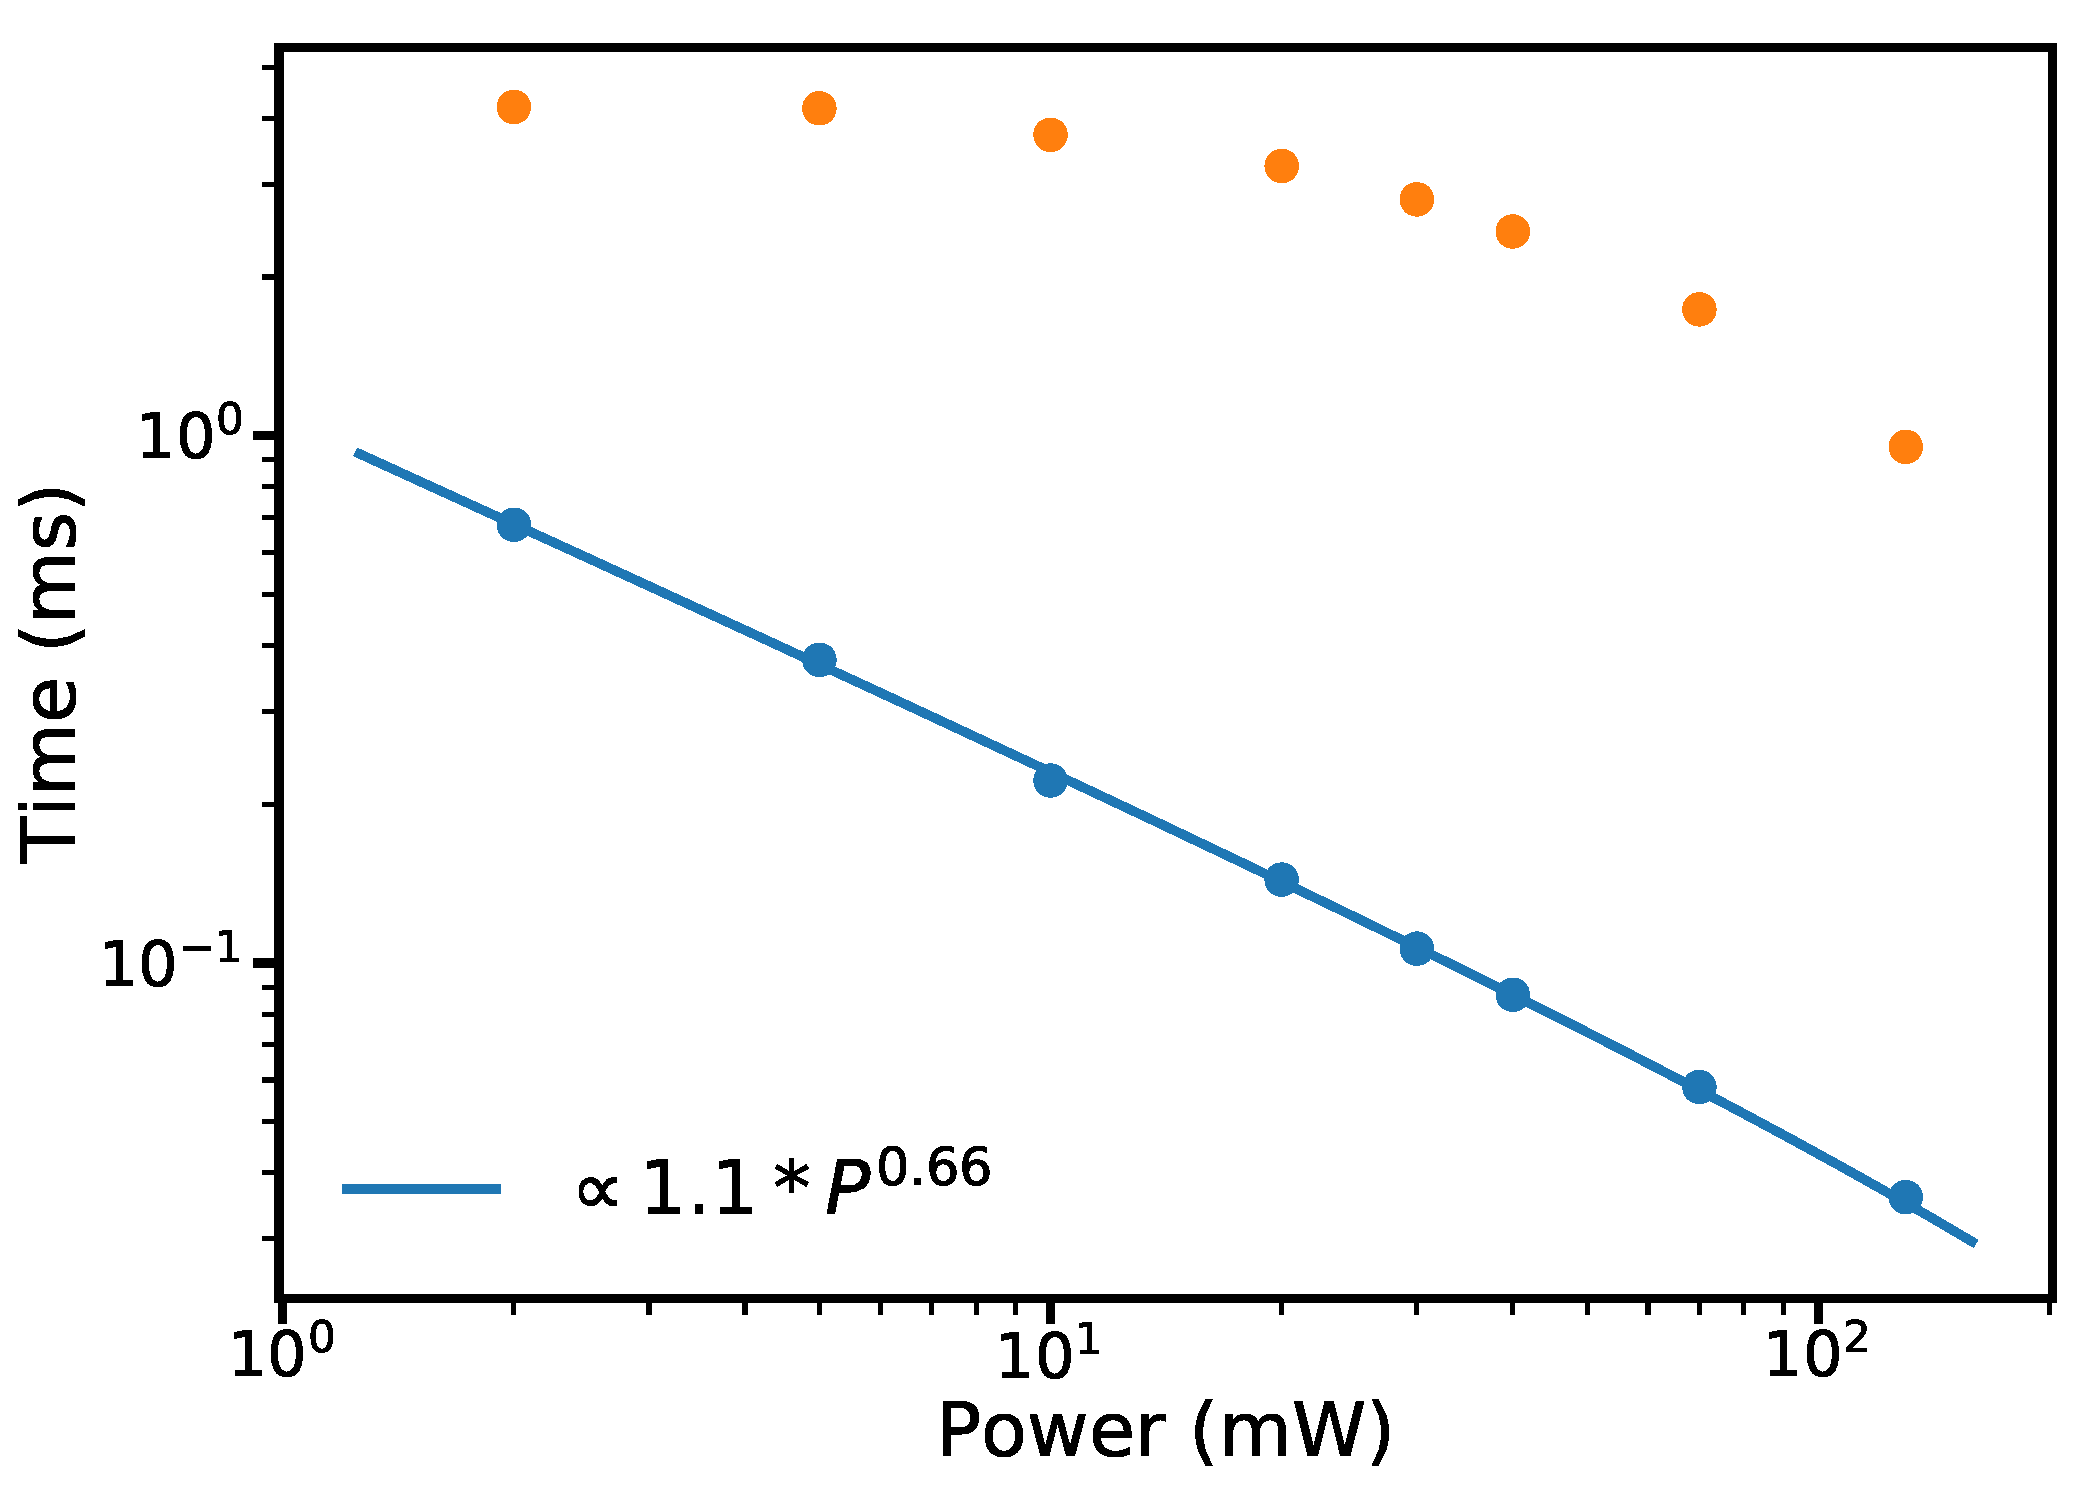
\includegraphics[width = 0.8\columnwidth]{Figures/hpT1avsT1b.pdf} 
\caption[Bi-exponential relaxation decay constants]{Figure shows the two time constants for bi-exponential relaxation decay whilst under laser illumination at 1070~nm and at 8k. The shorter $T_1$ constant is well fit with a $\frac{1}{P^{0.66}}$ line. A similar fit cannot be applied to the longer $T_1$ constant, which appears to demonstrate saturation behaviour at the lower illumination powers.}
\label{fig:T1avsT1b}
\end{figure}

\subsection{High Power Wavelength Comparison}
\subsubsection{Effect on $T_1$}

Measurements comparing behaviour of $T_1$, $T_2$ and dynamical decoupling $T_2$ were performed at 3 wavelengths: 1058~nm, 1070~nm, and 1080~nm.
The shortest of these represents photon energies at approximately the band gap energy of silicon. 
As such, it would be expected that this wavelength would have a stronger effect than the other two as the free carrier generation rate would be significantly higher.
This factor has previously been postulated as the dominant process affecting relaxation rates of donor electrons.
Figure \ref{fig:wavcomparison} shows the relationship between relaxation time and laser power for three wavelengths, fitted according to $A/t^{\alpha}$. 
This fit is applied due to the expected relationship between power and photon density at the sample being approximately $\frac{1}{x}$. 
The observation that the relationship between power and $T_1$ time is close to linear on a log-log graph also suggests that it is based upon a power law.
The power for each wavelength is $0.73\pm.002, 0.68\pm.0002$ and $0.68\pm.003$, in order of increasing wavelength.
Measurements were also taken at 2~mW and 5~mW but are not included here as the large error in the power values makes them unsuitable for comparison between data sets. 
What is clear from the above graph is that there is an observable difference between the case of 1058~nm illumination and the two higher wavelengths. 
This is to be expected given that 1058~nm is at approximately the silicon band gap, meaning that absorption of photons will be higher and free carrier generation significantly higher than with less energetic photons.
Although the higher wavelengths have a lesser effect, there is still a strong reduction in relaxation times.
The similarity between the effects suggest that the mechanisms responsible for the increased rate do not have a strong dependence on individual photon energy once the band-gap is passed, instead the power of the incident illumination is dominant. 

\begin{figure}
\centering
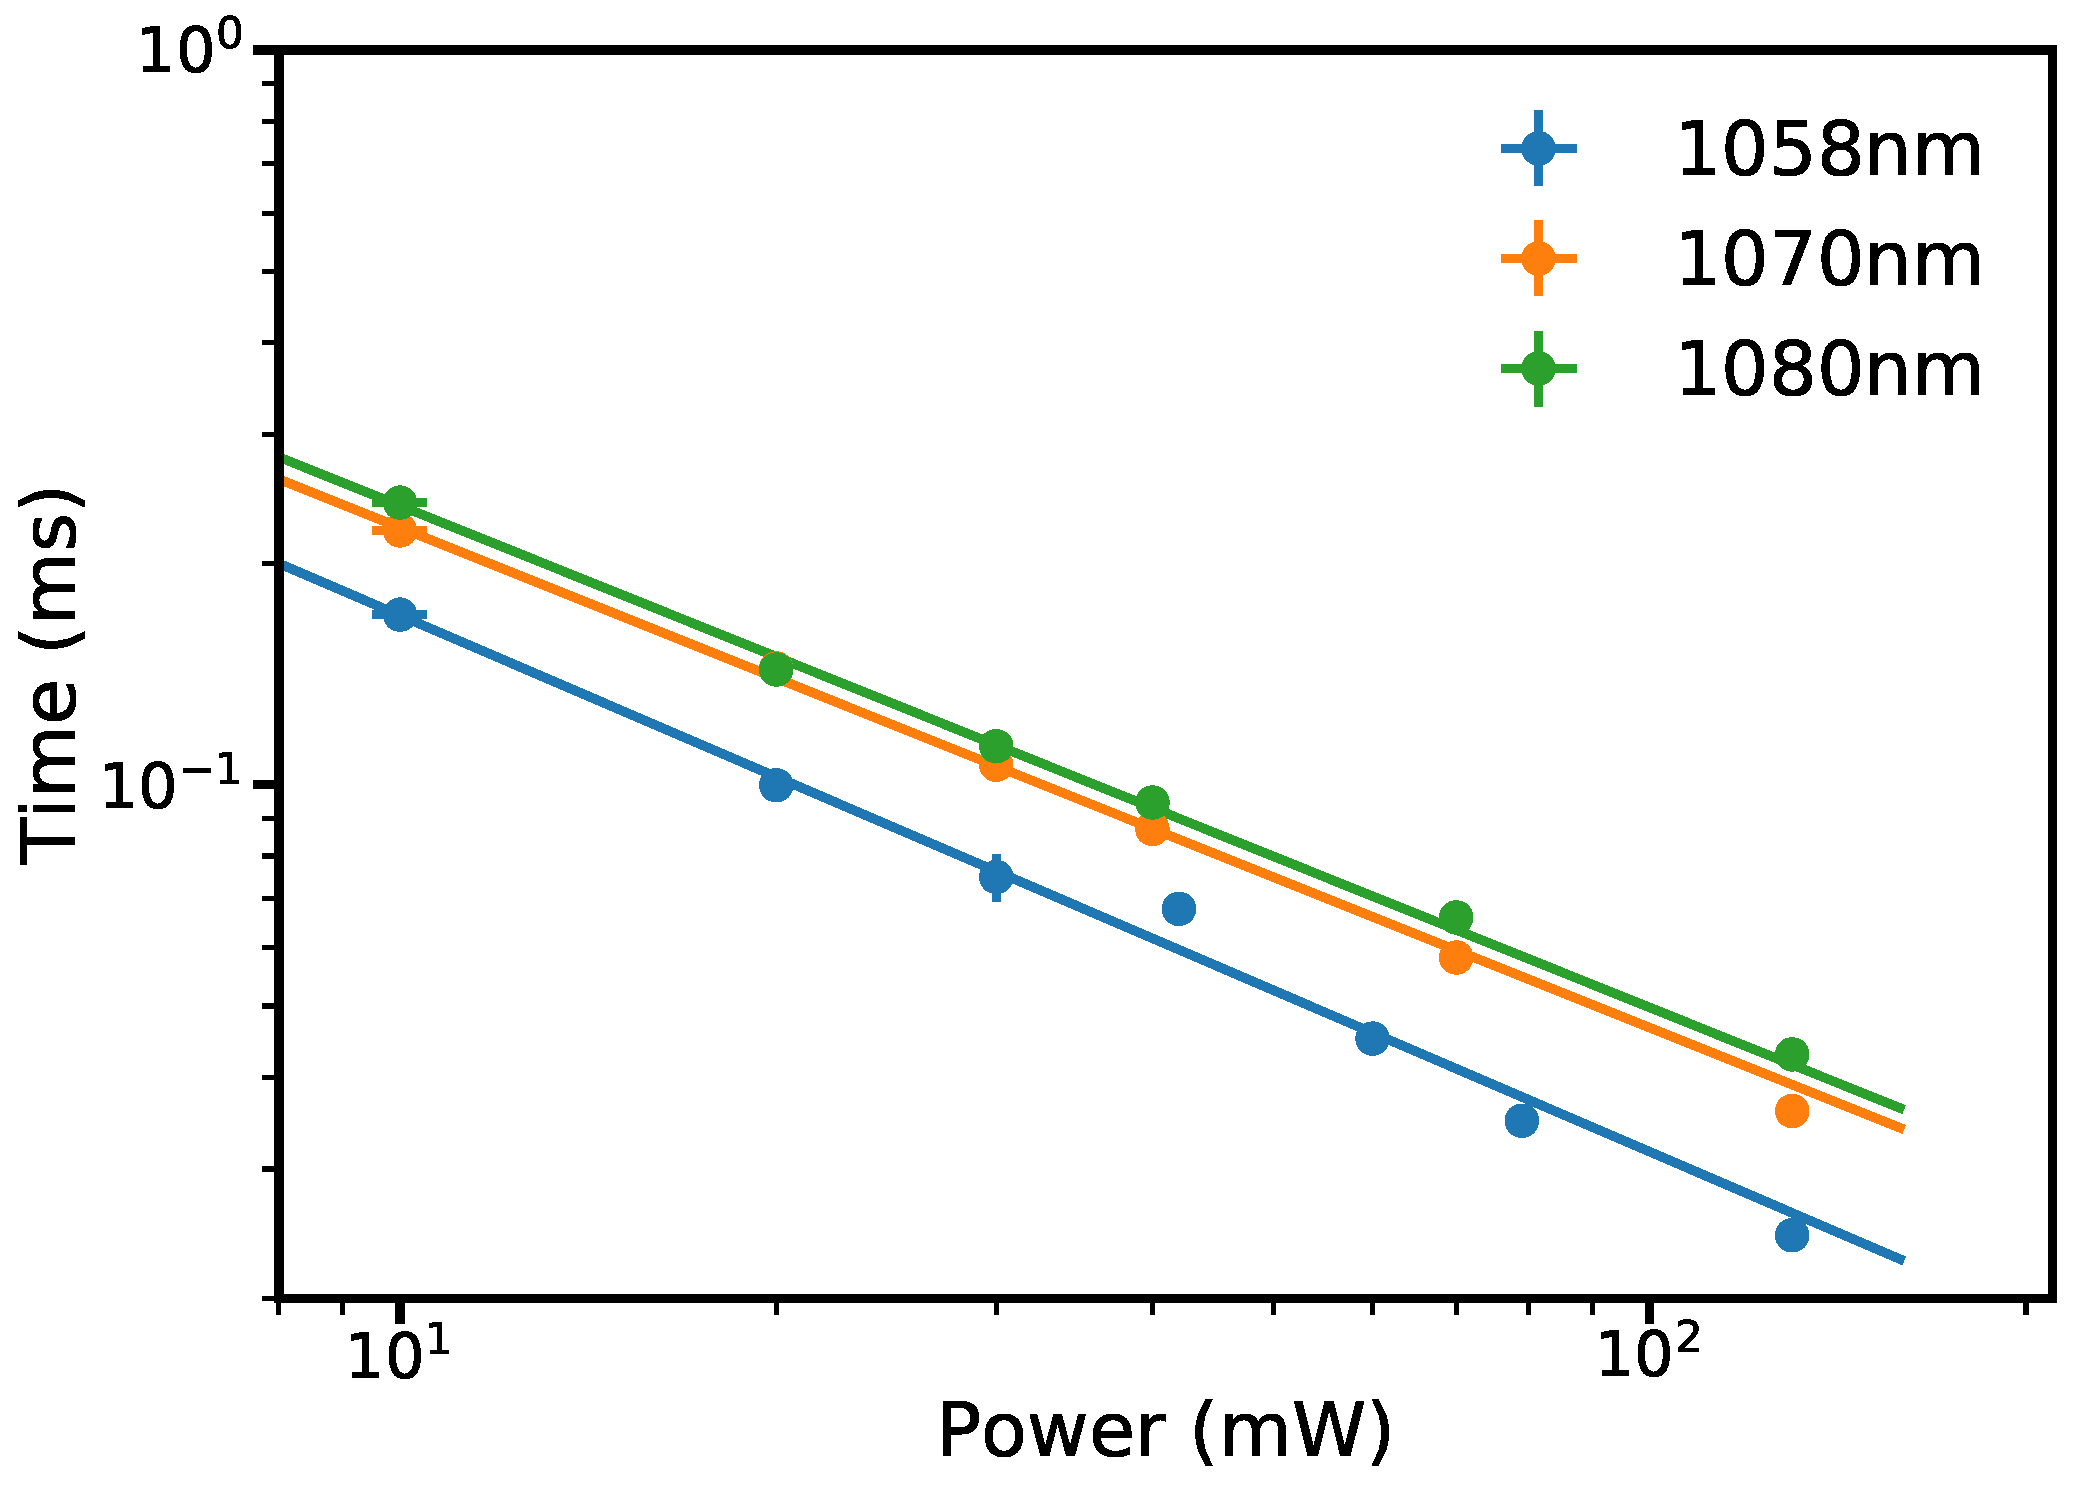
\includegraphics[width = 0.8\columnwidth]{Figures/Logwavelengthcomp.pdf}
\caption[Relaxation comparison at 8~K and 1058~nm, 1070~nm, and 1080~nm illumination]{Figure shows the relationship between laser power and relaxation time for 3 different wavelengths: 1058~nm, 1070~nm and 1080~nm.}
\label{fig:wavcomparison}
\end{figure}

The impact of illumination on relaxation rates observed here is in line with predictions.
Increased wavelength results in a slower relaxation rate at equivalent powers, with a more significant change being observed as the silicon band gap energy is crossed.
Relaxation rates follow a $a/P^{\alpha}$ curve.

\subsubsection{Effect on $T_2$}

Whilst the $T_1$ time is important for quantum information processing, as it ultimately limits computation time, $T_2$ is in most cases the limiting factor in qubit coherence.
The mechanisms that limit $T_2$ in spins were discussed in section \ref{sec:litdecoherence}.
Of particular worry is that a significant number of free electrons in the silicon conduction band could create time dependent magnetic fields at the observed donor spins. 
If this is the case then there could be an impact on the $T_2$ time beyond the effect of reduced $T_1$.
Figure \ref{fig:t1vst2wav} shows how $T_1$ and $T_2$ vary with laser power for 1058~nm and 1070~nm.
What is clear in both cases is that there does not appear to be a significant effect beyond $T_2$ being limited by $T_1$.
In both graphs it is clear at the lower powers that $T_2$ is beginning to saturate to the value in the dark of $220\mu$s.
The fact that there is no clear difference between the effects in the 1058~nm case and the 1070~nm case is interesting. 
It suggests that, although there is clearly a greater magnitude of effect in the lower wavelength case, if the mechanism is different then it has no impact on $T_2$ above and beyond the extra $T_1$ limitation.


\begin{figure}
\centering
\begin{subfigure}[b]{0.5\columnwidth}
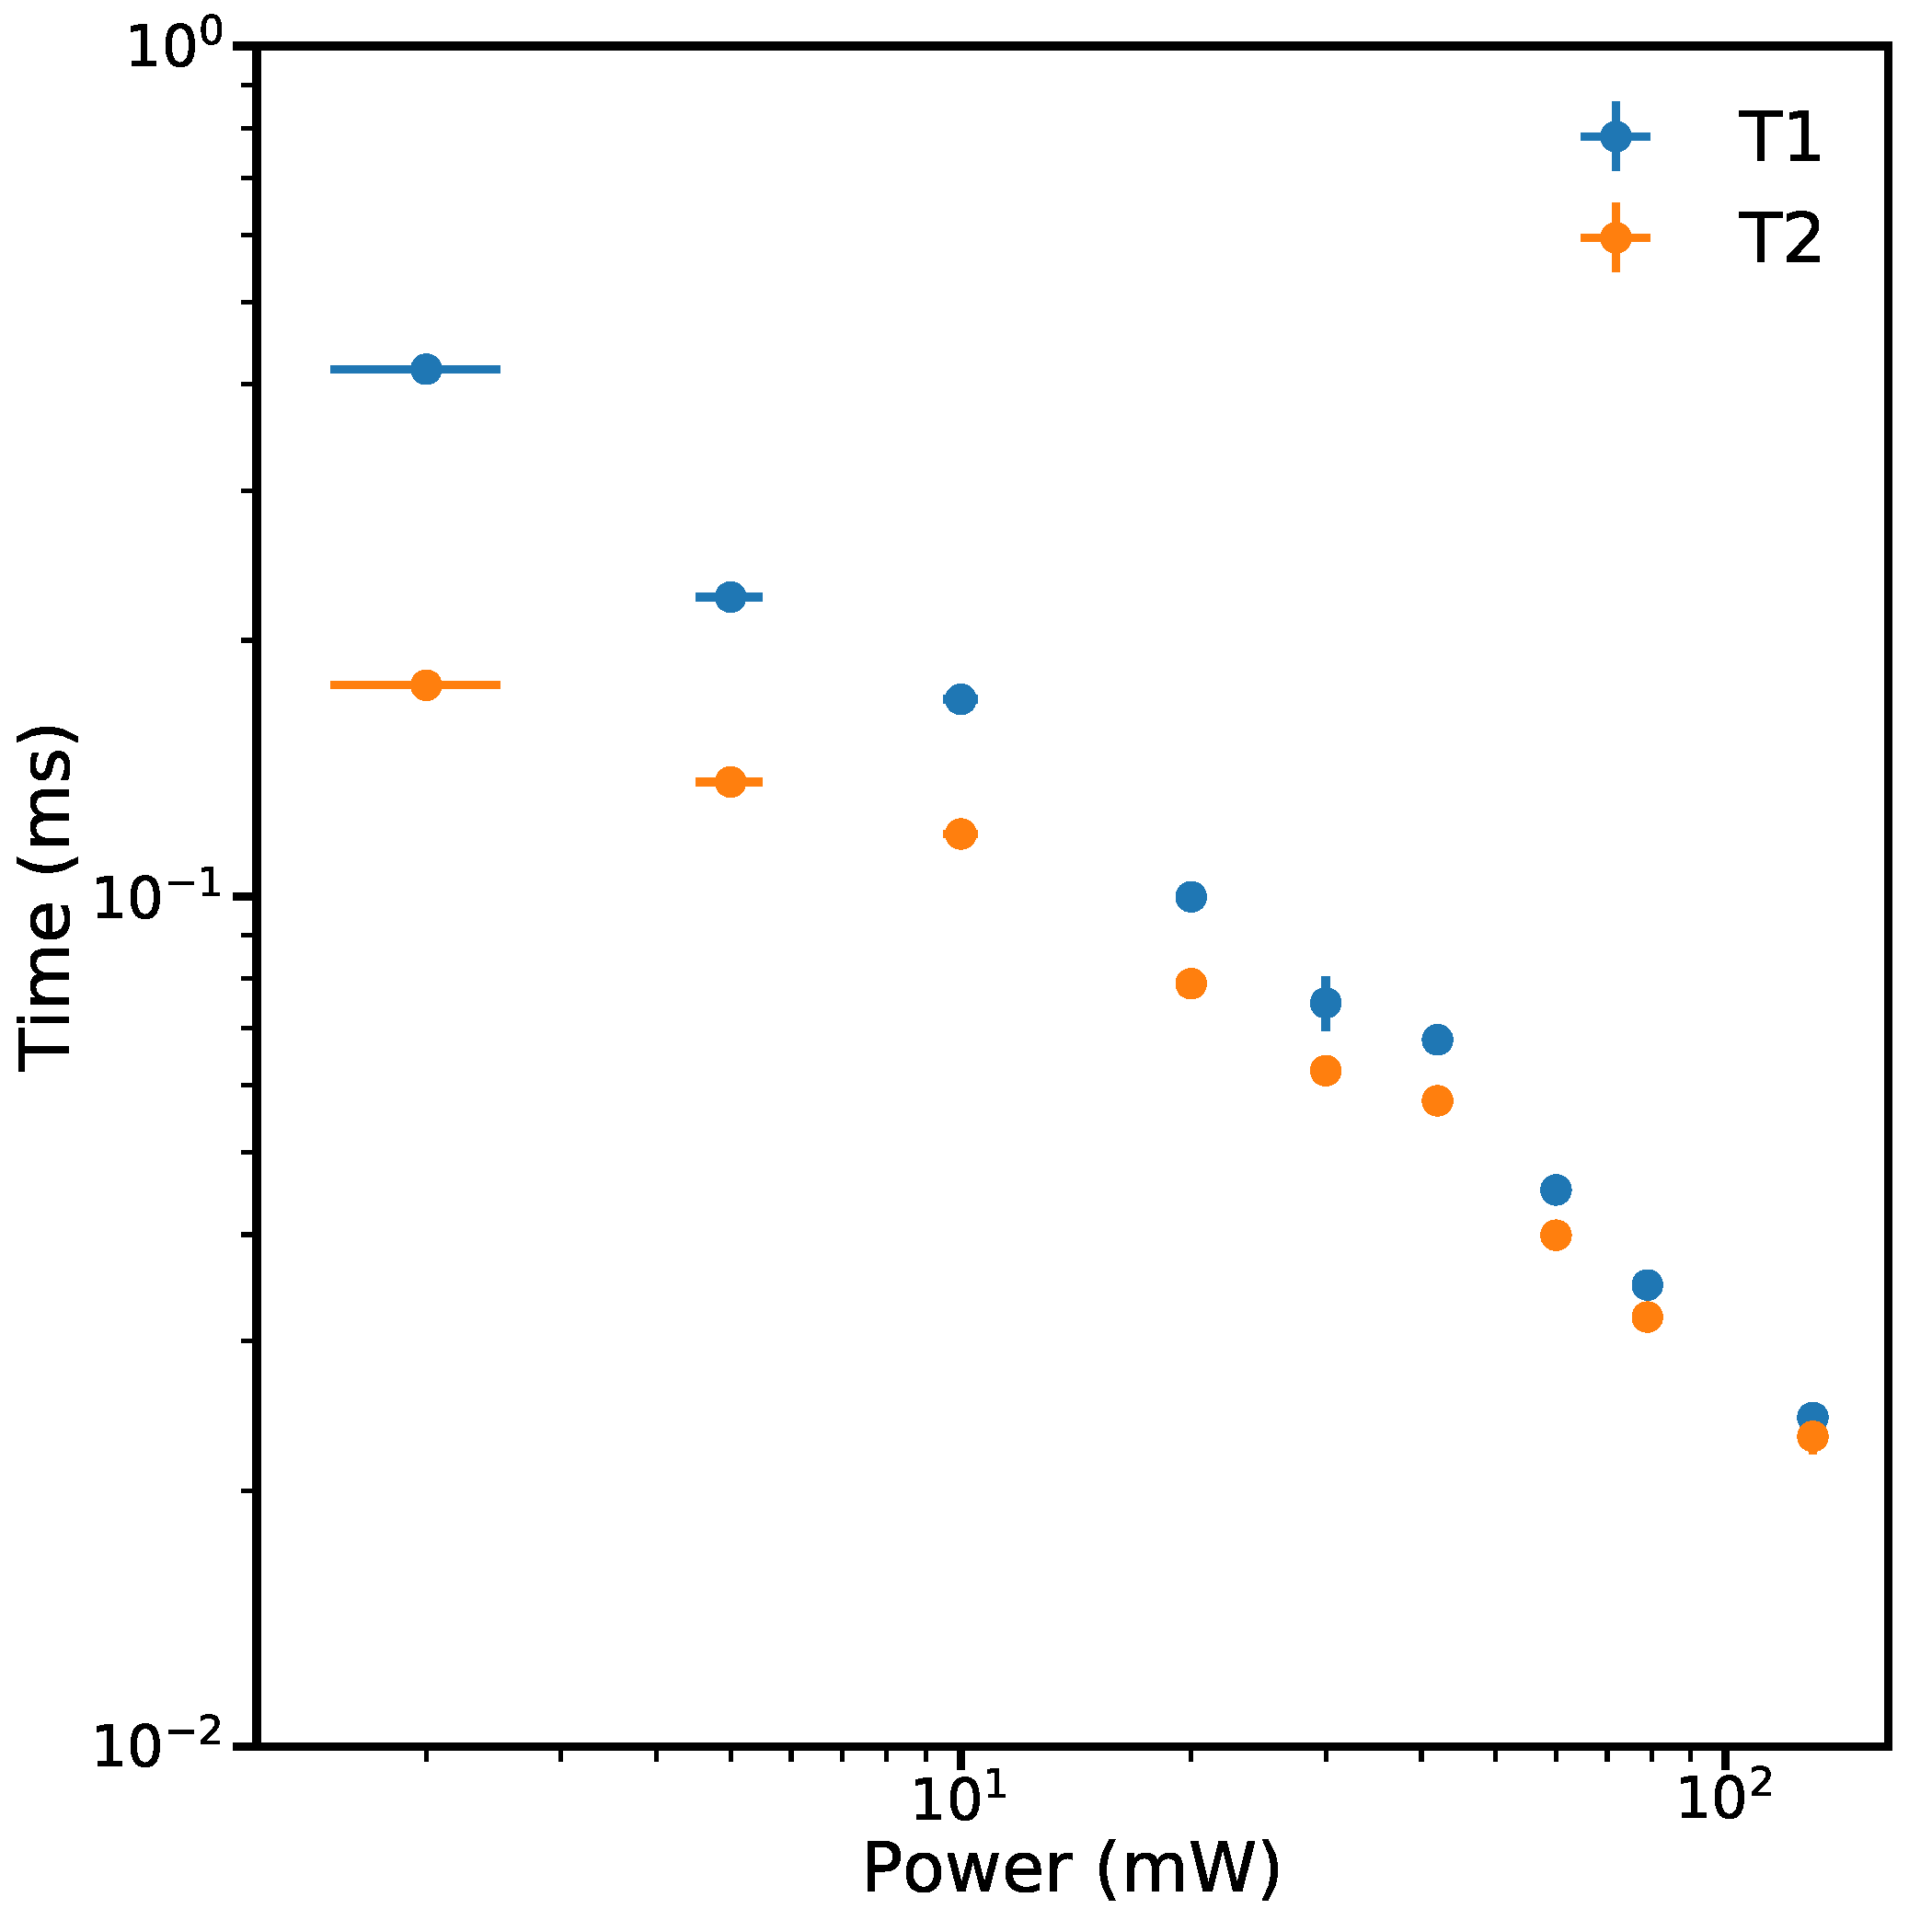
\includegraphics[width = \columnwidth]{Figures/8kT1vsT21058.pdf}{(a)}
\end{subfigure}%
\begin{subfigure}[b]{0.5\columnwidth}
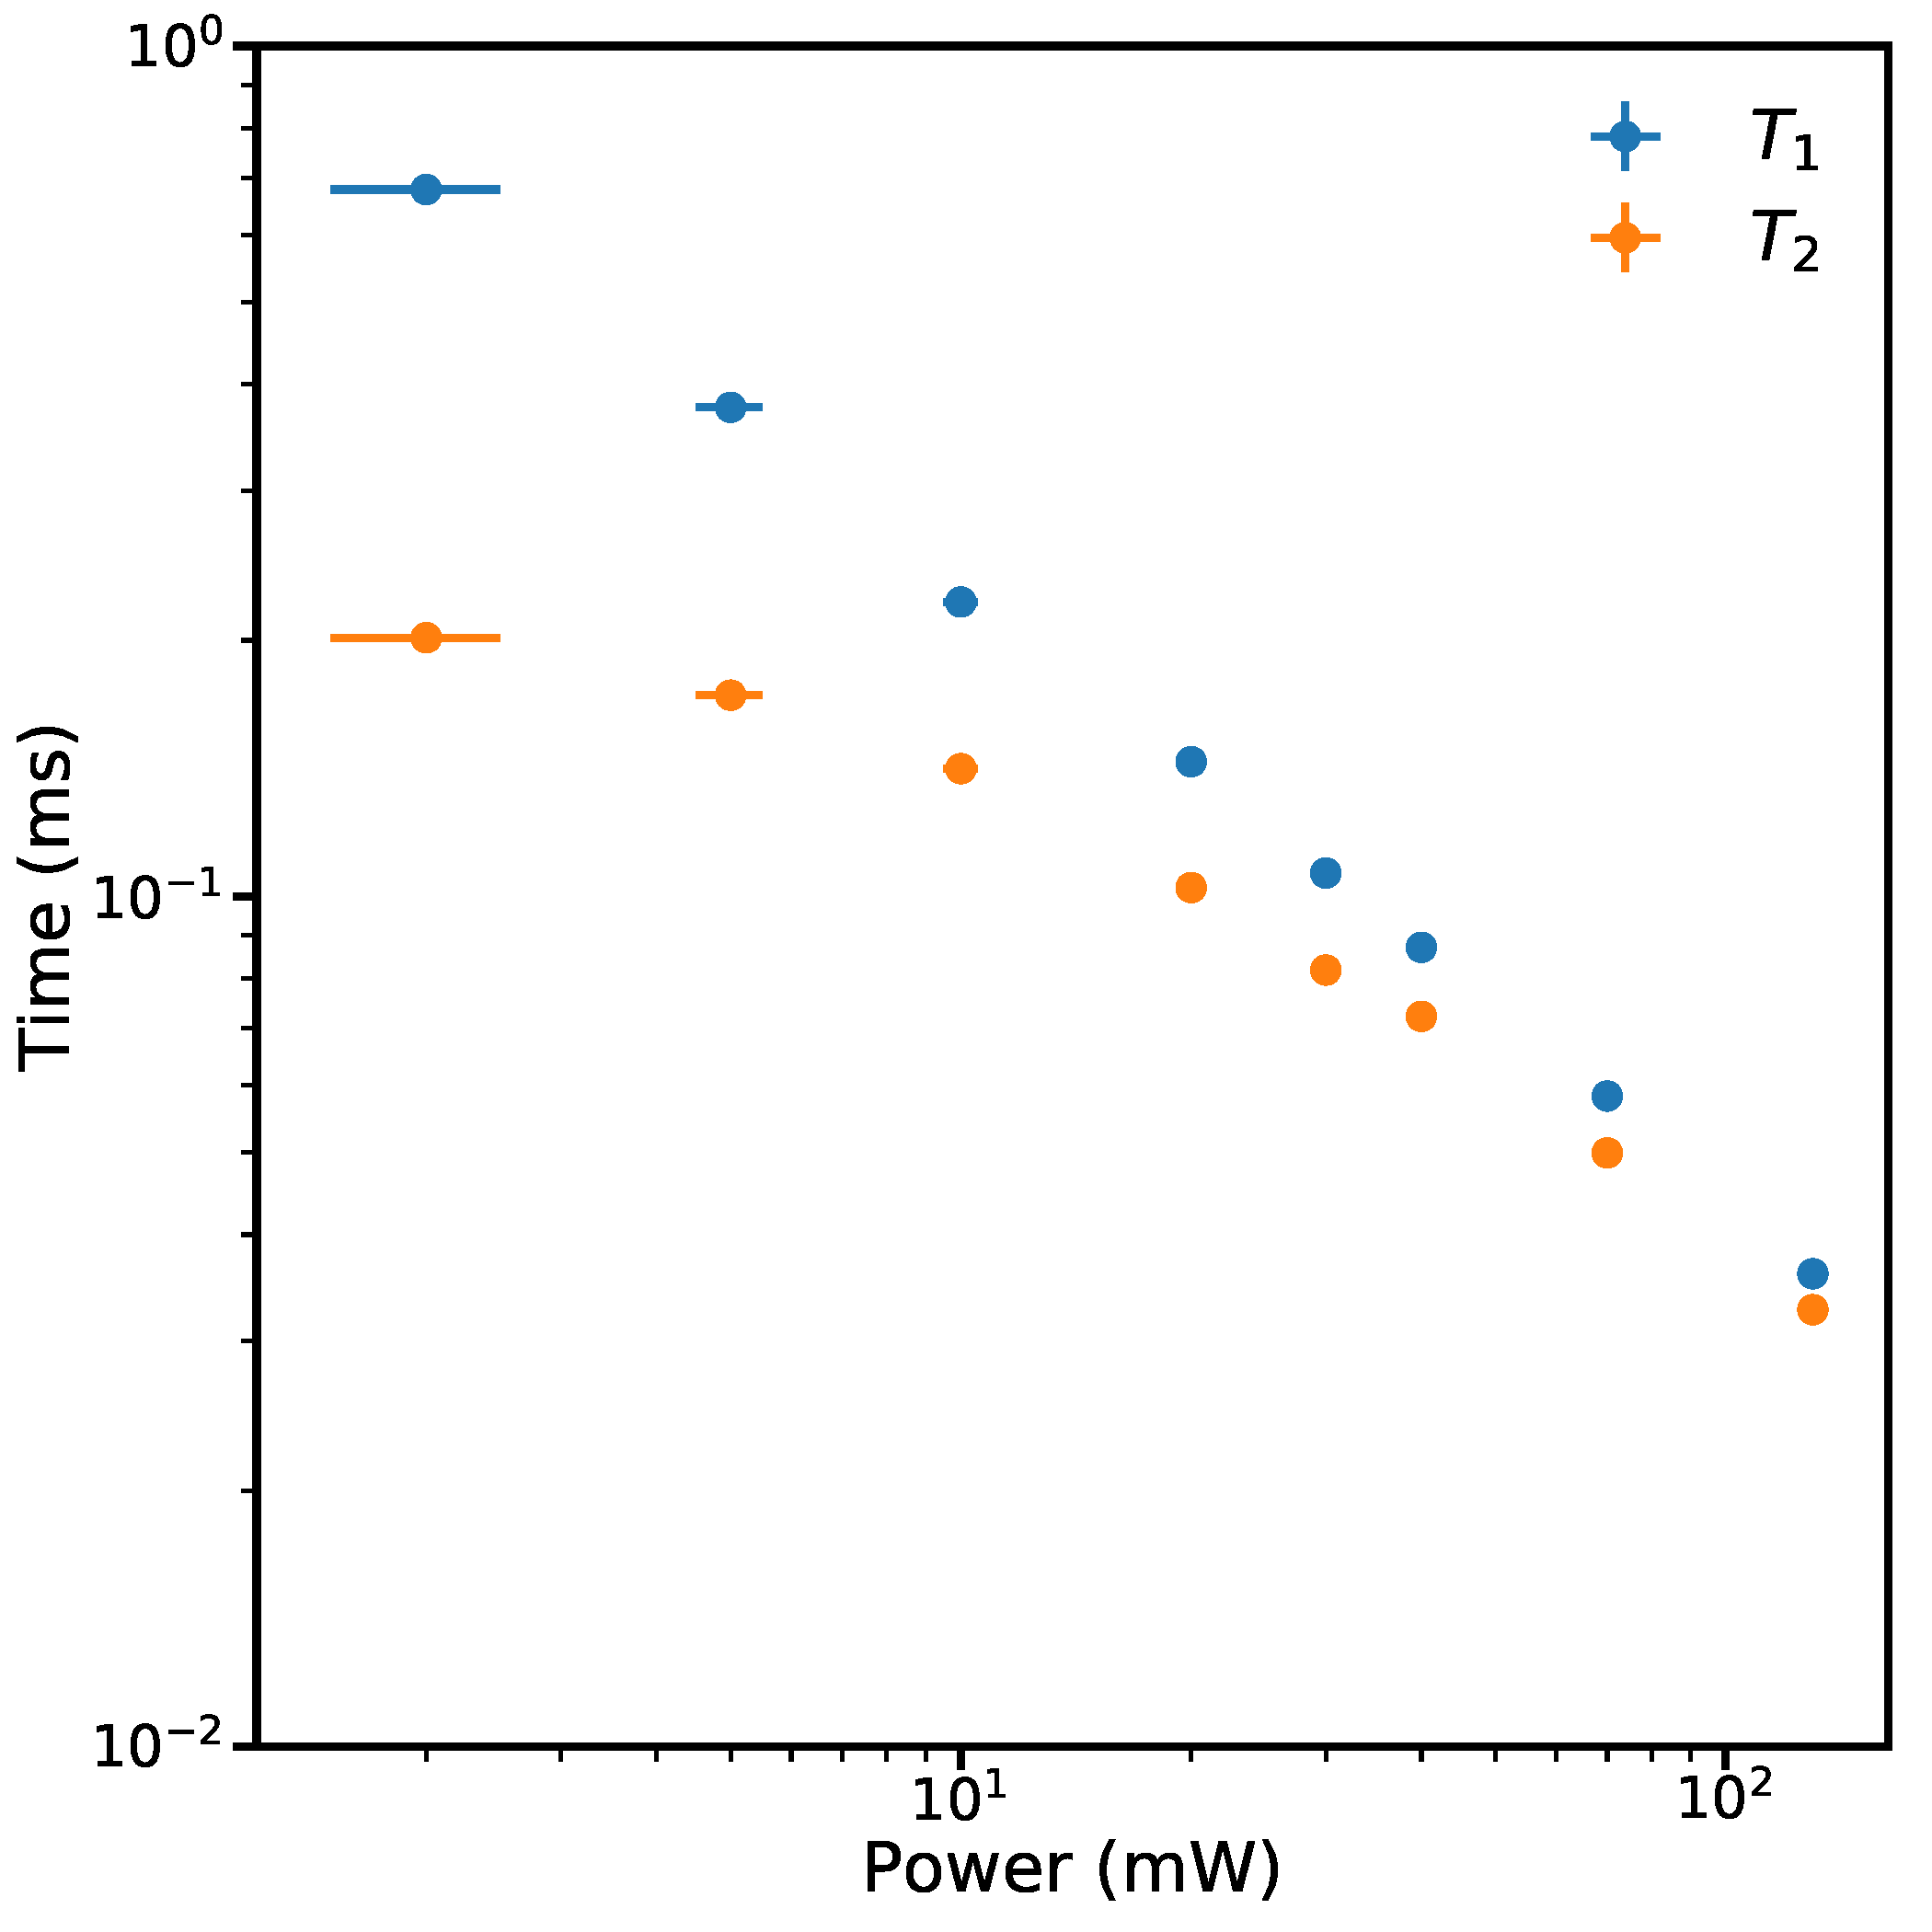
\includegraphics[width=\columnwidth]{Figures/T1vsT11070.pdf}
\end{subfigure}%
\caption[$T_1$ vs $T_2$ for 1058~nm and 1070~nm]{Figures showing how both $T_1$ and $T_2$ vary with laser power, presented on the same scale for ease of comparison. At high powers $T_1$ is observed to be close to $T_2$, essentially limiting it. }
\label{fig:t1vst2wav}
\end{figure}

\begin{figure}
\centering
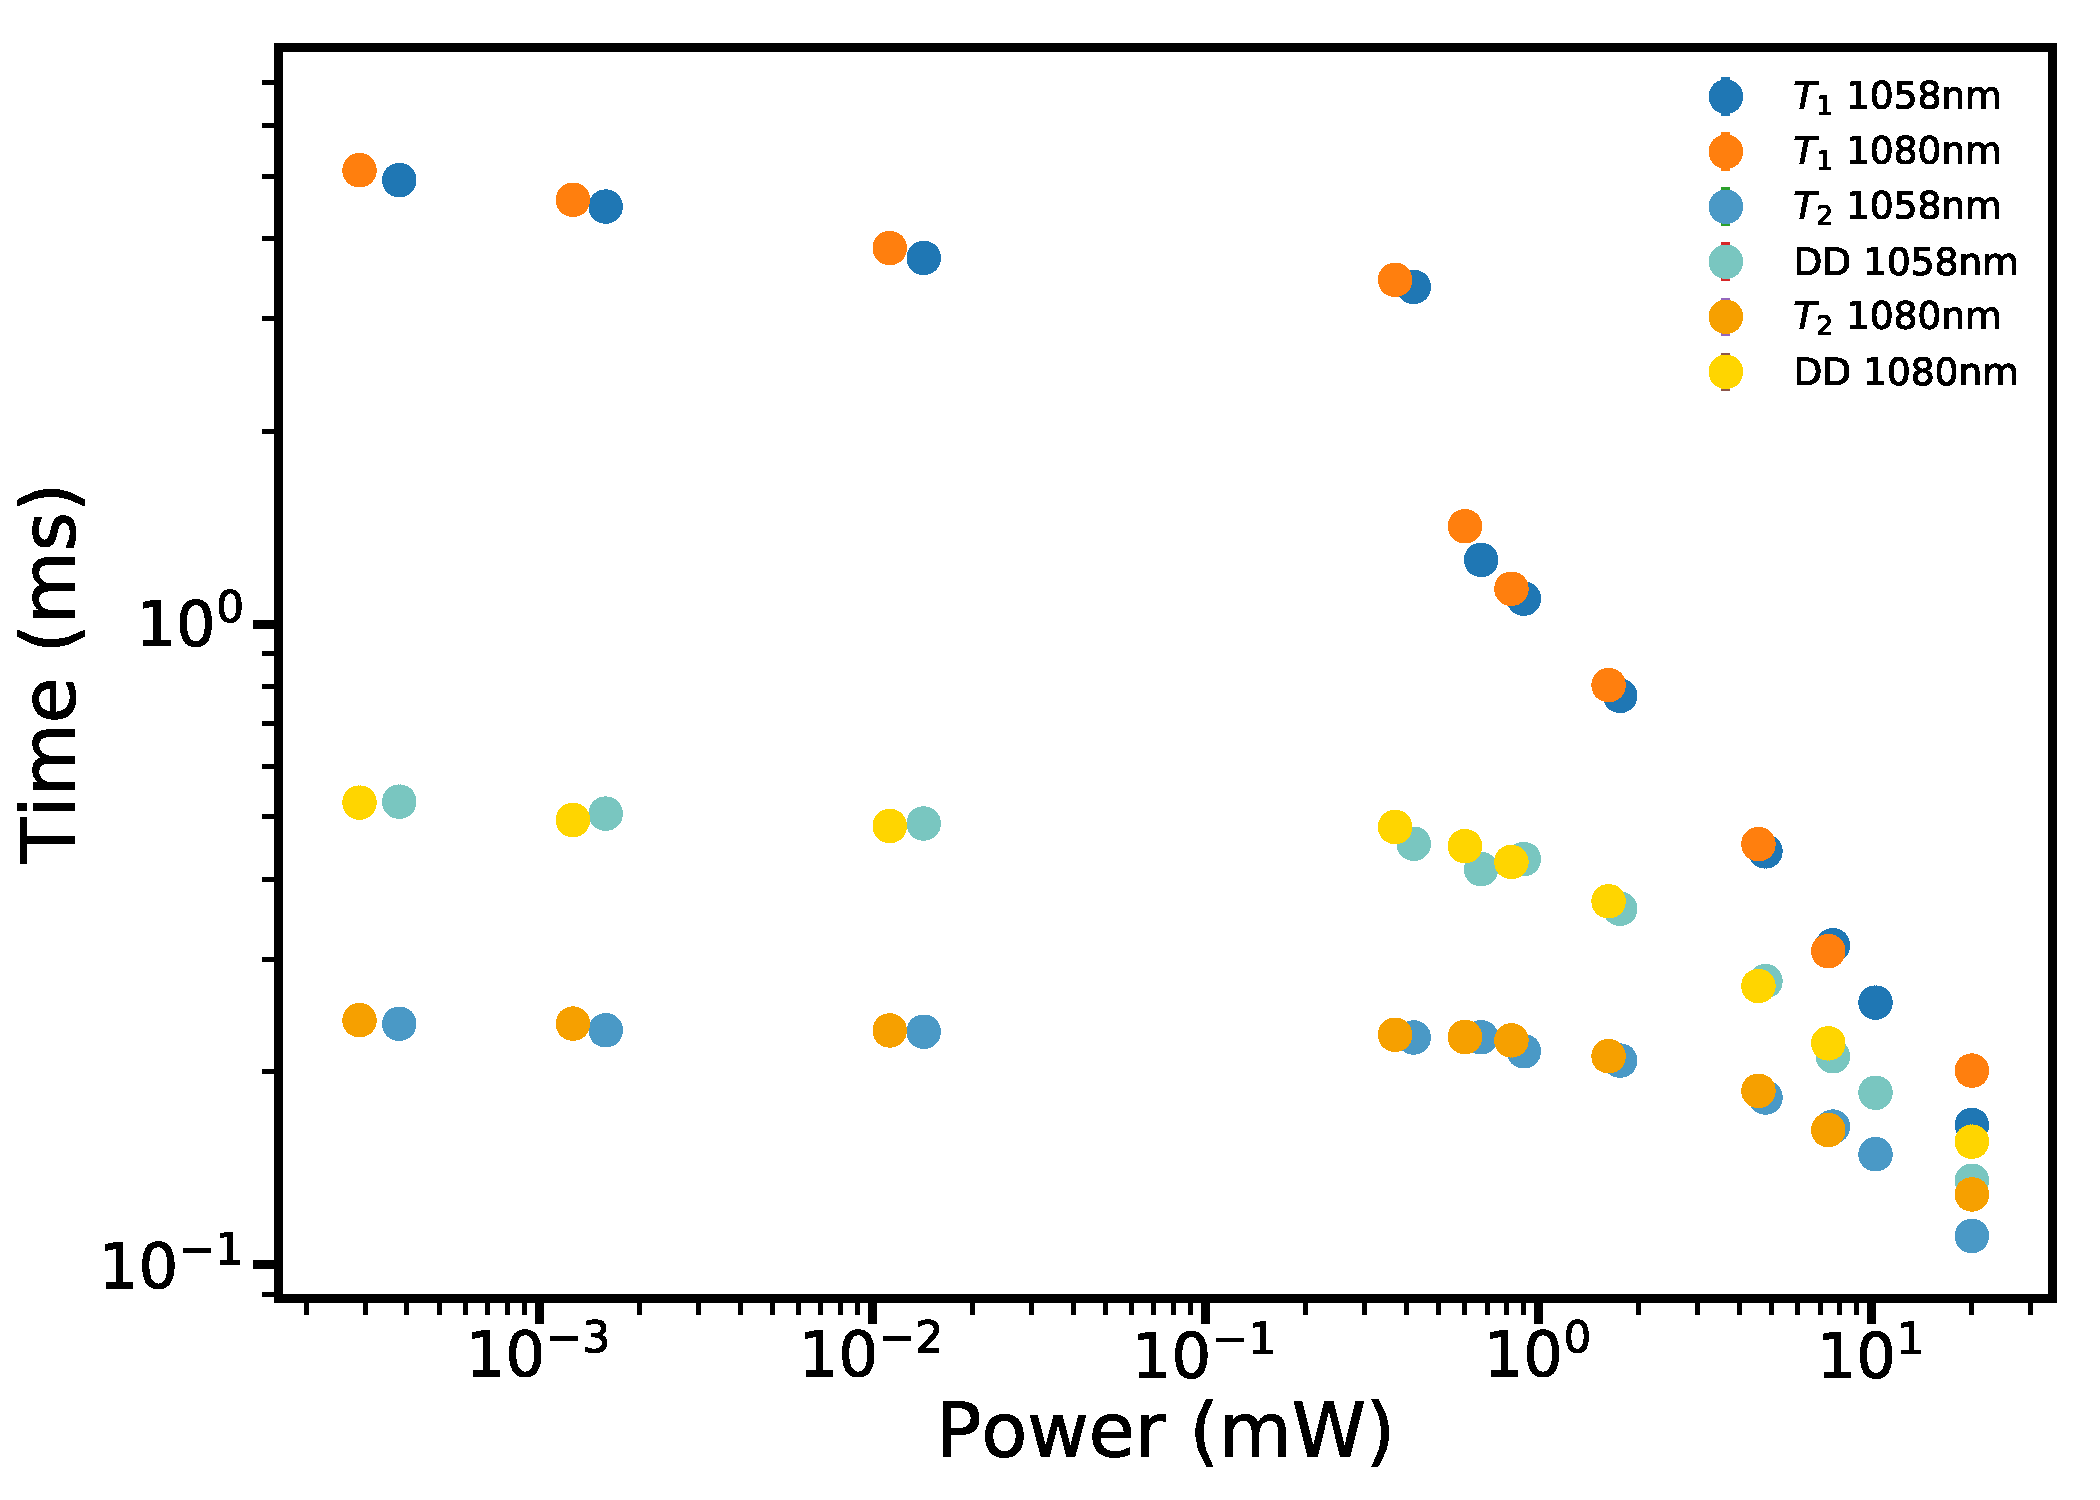
\includegraphics[width=0.8\columnwidth]{Figures/T1vsT2vsDD1058and1080.pdf}
\caption[Low power $T_1$ and $T_2$ comparison]{Figure shows the impact of laser illumination at low power and at wavelengths of 1058~nm and 1080~nm. For reference $T_1$ and $T_2$ in the dark are shown as black dotted lines ($T_1$ is the longer time-scale). $T_1$ is observed to saturate at very low laser powers, as it becomes close to the $T_1$ in the dark. Included is the coherence time for a 4 $\pi$ pulse dynamical decoupling sequence. This shows the expected increase in decoherence time at lower powers and continues to have an advantage over a traditional Hahn echo sequence as both begin to be reduced. Small differences in power at equivalent data points are due to the transmission of ND filters varying slightly with wavelength.}
\label{fig:t1vst2lowpow}
\end{figure}
The next question to be answered is whether the $T_1$ time will demonstrate a similar saturation behaviour as laser power is reduced as is demonstrated by $T_2$.
To see this lower powers must be used, achieved as described in section \ref{sec:lasExps} through the use of ND filters.
The results are shown in figure \ref{fig:t1vst2lowpow}.
These demonstrate that the $T_1$ does indeed saturate towards the dark $T_1$ at very low powers.
Of interest is the behaviour of the $T_2$ time as the $T_1$ time starts to be reduced significantly.
The $T_2$ time clearly starts to decrease \textit{before} it is strictly limited by $T_1$.
Several factors could explain this.
The first possibility is that the creation of free carriers promoted from the valence band is causing extra magnetic field noise at donor sites, reducing their $T_2$ time.
The difficulty with this particular mechanism is that there appears to be very little difference, at these low powers, between the $T_2$ times at the different wavelengths. 
Were this to be a significant effect then one would anticipate that it would be noticeably stronger in the lower wavelength case.
The alternative factors are $T_1$ related, were discussed in section \ref{sec:mechrelax}, and account well for the observed behaviour.
As relaxation rate increases, decoherence rate is also observed to increase before being strictly limited by the relaxation rate.
This is due in the main to the additional spectral diffusion processes as a result of neighbouring donor electron spin flips. 
As seen in figure \ref{fig:t1vst2lowpow}, dynamical decoupling gives an advantage over a Hahn echo sequence for decoherence time. 
As this is a natural silicon sample the advantage in the dark is to be expected, a small advantage remains even when the dynamical decoupling $T_2$ is shorter than the Hahn echo.
This suggests that the 4 pulse echo sequence is providing some protection from the mechanisms causing the increased decoherence rate - likely the spectral diffusion processes associated with an increased relaxation rate.
\\
The results here allow one important conclusion - there do not seem to be significant decoherence effects caused by laser illumination beyond the impact of an increased relaxation rate.
This is an important as it demonstrates that laser based read-out of measurement qubits is possible without destroying the quantum information held in data qubits, as long as power is sufficiently low.
To explore whether the impact on relaxation rates at a given laser power can be reduced I turn now to examine results at a lower temperature - 7k.

\subsection{Temperature Comparison}

A temperature comparison is useful primarily to give insight into the mechanism of increased relaxation rate.
A first expectation is that relaxation rate will begin to saturate at lower laser powers at lower temperatures, in line with the longer dark relaxation rate.
Particularly revealing will be a direct comparison between relaxation rates at the same wavelength and power, but at different temperatures.
If these are the same then it would suggest that whatever mechanism affecting the relaxation rate is temperature independent - potentially ruling out heating as a cause.
Figure \ref{fig:t1tempcomp} shows how $T_1$ changes with laser power at 1058~nm and at 7~K and 8k, with $T_1$s in the dark of 2.77~ms and 32.2~ms respectively.

\begin{figure}
\centering
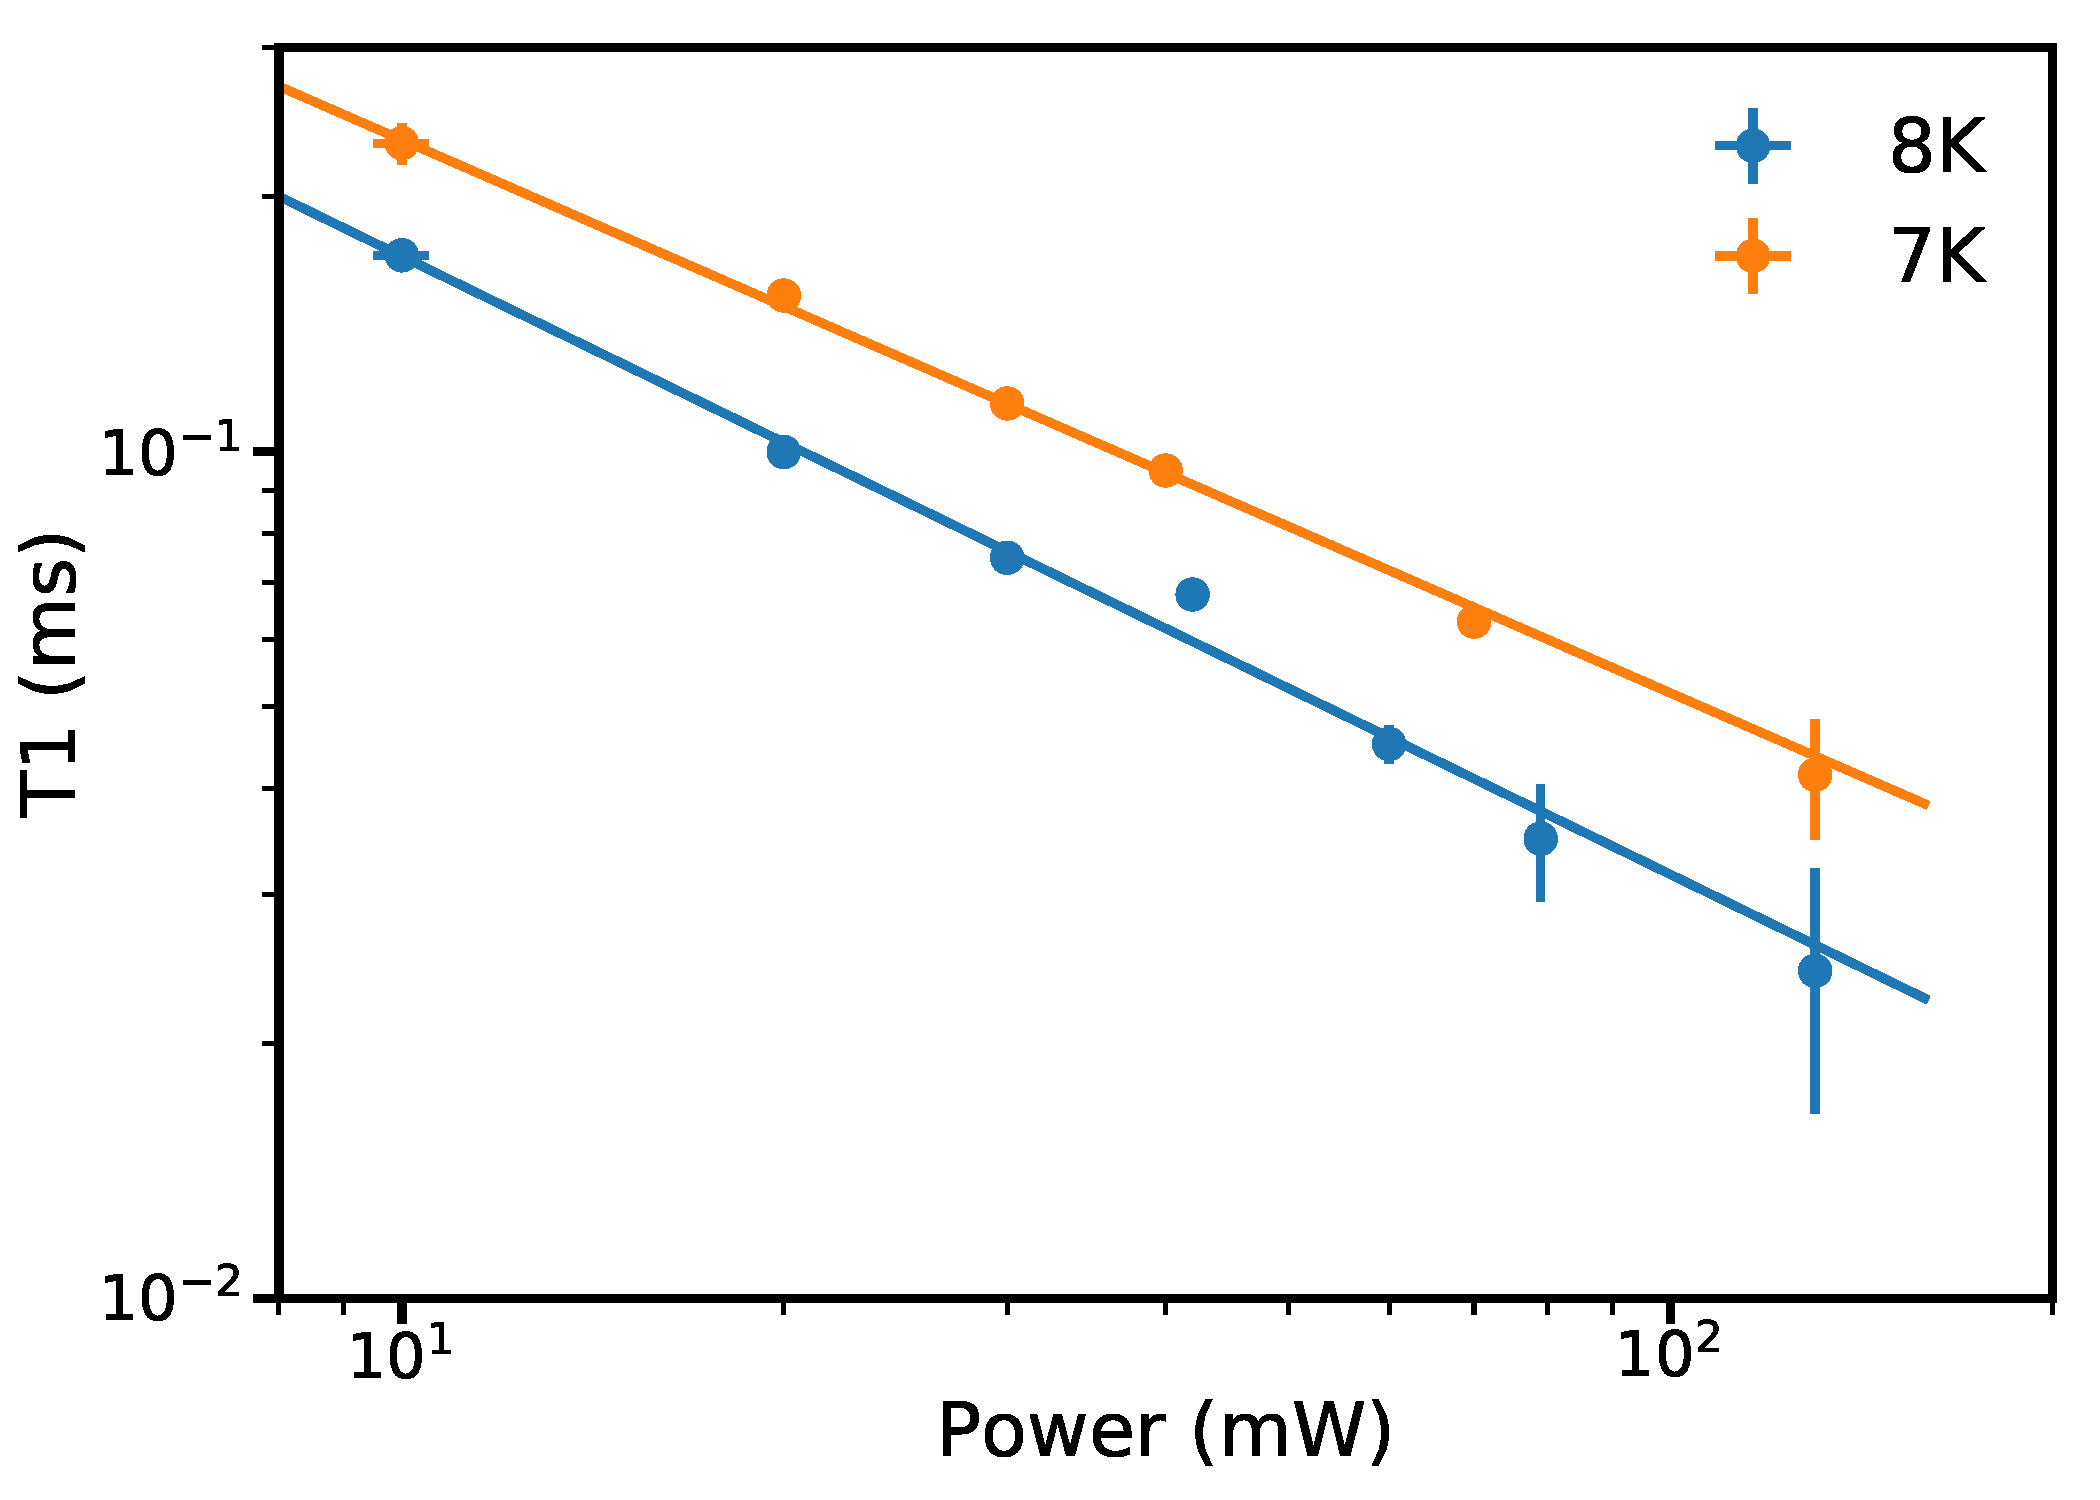
\includegraphics[width=0.8\columnwidth]{Figures/T17Kvs8k_1058nmTest.pdf}
\caption[$T_1$ temperature comparison]{Figure shows how $T_1$ changes with laser power at 1058~nm and for 8~K and 7~k, with respective dark $T_1$s of 2.77~ms and 32.2~ms. It is interesting to note that there is a clear increase in relaxation rate at 8~K vs 7~k. This suggests that the mechanism by which the laser acts has some temperature dependence.}
\label{fig:t1tempcomp}
\end{figure}

What is immediately clear from this comparison is that the laser is not a completely limiting factor - at the same power and wavelength but different temperatures different $T_1$ times are observed.
The 8~K fit has the same parameters as given above, whilst the 7~K fit has a power of $0.65\pm 0.002$.
At 7~K there is a clear increase in $T_1$ at the same laser power relative to 8k, suggesting that whatever mechanism is reducing relaxation time does indeed have a temperature dependence.
I will now address the mechanisms that are potentially responsible for the observed effects, concentrating on heating.

\subsection{Heating as a Mechanism of Relaxation}

Estimating the potential effect of heating as a result of laser illumination is complex.
The first factor affecting such an estimation is that the temperature sensor that is used to control the cryostat is not located on the sample so the highly localised heating caused by a laser would likely not be detected.
Beyond this, estimations are made difficult by the somewhat scarce information on light absorption at cryogenic temperatures in silicon.
The reason that heating is presented as a potential explanation for the observed relaxation effects is the extremely low heat capacity of silicon at cryogenic temperatures, as predicted by the Debye model \cite{ANDP:ANDP19123441404}.
This means that only a small amount of energy is required to effect significant heating in silicon.
Also relevant is that silicon is a poor photo-emitter, meaning that any infra-red radiation absorbed is likely to end up as heat rather than emitted photons. 
Calculating potential heat rises is made difficult by the scarcity of literature on the absorption coefficient of silicon at low temperatures.
Studies have concentrated on silicon at room temperature due to its use in solar cells and have tended to assume that low-temperature, below band-gap absorption will be low due to the scarcity of phonons to assist transitions and conduction band electrons to absorb sub band gap photons.
Interest has been peaked recently due to the possibility of taking advantage of the anticipated high transmission qualities of silicon at low temperatures for use as an interferometer in a gravitational wave detector \cite{Degallaix2014}.
One study in particular provides a useful insight, although not a directly comparable one.
This measured the absorbance of silicon at 6~K by monitoring its temperature increase under illumination by a 1550~nm laser.
Results of this experiment show a much greater absorption than anticipated, with the measured result being the same at 6~K as at room temperature: 0.030cm$^{-1}$.
Taking this figure as a guideline, it can be estimated that approximately $0.5\%$ of incident light is absorbed by the sample in these experiments.
Harder to estimate is the rate at which the sample is cooled in the cryostat, which will determine how much extra energy it holds in equilibrium with the laser turned on.
In \cite{Degallaix2014} the sample was observed to increase in temperature as long as the laser was turned on.
It was, however, poorly thermally coupled to its cooling environment and it seems likely that a sample in direct contact with helium flow will reach an equilibrium temperature value.
Here I make the assumption that approximately $1\%$ of the laser power is retained in the sample at equilibrium, adding to its temperature.
This figure can then be used along with heat capacity, taken from \cite{Desai1986,Glazov2001}, to calculate the expected temperature for a given laser power.
Using this temperature along with the equations in section \ref{sec:mechrelax} allows an estimation of $T_1$ and $T_2$ times at given laser powers.
\\
A further potential contributor to relaxation rates is donor ionisation - unpaired electrons on the donor being excited to the conduction band by an incident photon.
This would be registered first as a loss in signal and then a relaxation back to thermal equilibrium as the donor is recaptured by an ionised donor.
This process also contributes to heating of the sample - an electron excited to the conduction band \emph{thermalises} (relaxes to the energy minimum of the conduction band) rapidly - but this effect is already accounted for in the heating calculation.
The cross section for this process is predicted to be small - peaking at $17\times10^{-16}\text{cm}^{-2}$ and significantly smaller at the wavelengths used in these experiments \cite{Sclar1984,Ross2017a}. 
Following \cite{Ross2017a}, a figure of $1.5\times10^{-16}\text{cm}^{-2}$ is used to calculate rate of donor ionisation with power.
Given these parameters, a simulation of relaxation rate based on laser power, when accounting for donor ionisation rates and heating effects is given in figure \ref{fig:t1t2sim}.

\begin{figure}
\centering
\begin{subfigure}[b]{\textwidth}
\centering
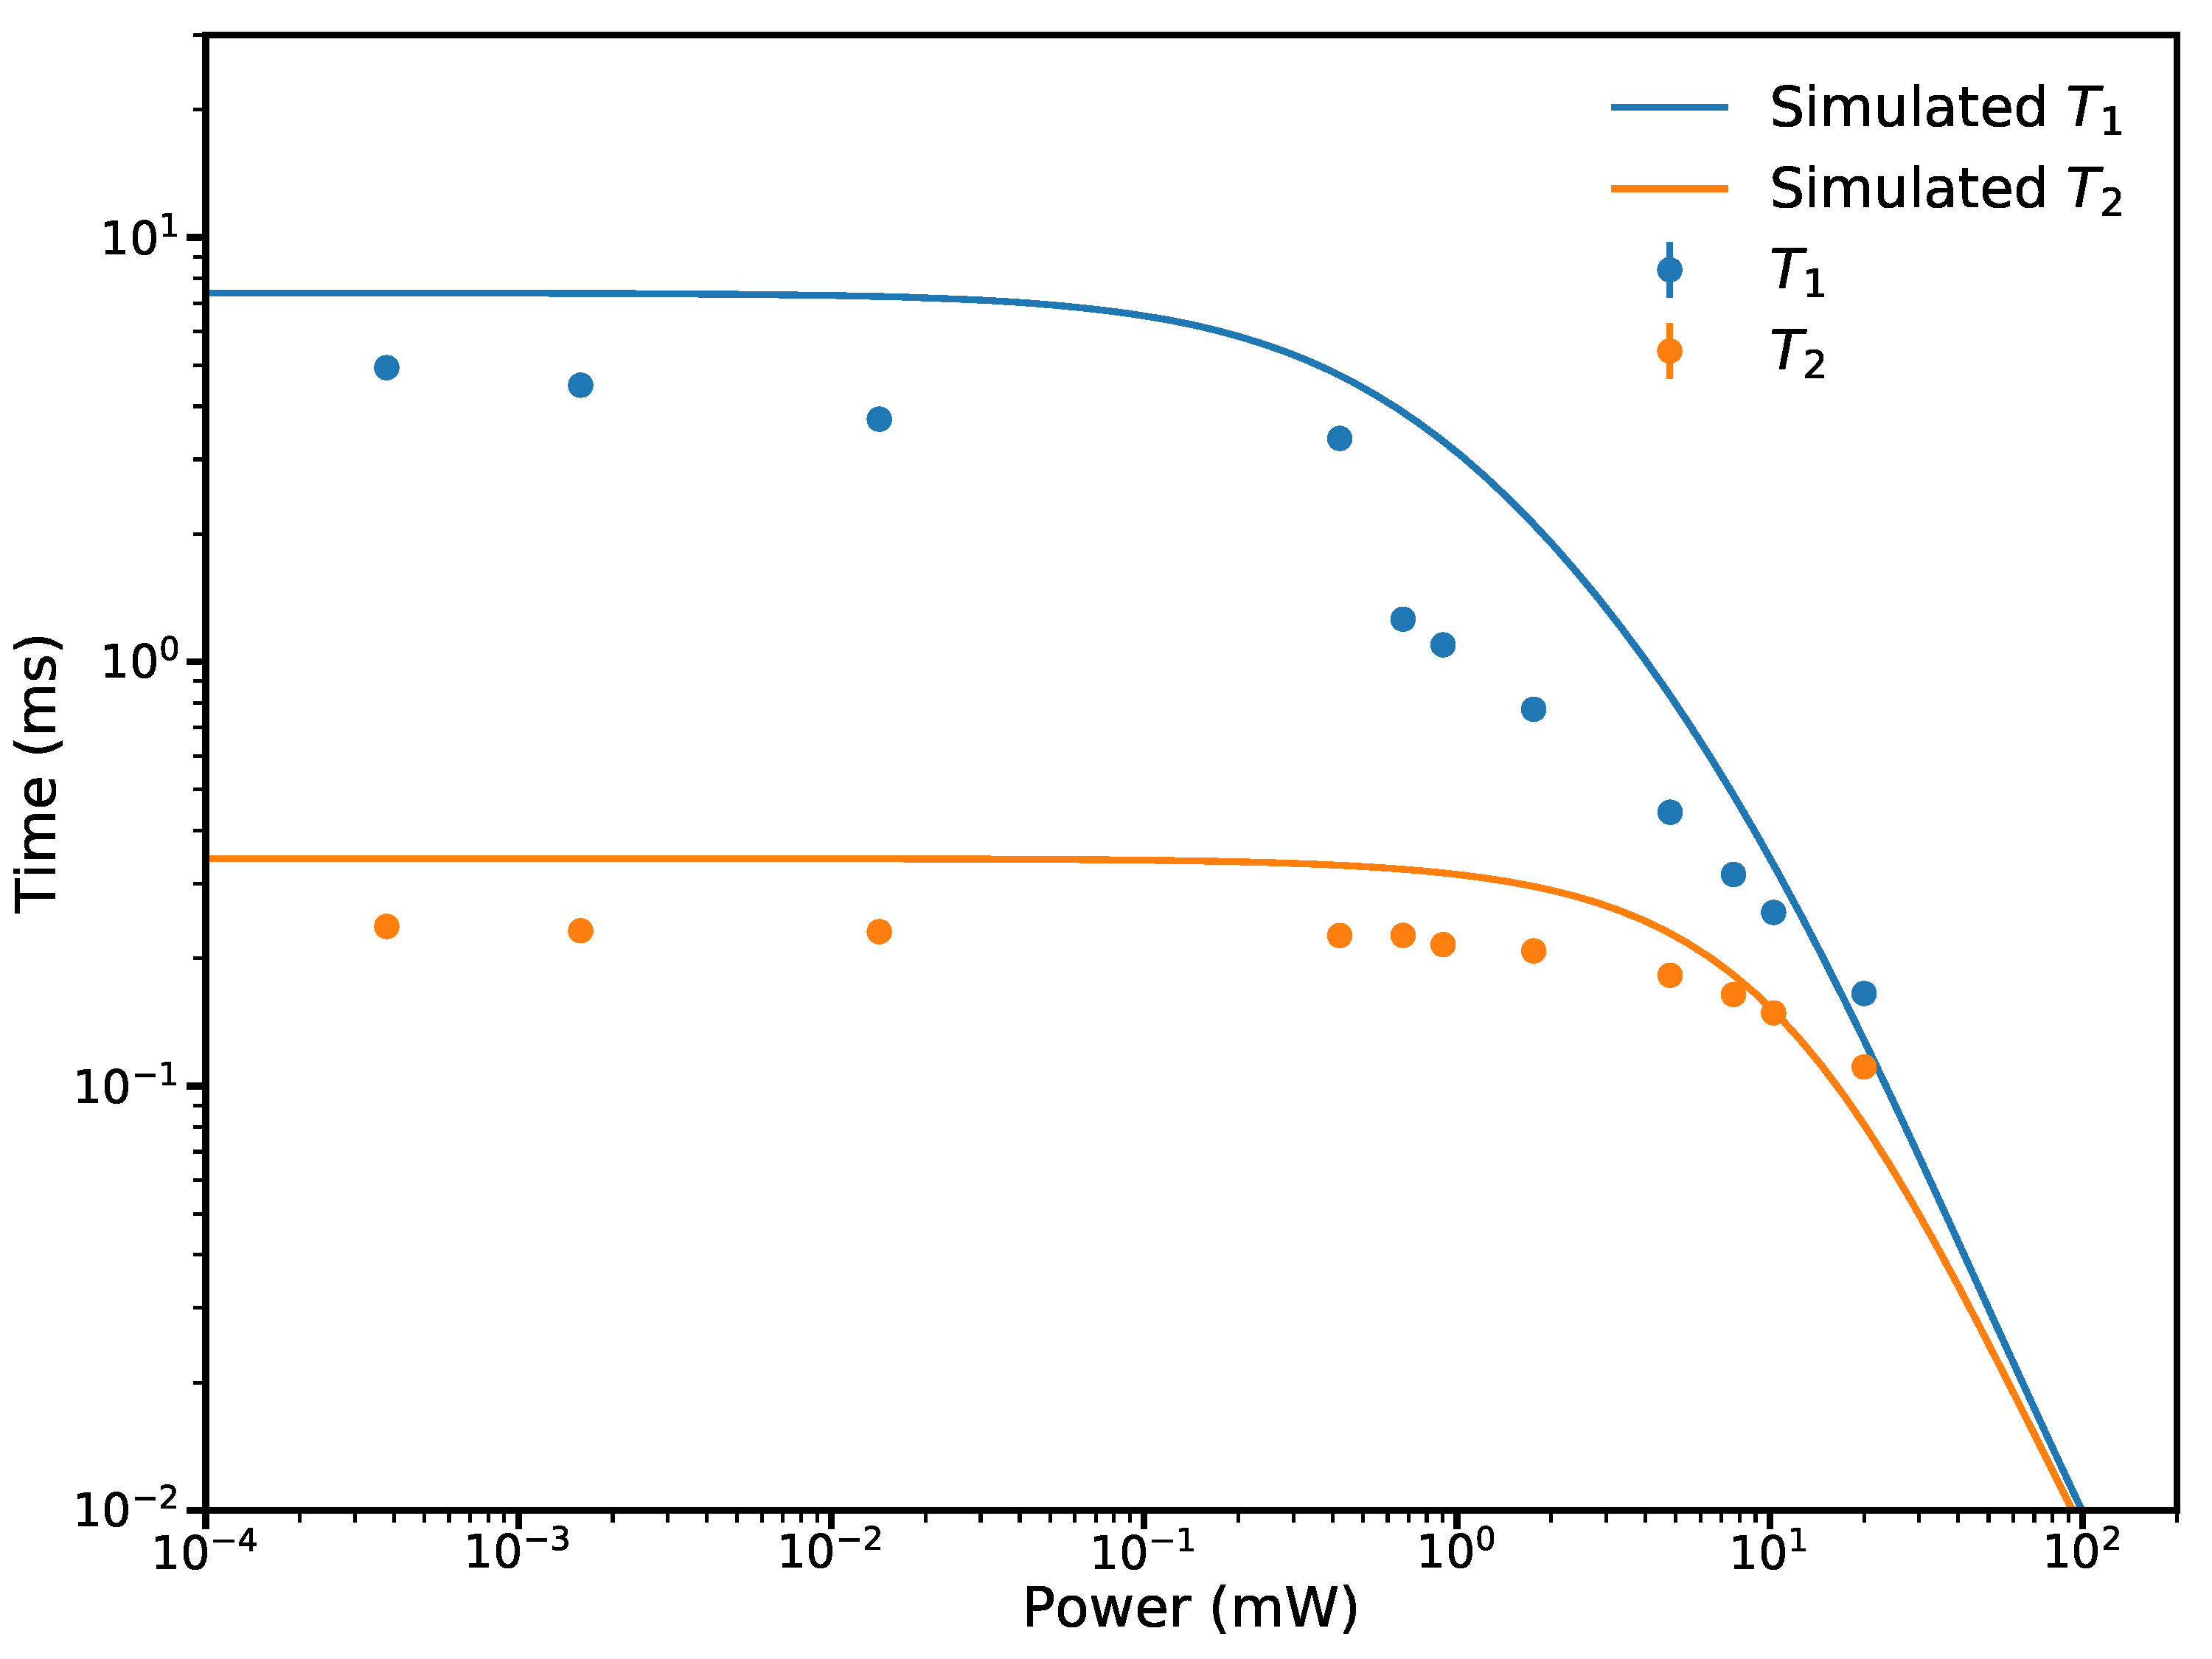
\includegraphics[width = 0.8\columnwidth]{Figures/simt1t2.pdf}{(a)}
\end{subfigure}
\begin{subfigure}[b]{\textwidth}
\centering
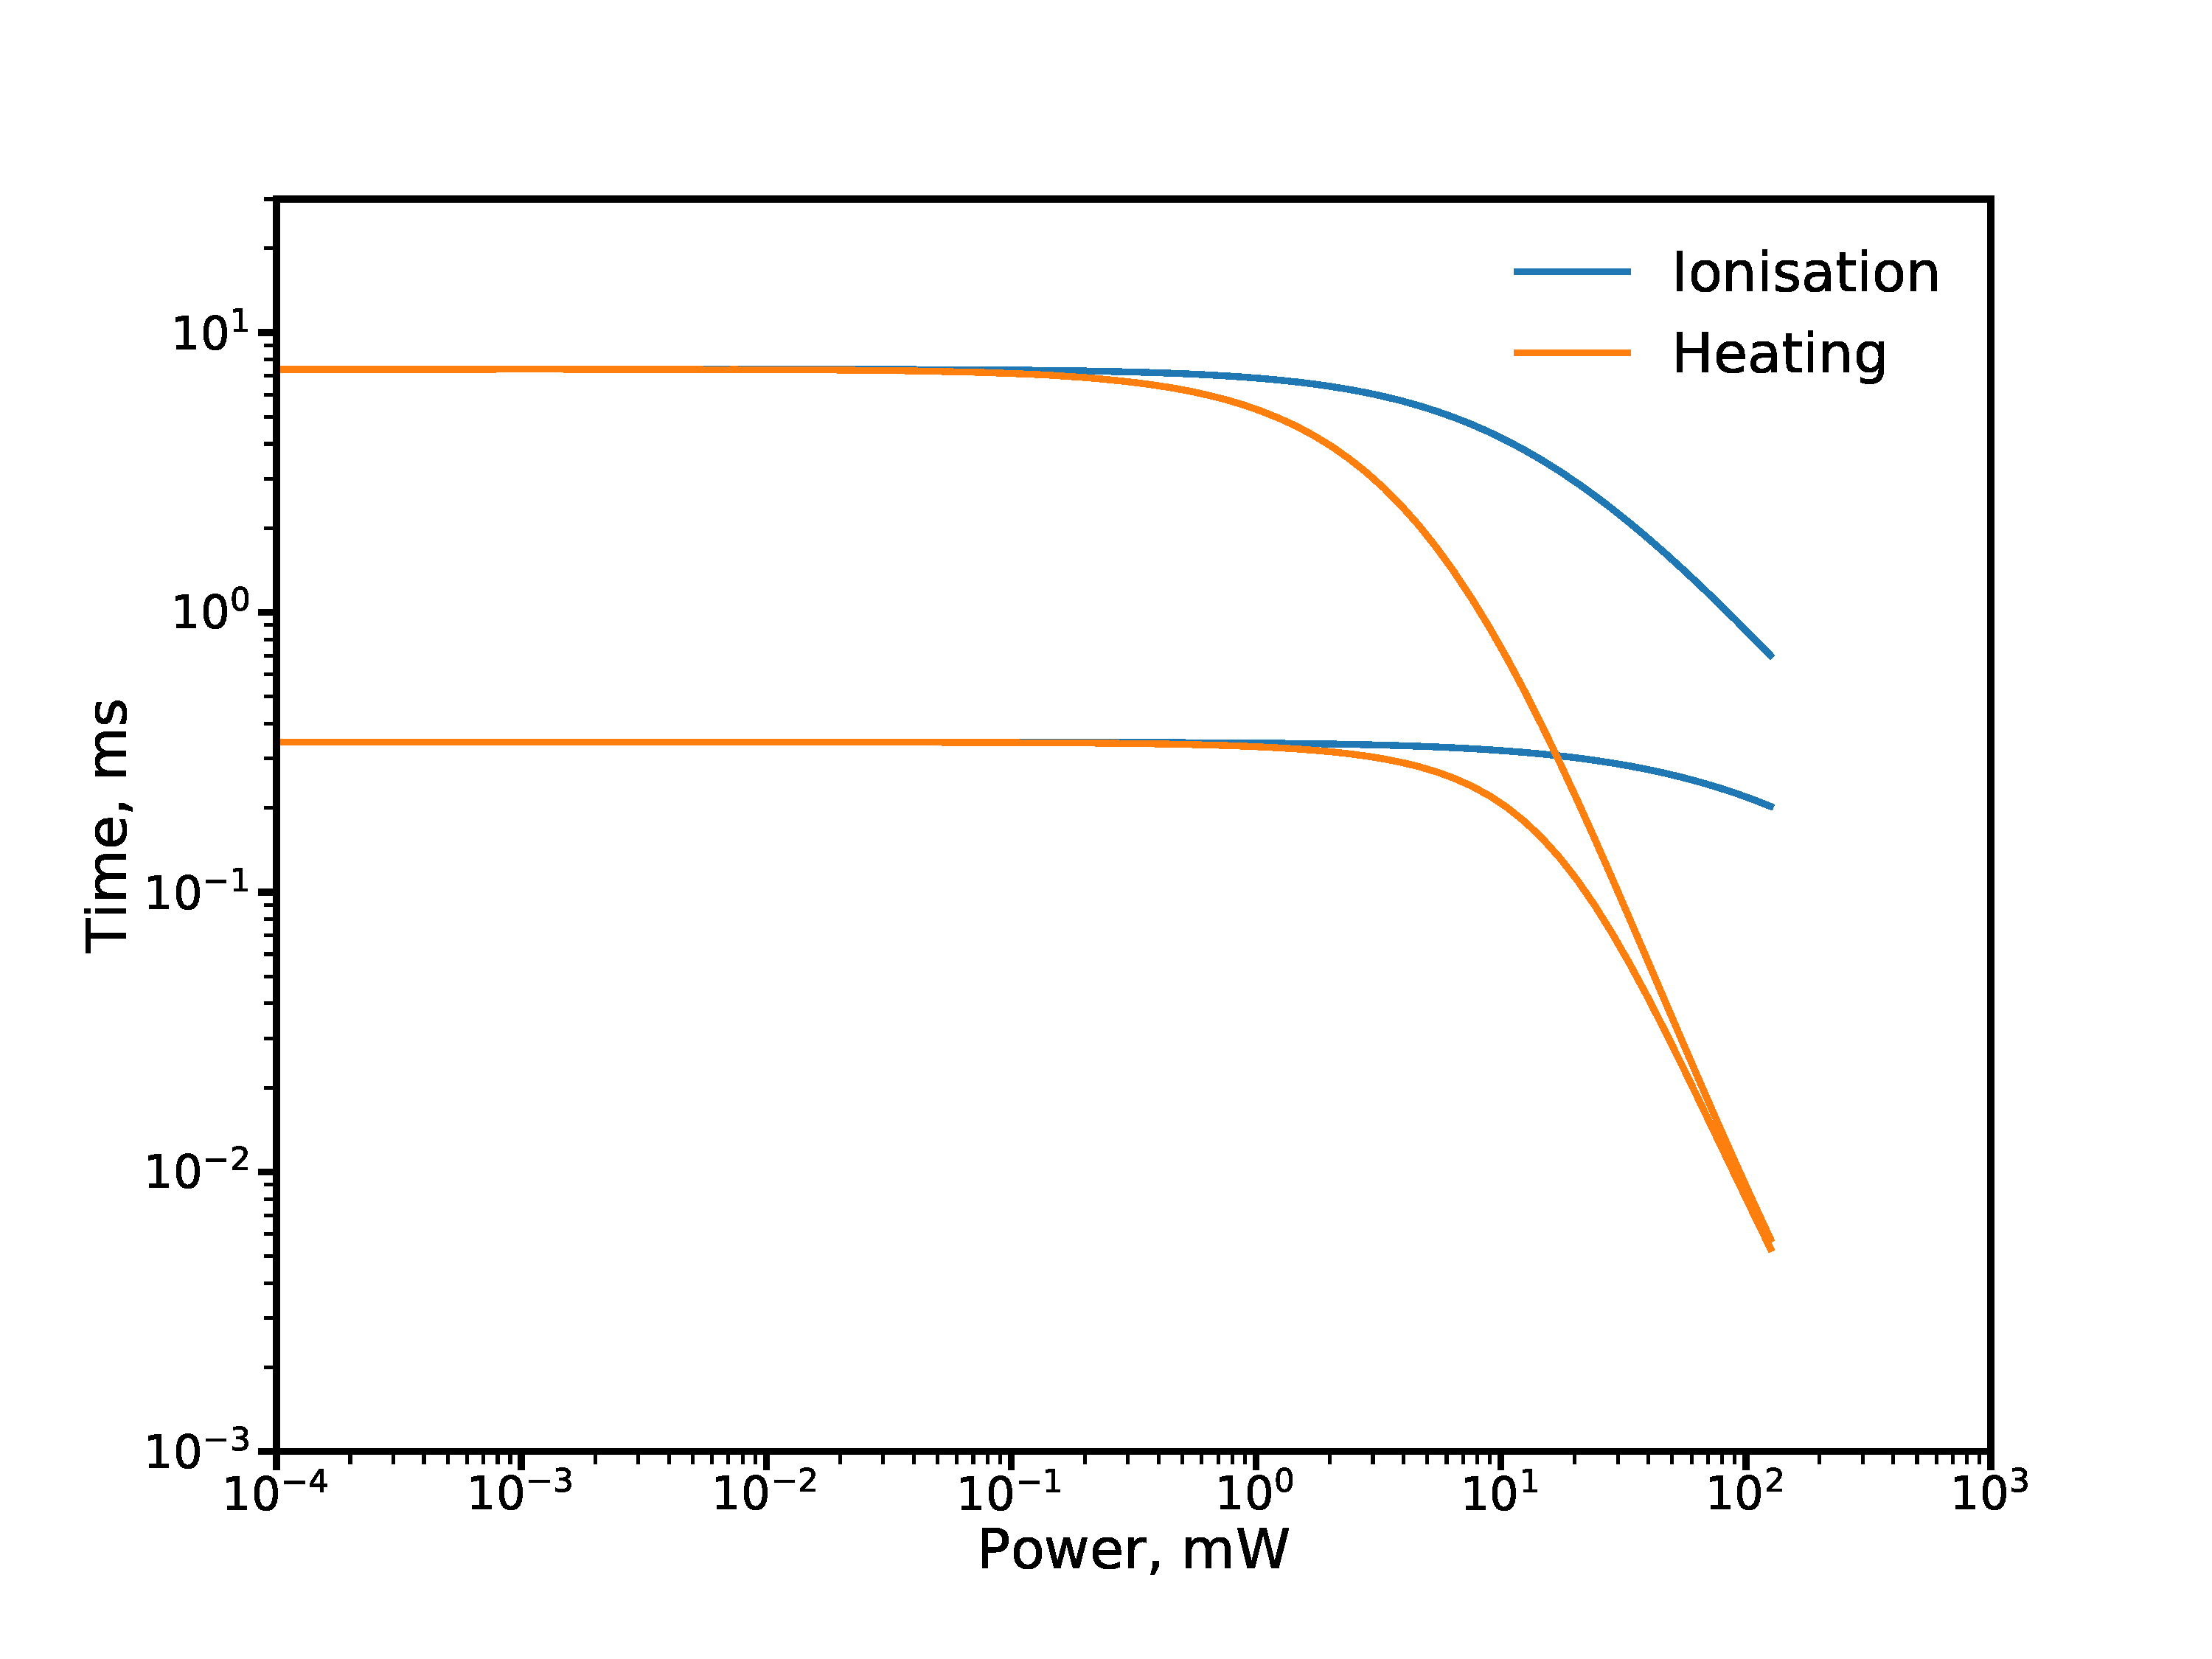
\includegraphics[width = 0.8\columnwidth]{Figures/ionvsheat.pdf}{(b)}
\end{subfigure}
\caption[Simulated $T_1$ under heating]{Figure showing the simulated $T_1$ and $T_2$ as as a function of laser power at 8~K when taking account of potential heating and donor ionisation, alongside low power data taken at the same temperature. \textbf{(a)} shows the combined impact of heating and donor ionisation whilst \textbf{(b)} shows their individual contributions - demonstrating that heating is the apparently dominant effect. Data for $T_1$ and $T_2$ calculated using heat capacity of silicon at these temperatures alongside equations shown in section \ref{sec:mechrelax}, whilst donor ionisation rates use cross sections given in \cite{Sclar1984,Ross2017a}.}
\label{fig:t1t2sim}
\end{figure}

The results shown here, whilst by no means conclusive, suggest that heating is a potential cause of the observed effects.
Some wavelength dependence would also be expected with a heating based mechanism - as the absorbance of the laser light is dependent upon the wavelength. 
At higher powers the heating effect appears to increase faster in the simulation than in the experimental results but further work will be required to refine these figures.
Heating does appear to account quite well for the observed discrepancy in $T_1$ and $T_2$ times at each temperature.
\\
I have not discussed the mechanism that Feher and Gere identify as the most prominent in their results: the double spin exchange between free electron, donor electron and donor nucleus.
This process, although mentioned by Feher and Gere, is given no explicit form.
A qualitative argument is used to explain why it accounts for the observed behaviour of electron relaxation time under illumination.
As such it is difficult to incorporate such a mechanism into my simulations.
One question would be whether this mechanism would demonstrate the temperature dependence that has so far been observed, with relaxation occurring more slowly at lower temperatures but under the same illumination.
It is possible that the lower thermal velocity of free electrons at lower temperatures could account for the discrepancy, giving a smaller number of double scattering events per second.
This presents an excellent next step for this work: determining both the density of free carriers at each wavelength and using this to provide an account of the scattering rate of electrons on donors.

\section{Stark Shift Experiments}

\subsection{Stark Shift on Selenium Donors}

Observing the Stark shift proved challenging initially, with a replication of the previous experimental set-up not yielding the results that were expected when the set-up was tested on previously investigated systems.
This proved to be due to a flaw in the positioning of the plates used to produce an electric field relative to the sample.
Contact between the plates and the sample was required to observe a Stark shift.
Once the set-up issues had been established a Stark shift was observed in bismuth, replicating a prior experiment \cite{Wolfowicz2014}, as seen in figure \ref{fig:biStark}.


\begin{figure}
\centering
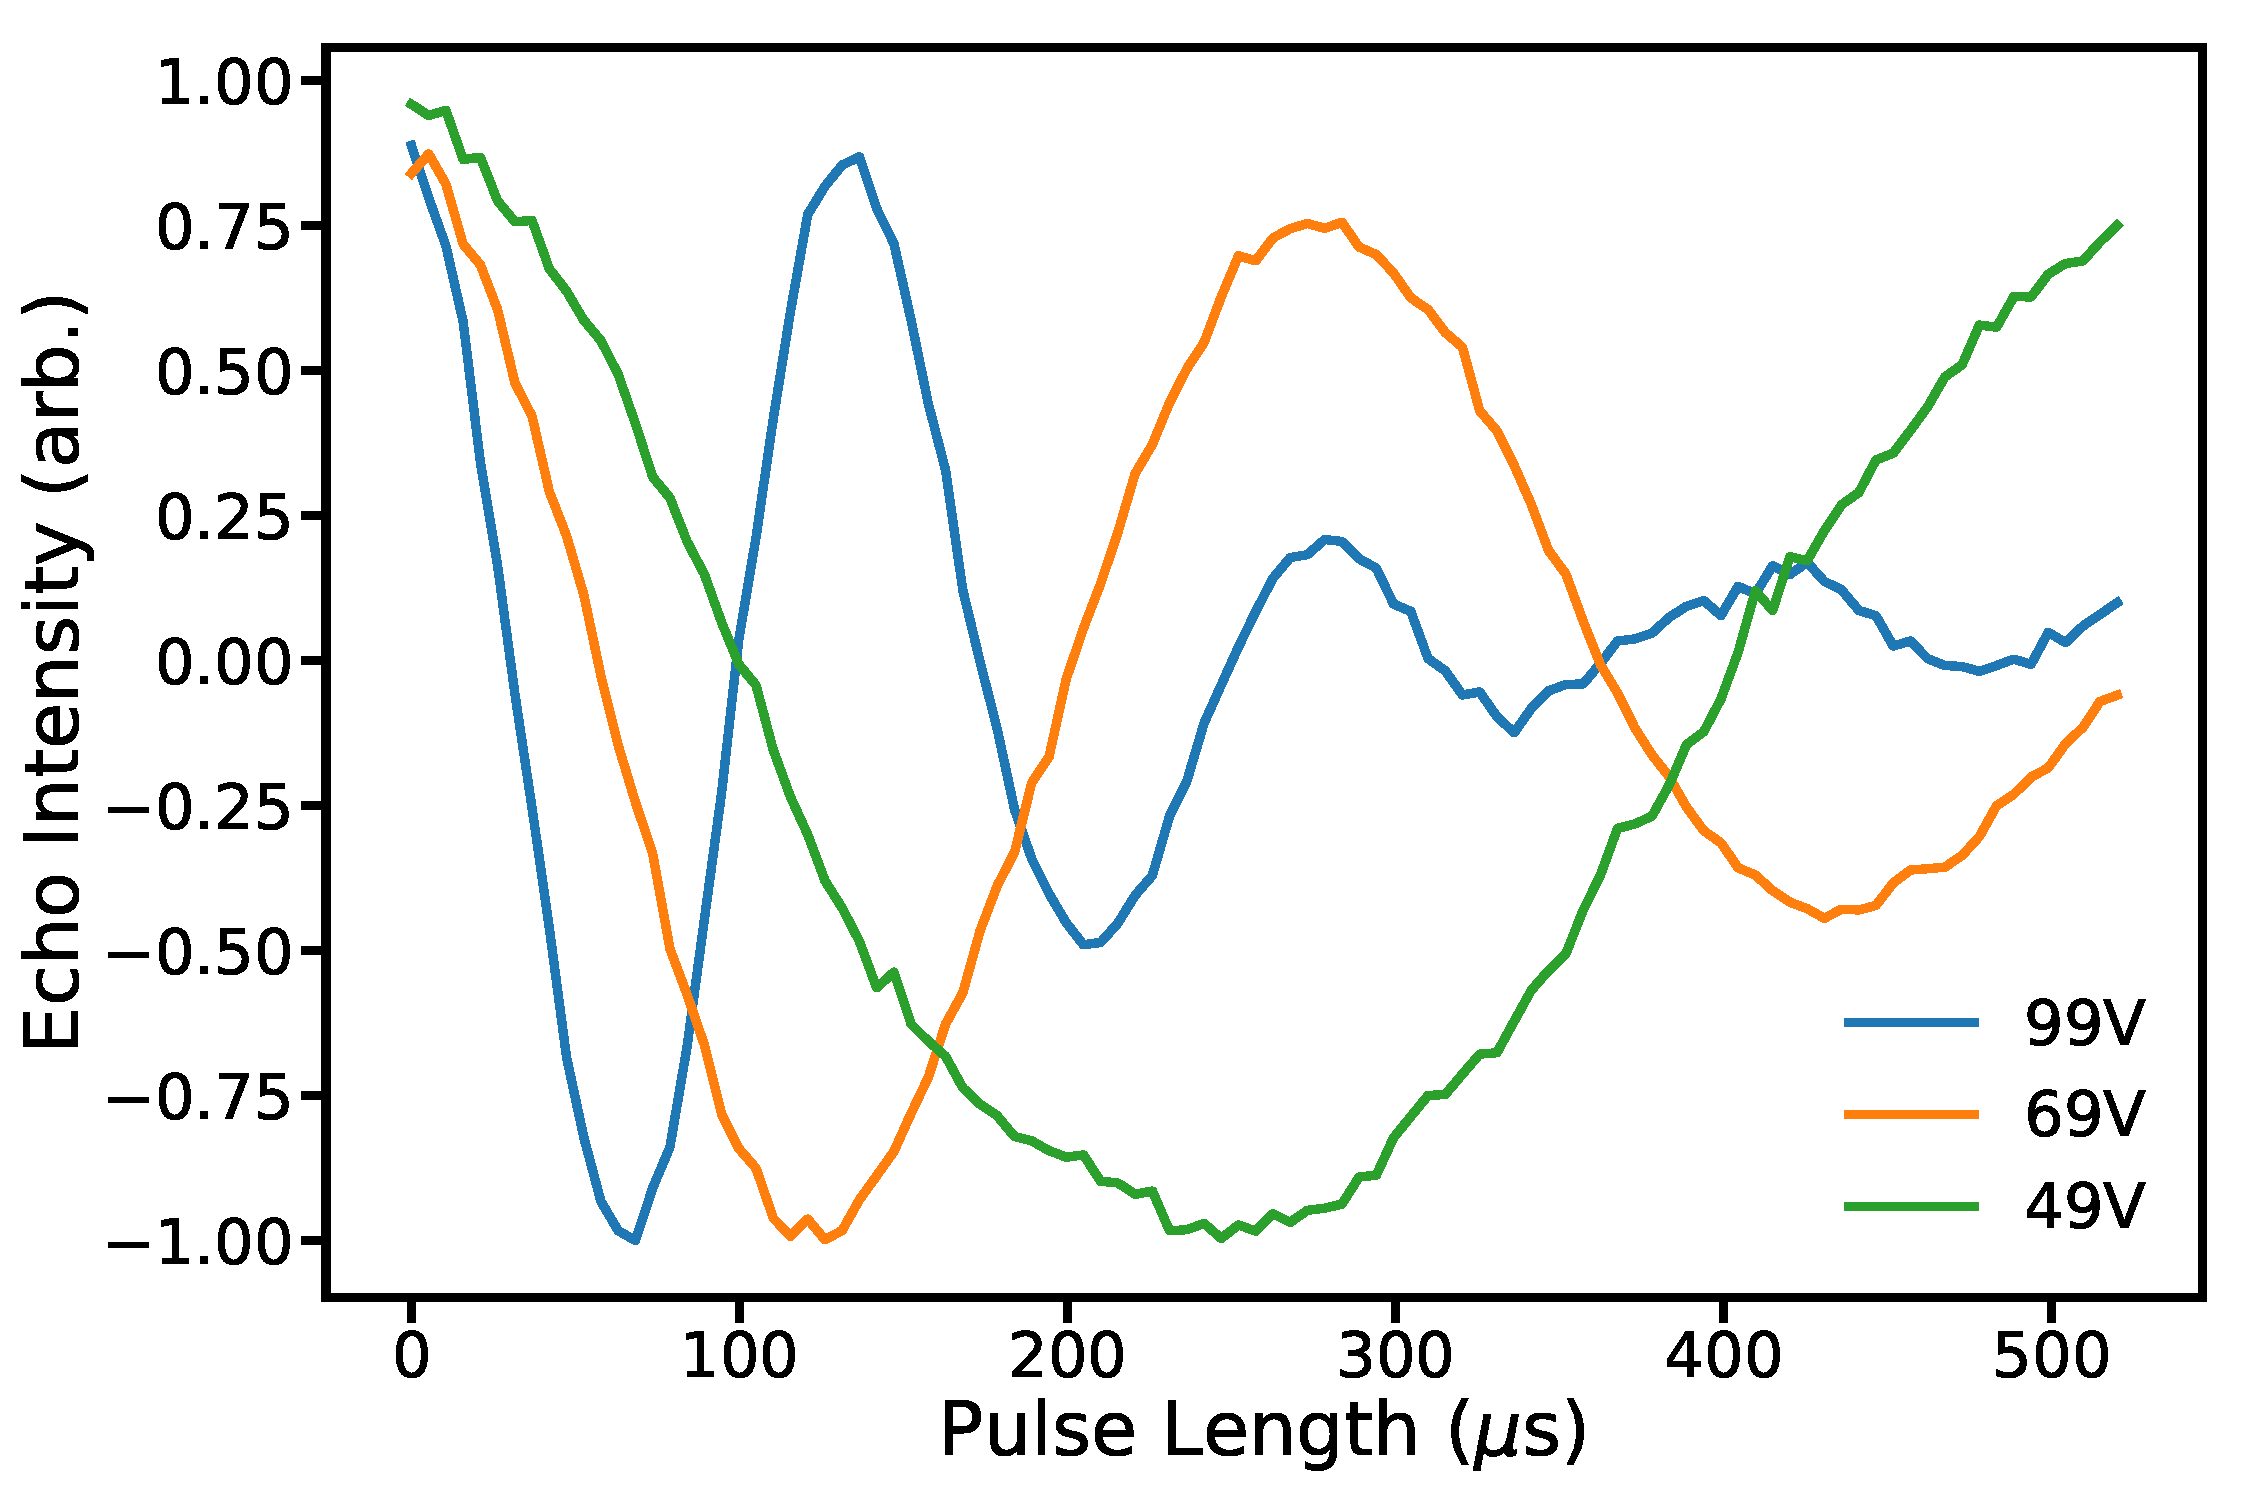
\includegraphics[width=0.8\columnwidth]{Figures/BiMultiVolt.pdf}
\caption[Stark shift in bismuth]{Figure showing the Stark shift in bismuth as a result of bi-polar voltage pulses applied in one half of a Hahn echo sequence causing a phase shift in the electron precession. Oscillations frequency is proportional to the square of the voltage applied. The decay in the signal as the pulse length increases is a result of the inhomogeneous linear Stark term causing the loss of phase coherence.}
\label{fig:biStark}
\end{figure}

This figure shows the oscillation in phase of the echo signal as the voltage pulse length is increased.
The oscillation is proportional to $E^2$, causing the increase in oscillation rate as voltage is increased.
The decay in the oscillations, particularly clear in the 99V case, is caused by the contribution of inhomogeneous linear electric field terms.
Although the impact of these terms is reduced through the use of bipolar pulses, their effect cannot be completely negated due to imperfect pulses and the imperfect plate geometry creating inhomogeneity. 
Strain is a strong contributor to this effect meaning that excessively firm contact between plates and sample results in the rapid decay of the signal.
\\
Difficulties have been encountered measuring the Stark shift on selenium, in part due to its expected low value.
As discussed in section \ref{sec:starkShiftLit}, the Stark shift is caused by a mixing between the ground state of the electron on the donor and higher energy levels leading to a modulation of the Hyperfine coupling between electron and nucleus.
The gap to first excited state in selenium (as a deep donor) is significantly larger than in the shallow donors in silicon. 
For example: phosphorus has a gap to the first excited state of $10.5$meV, bismuth $33.8$meV; selenium has a gap of $429$meV \cite{LoNardo2015,Nardo2015}. 
As yet no Stark shift has been observed in Selenium, using pulses of up to 800$\mu$s long at $\pm99$V.
By taking the maximum possible unobserved phase shift as being equal to the signal to noise ratio of the obtained data it is possible to obtain a value for $\eta_A$, the hyperfine Stark shift coefficient, of 0.7$\times10^{-7}$.
I am not yet fully confident in this result due to several issues with the current experiment.
The first of these is that it has been shown to be extremely sensitive to experimental set-up - strain and lack of contact between the plates and the sample rendering the results inaccurate.
The sample being used for these experiments is quite large, being 4mm $\times$ 4mm $\times$ 2mm.
This means that the plates cannot cover the entirety of the sample and remain able to fit in the spectrometer cavity.
The presence of selenium also means that electrons preferentially populate these impurities, rather than any phosphorus impurities in the sample.
This makes it hard to verify the Stark shift on a phosphorus transition before measuring a selenium transition.
One possible approach would be to populate the phosphors impurities by using an above band gap laser pulse - a technique used in the group previously \cite{Nardo2015}.
This would allow verification of the strength of the Stark shift on phosphorus prior to measuring it on selenium - allowing confidence in the experimental set-up.

\subsection{Stark Shift on $^{29}$Si Nuclei}

The final experiment discussed here will be the attempt to measure the Stark shift on the hyperfine coupling between electrons bound to phosphorus donors and the $^{29}$Si nuclei found in natural silicon.
The sample used in this experiment was a natural silicon sample doped at $1\times10^{16}$ and 0.51mm thick.
The first step undertaken in this experiment was to verify the presence of the Stark shift on the phosphorus nucleus.
This gave a Stark shift, as expected, but demonstrated a \emph{much} stronger shift in the signal than had previously been recorded. 
With bipolar electric field pulses of 20V, corresponding to 40Vmm$^{-1}$, a Stark shift was observed that would correspond to the application of 140V in prior experiments \cite{Pica2014,Wolfowicz2015a}.
Further to this, at voltages above 20V, a relaxation behaviour is observed in the signal - where the signal returns from fully negative to fully positive.
This is despite the electron relaxation time being 100~s of milliseconds at the temperature of 4.5~K used in this experiment.
This suggests that at high enough electric fields that there may be ionisation of the donors occurring causing this relaxation.
\\
To measure the Stark shift on the $^{29}$Si nuclei the first step undertaken was to locate the frequency of their transition via an RF frequency sweep, the results of which are shown in figure \ref{fig:si29freqsweep}. These frequencies give the hyperfine coupling constant of each nucleus, dependent on its distance to the donor impurity, equal to twice the frequency difference from the uncoupled $^{29}$Si nuclear transition of 2.91MHz. Nuclear echoes are measured at each transition frequency to give the potential size of the Stark shift signal and used to re-base the Stark shift data.

\begin{figure}
\centering
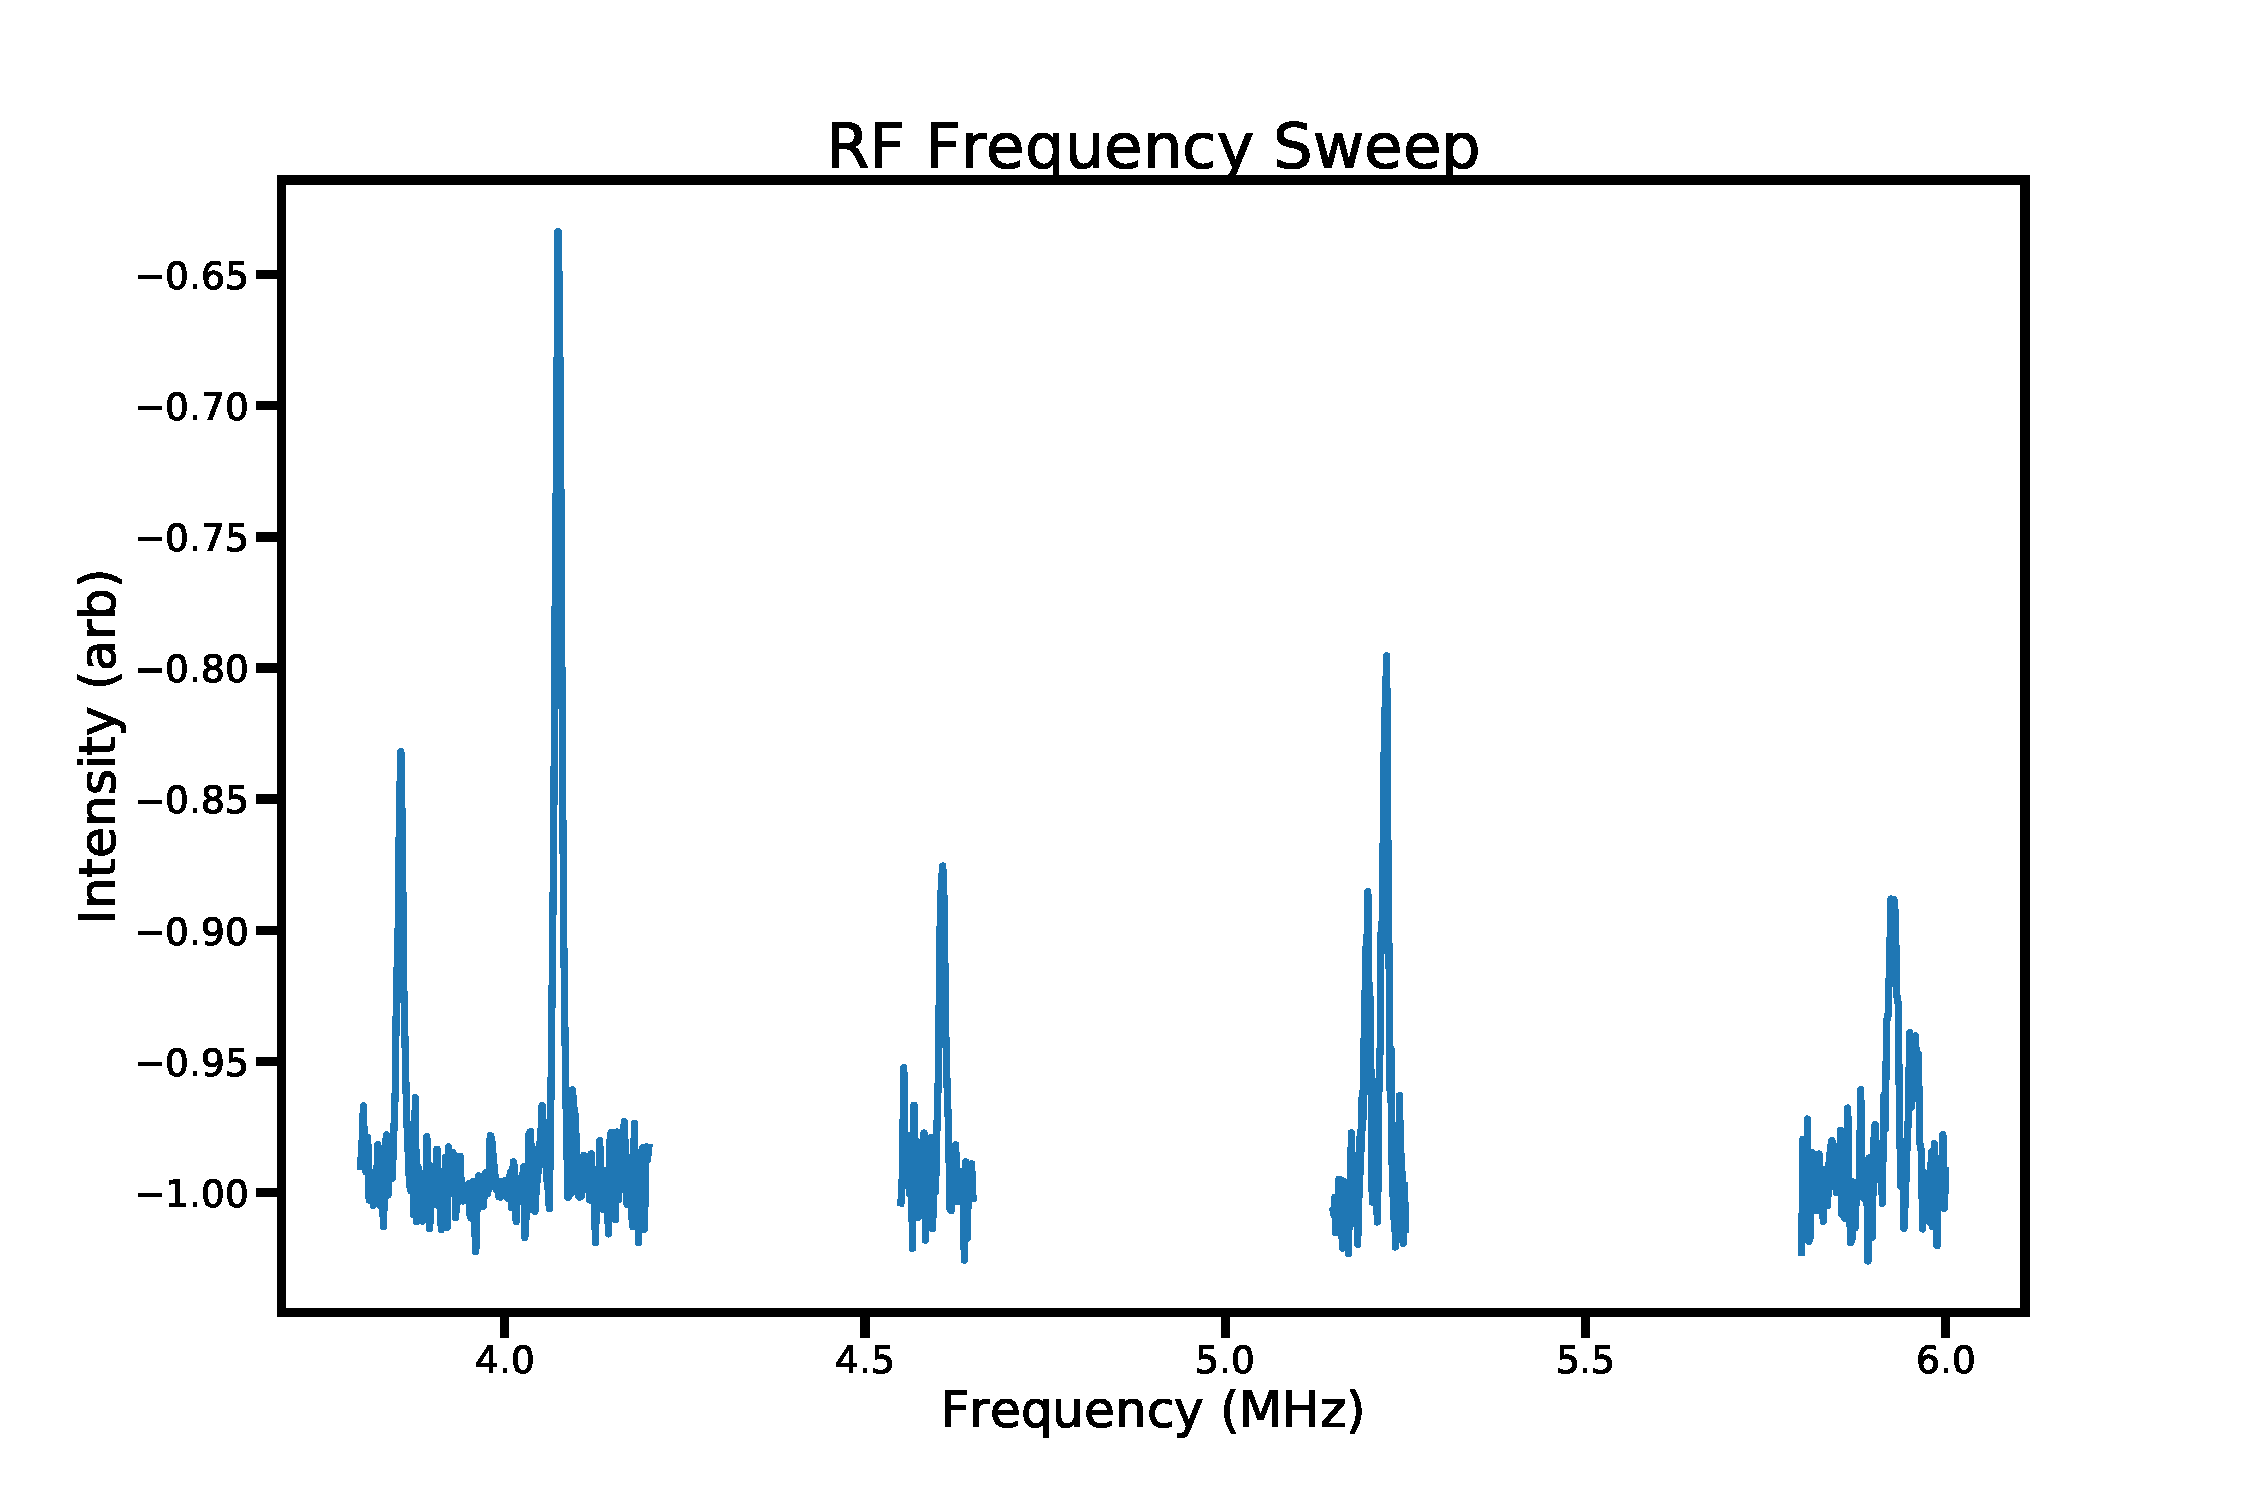
\includegraphics[width = 0.8\columnwidth]{Figures/FreqSweep.pdf} 
\caption[Frequency sweep of $^{29}$Si transitions]{Figure showing the peaks corresponding to the various $^{29}$Si nuclei coupled to the donor electron. The different transition frequencies correspond to different hyperfine couplings, based on the different distances from the $^{29}$Si to the donor impurity. The strength of the hyperfine coupling is determined by twice the difference between the transition frequency and the uncoupled transition of the $^{29}$Si nucleus of 2.91MHz \cite{Wolfowicz2016a}.}
\label{fig:si29freqsweep}
\end{figure}

Measurements of the Stark shift was undertaken at the maximum voltage before relaxation behaviour occurred of 15V (30V/mm), using the pulse sequence shown in figure \ref{fig:nuclearecho}.
Results are shown in figure \ref{fig:si29NoStark}.


\begin{figure}
\centering
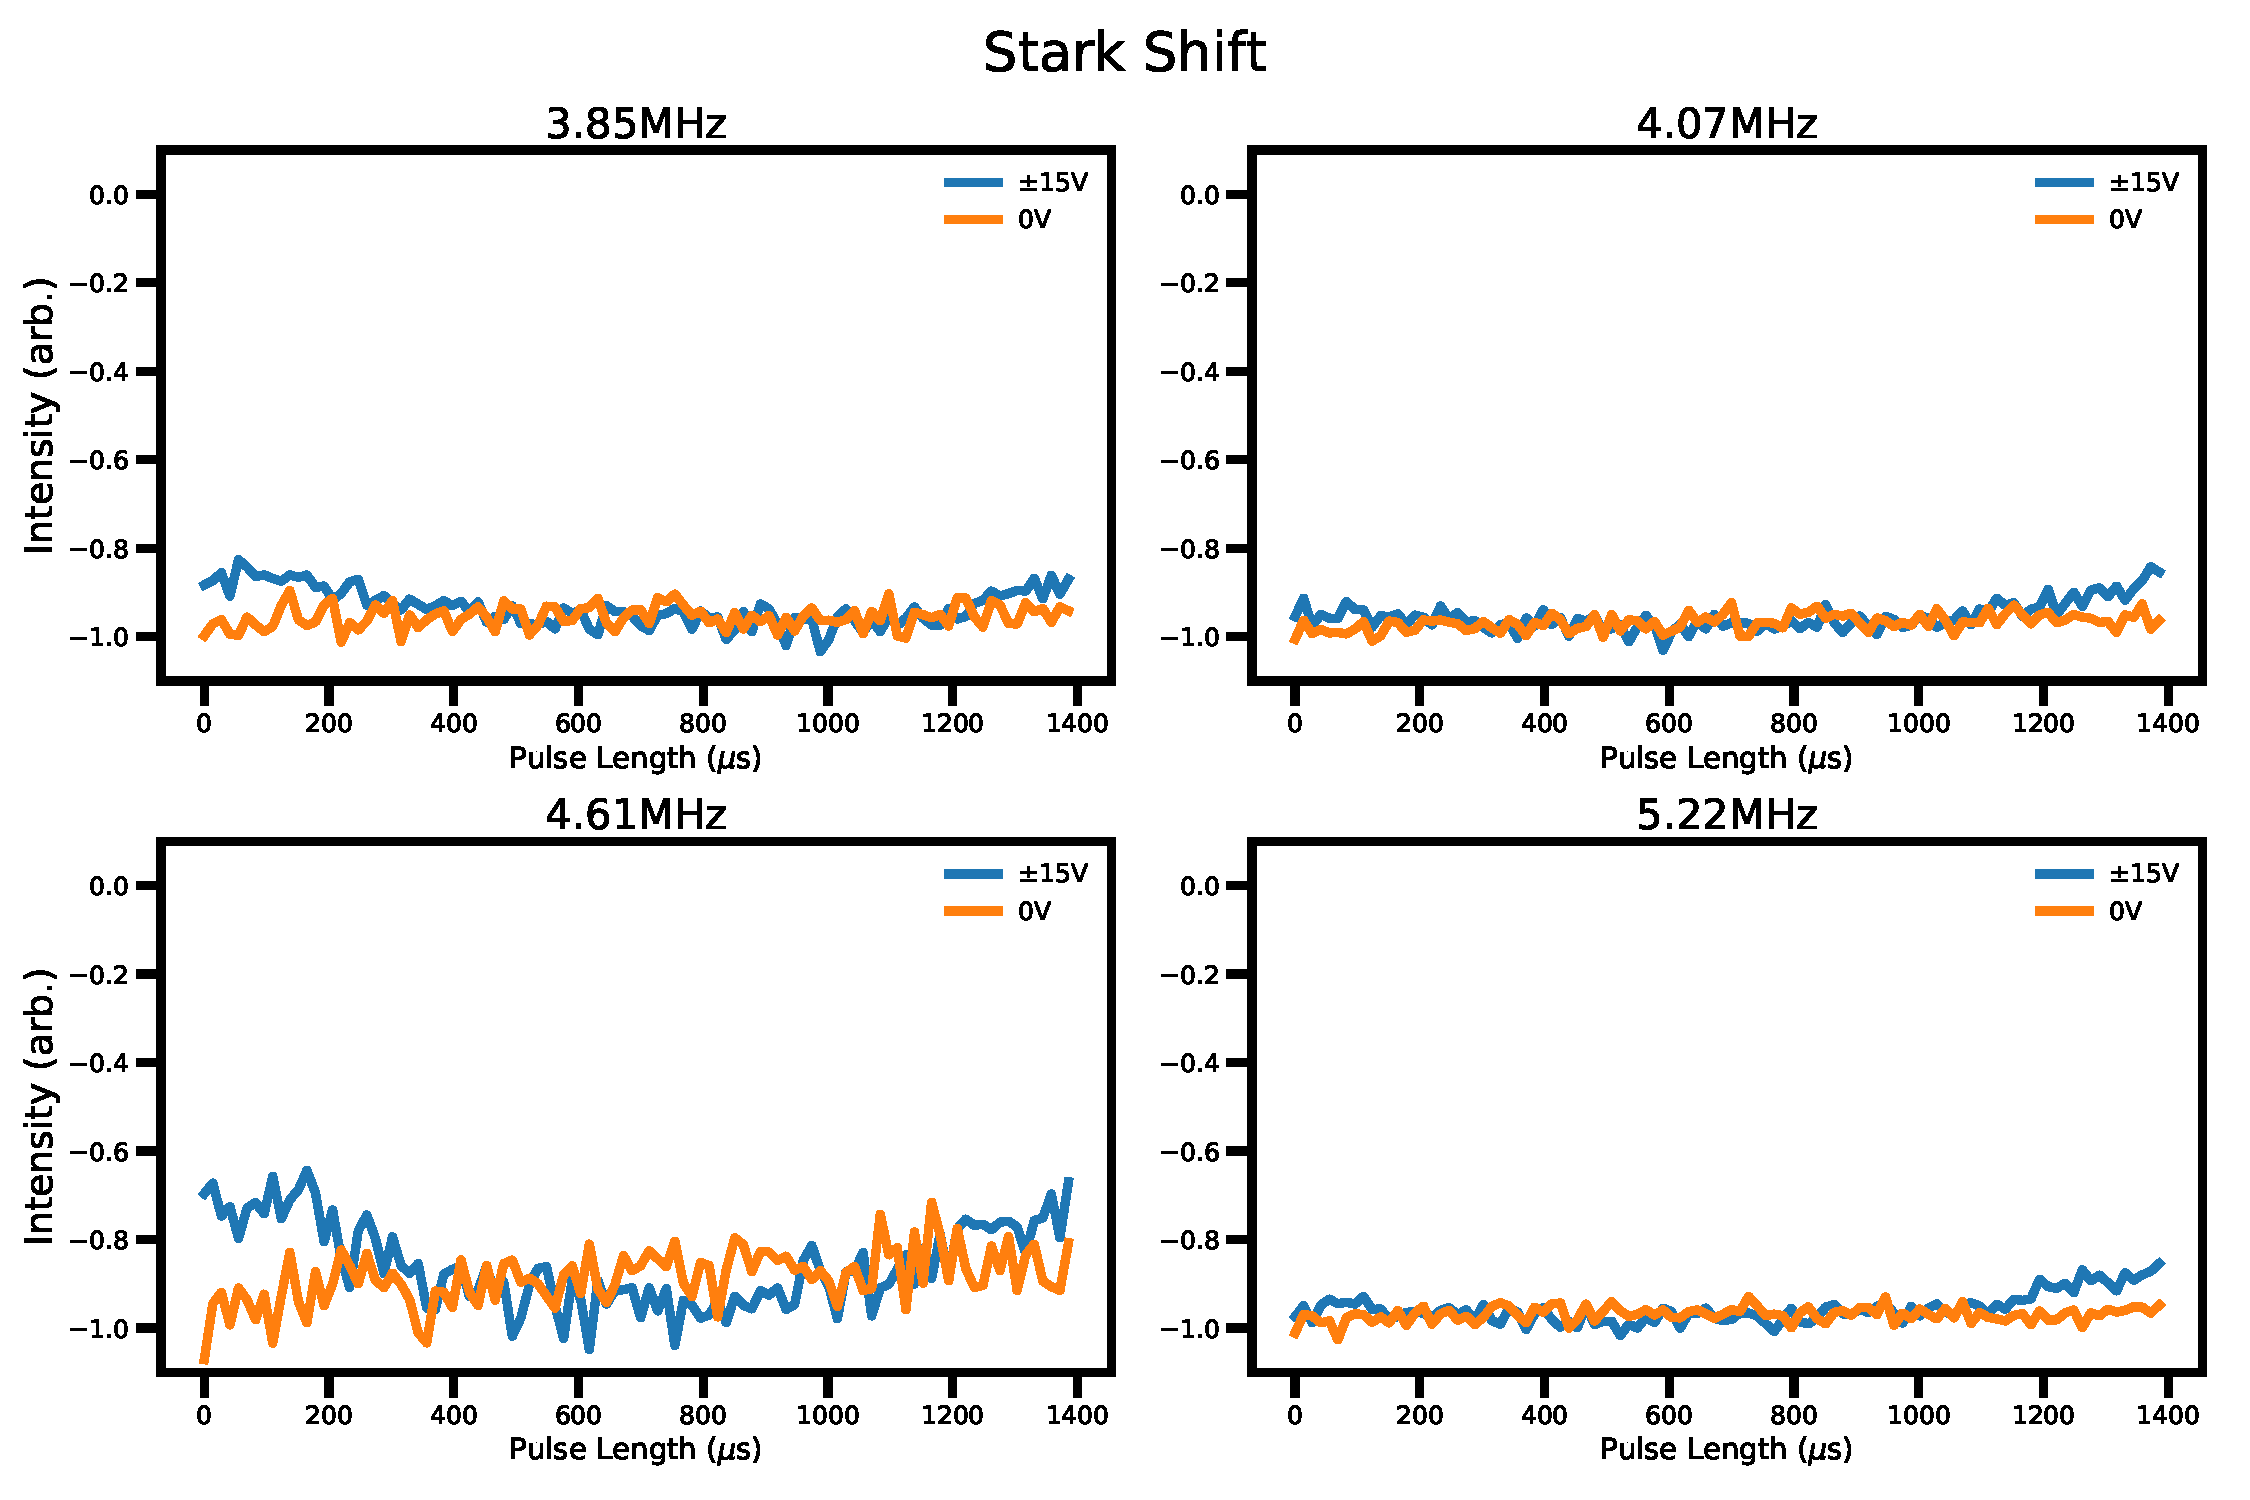
\includegraphics[width=\columnwidth]{Figures/StarkShiftMultiEchoReb.pdf}
\caption[Stark shift measurements of $^{29}$Si]{Figure shows the results of Stark shift experiments on 4 of the $^{29}$Si transitions, demonstrating that no obvious Stark shift is visible. Included is a 0 voltage sweep for comparison. The slight change in the signal when a voltage is applied is attributed to the beginning of relaxation behaviour being observed: as the $T_1$ of the electron is reduced a slight increase in signal is observed from spins previously saturated by repetition of the experiment returning to thermal equilibrium.} 
\label{fig:si29NoStark}
\end{figure}

These demonstrate that no Stark shift is observable at any of these transitions. 
The small change in the signal - getting slightly more negative relative to the 0 voltage case - is attributed to the slight reduction in $T_1$ of the electron increasing the signal by relaxing electrons previously saturated by the repetition rate of the experiment to thermal equilibrium. 
The change in signal cannot be attributed to the Stark shift as this would result in the signal becoming more positive initially, not more negative. 
Analysis of these results for upper bounding of the Stark shift parameter is made difficult by the unexpectedly strong Stark shift of the phosphorus nucleus.
At the voltage the experiment was conducted at the upper bound is quite large for each of the transitions, as seen in the table below.
For reference, the upper bound for the case that the voltage was equal to 140 V mm$^{-1}$ (as implied by the observed Stark shift of the phosphorus nucleus) is included. 

\begin{center}
\begin{tabular}{||c || c | c ||}
\hline
Transition (MHz)& $\eta_A$ 40V mm$^{-1}$ & $\eta_A$ 140V mm$^{-1}$\\
\hline
3.85 & 0.22 & 0.01\\
4.07 & 0.12 & 0.008\\
4.61 & 0.12 & 0.006\\
5.22 & 0.09 & 0.004\\
5.92 & 0.07 & 0.003\\
\hline
\end{tabular}
\end{center}

The resolution of the experiment is further limited by the pulse sequence used to measure the Stark shift, which renders the imaginary channel meaningless.
Repeating the experiment and using the full nuclear coherence transfer method would provide this imaginary channel.
This would improve the sensitivity of the experiment as the phase shift would then be proportional to the inverse sine of the frequency shift, which is a much larger and therefore more easily observable figure.
This experiment was implemented without difficulty on the phosphorus nucleus and a Stark shift in both channels observed.
However, despite multiple attempts it has yet to be performed successfully on the $^{29}$Si transitions.
This may be due to the reduced signal, due the significantly longer pulse sequence.
However this pulse sequence has been implemented successfully before on this system in \cite{Wolfowicz2016a}, suggesting that issues may be introduced by the presence of the copper plates.
These provide a much stronger thermal coupling to the environment, reducing the $T_1$ time from the expected many seconds to only 100~s of milliseconds. 
This may explain the fact that no signal can be observed when performing a full nuclear coherence transfer experiment on the $^{29}$Si transitions.
\\
% \inpu{}t{Text_Files/siP.tex}
% \input{Text_Files/epr.tex}

%%% APPENDICES AFTER THIS POINT
\clearpage
\appendix



% This ensures that the subsequent sections are being included as root
% items in the bookmark structure of your PDF reader.
\bookmarksetup{startatroot}
\backmatter

  % \begingroup
  %   \let\clearpage\relax
  %   \glsaddall
  %   \printglossary[type=\acronymtype]
  %   \newpage
  %   \printglossary
  % \endgroup
  \printindex
  \printbibliography
\end{document}
